\documentclass{article}\usepackage[]{graphicx}\usepackage[]{color}
% maxwidth is the original width if it is less than linewidth
% otherwise use linewidth (to make sure the graphics do not exceed the margin)
\makeatletter
\def\maxwidth{ %
  \ifdim\Gin@nat@width>\linewidth
    \linewidth
  \else
    \Gin@nat@width
  \fi
}
\makeatother

\definecolor{fgcolor}{rgb}{0.345, 0.345, 0.345}
\newcommand{\hlnum}[1]{\textcolor[rgb]{0.686,0.059,0.569}{#1}}%
\newcommand{\hlstr}[1]{\textcolor[rgb]{0.192,0.494,0.8}{#1}}%
\newcommand{\hlcom}[1]{\textcolor[rgb]{0.678,0.584,0.686}{\textit{#1}}}%
\newcommand{\hlopt}[1]{\textcolor[rgb]{0,0,0}{#1}}%
\newcommand{\hlstd}[1]{\textcolor[rgb]{0.345,0.345,0.345}{#1}}%
\newcommand{\hlkwa}[1]{\textcolor[rgb]{0.161,0.373,0.58}{\textbf{#1}}}%
\newcommand{\hlkwb}[1]{\textcolor[rgb]{0.69,0.353,0.396}{#1}}%
\newcommand{\hlkwc}[1]{\textcolor[rgb]{0.333,0.667,0.333}{#1}}%
\newcommand{\hlkwd}[1]{\textcolor[rgb]{0.737,0.353,0.396}{\textbf{#1}}}%
\let\hlipl\hlkwb

\usepackage{framed}
\makeatletter
\newenvironment{kframe}{%
 \def\at@end@of@kframe{}%
 \ifinner\ifhmode%
  \def\at@end@of@kframe{\end{minipage}}%
  \begin{minipage}{\columnwidth}%
 \fi\fi%
 \def\FrameCommand##1{\hskip\@totalleftmargin \hskip-\fboxsep
 \colorbox{shadecolor}{##1}\hskip-\fboxsep
     % There is no \\@totalrightmargin, so:
     \hskip-\linewidth \hskip-\@totalleftmargin \hskip\columnwidth}%
 \MakeFramed {\advance\hsize-\width
   \@totalleftmargin\z@ \linewidth\hsize
   \@setminipage}}%
 {\par\unskip\endMakeFramed%
 \at@end@of@kframe}
\makeatother

\definecolor{shadecolor}{rgb}{.97, .97, .97}
\definecolor{messagecolor}{rgb}{0, 0, 0}
\definecolor{warningcolor}{rgb}{1, 0, 1}
\definecolor{errorcolor}{rgb}{1, 0, 0}
\newenvironment{knitrout}{}{} % an empty environment to be redefined in TeX

\usepackage{alltt}
\usepackage[top=1in,bottom=1in,left=1in,right=1in]{geometry}

\usepackage{setspace}

\usepackage{hyperref}
\hypersetup{colorlinks=true, urlcolor=blue, breaklinks=true}

\newcommand{\link}[1]{\footnote{\color{blue}\href{#1}{#1}}}
\newcommand{\myhref}[1]{\href{#1}{#1}}

\usepackage{amsmath}
\usepackage{amssymb}
\usepackage{mathtools}
\usepackage{linguex}
\usepackage{natbib}

%\usepackage{Sweave}





\title{Plot and examine chains: Nat. stories}
\author{JD}
\IfFileExists{upquote.sty}{\usepackage{upquote}}{}
\begin{document}

\maketitle

\section{Preparations}

\begin{knitrout}
\definecolor{shadecolor}{rgb}{0.969, 0.969, 0.969}\color{fgcolor}\begin{kframe}
\begin{verbatim}
## 'data.frame':	32341 obs. of  5 variables:
##  $ pos      : Factor w/ 32341 levels "1.1.1","1.1.word",..: 2 1 578 579 577 919 920 918 1264 1265 ...
##  $ X1       : int  1 1 1 1 1 1 1 1 1 1 ...
##  $ word     : Factor w/ 3516 levels "-",",",":","!",..: 1575 1575 3506 3506 3506 3398 3398 3398 3172 3172 ...
##  $ freq     : num  1.23e+08 1.23e+08 5.78e+08 5.78e+08 5.78e+08 ...
##  $ otherfreq: logi  NA NA NA NA NA NA ...
##       pos       word item zone       freq
## 1   1.1.1         if    1    1  123141271
## 2   1.2.1        you    1    2  578117187
## 3   1.3.1       were    1    3  457504590
## 4   1.4.1         to    1    4 4223327232
## 5   1.5.1    journey    1    5    6826751
## 6   1.6.1         to    1    6 4223327232
## 7   1.7.1        the    1    7 9819942513
## 8   1.8.1      north    1    8   24140988
## 9   1.9.1         of    1    9 6162371881
## 10 1.10.1    england    1   10   21443938
## 11 1.11.1        you    1   11  578117187
## 12 1.12.1      would    1   12  319551796
## 13 1.13.1       come    1   13   69378970
## 14 1.14.1         to    1   14 4223327232
## 15 1.15.1          a    1   15 3213754375
## 16 1.16.1     valley    1   16    4303289
## 17 1.17.1       that    1   17 1746480437
## 18 1.18.1         is    1   18 1780724214
## 19 1.19.1 surrounded    1   19    4468786
## 20 1.20.1         by    1   20  877228367
## 'data.frame':	32333 obs. of  5 variables:
##  $ pos      : Factor w/ 32333 levels "1.1.1","1.1.word",..: 2 1 578 579 577 919 920 918 1264 1265 ...
##  $ X2       : int  2 2 2 2 2 2 2 2 2 2 ...
##  $ word     : Factor w/ 3511 levels "-",",",":","!",..: 1571 1571 3501 3501 3501 3393 3393 3393 3167 3167 ...
##  $ freq     : int  99632595 99632595 25245107 25245107 25245107 7751670 7751670 7751670 8148828 8148828 ...
##  $ otherfreq: num  2.67e+10 2.67e+10 1.23e+08 1.23e+08 1.23e+08 ...
## # A tibble: 10,256 x 5
## # Groups:   pos [10,256]
##    pos    word     item  zone    bigram
##    <chr>  <chr>   <int> <int>     <dbl>
##  1 1.1.1  if          1     1 0.00374  
##  2 1.2.1  you         1     2 0.205    
##  3 1.3.1  were        1     3 0.0134   
##  4 1.4.1  to          1     4 0.0178   
##  5 1.5.1  journey     1     5 0.0000148
##  6 1.6.1  to          1     6 0.122    
##  7 1.7.1  the         1     7 0.129    
##  8 1.8.1  north       1     8 0.000538 
##  9 1.9.1  of          1     9 0.0107   
## 10 1.10.1 england     1    10 0.000569 
## # ... with 10,246 more rows
## 'data.frame':	30823 obs. of  5 variables:
##  $ pos      : Factor w/ 30823 levels "1.10.1","1.10.2",..: 555 554 880 881 879 1213 1214 1212 1541 1542 ...
##  $ X3       : int  3 3 3 3 3 3 3 3 3 3 ...
##  $ word     : Factor w/ 3351 levels "-",",",":","!",..: 3342 3342 3238 3238 3238 3020 3020 3020 1588 1588 ...
##  $ freq     : int  19346858 19346858 553145 553145 553145 316331 316331 316331 492 492 ...
##  $ otherfreq: int  99632595 99632595 25245107 25245107 25245107 7751670 7751670 7751670 8148828 8148828 ...
## # A tibble: 9,760 x 5
## # Groups:   pos [9,760]
##    pos    word     item  zone   trigram
##    <chr>  <chr>   <int> <int>     <dbl>
##  1 1.2.1  you         1     2 0.194    
##  2 1.3.1  were        1     3 0.0219   
##  3 1.4.1  to          1     4 0.0408   
##  4 1.5.1  journey     1     5 0.0000604
##  5 1.6.1  to          1     6 0.279    
##  6 1.7.1  the         1     7 0.253    
##  7 1.8.1  north       1     8 0.000624 
##  8 1.9.1  of          1     9 0.0150   
##  9 1.10.1 england     1    10 0.141    
## 10 1.11.1 you         1    11 0.00171  
## # ... with 9,750 more rows
\end{verbatim}
\end{kframe}
\end{knitrout}


\section{Predictions}

Get chains and add information about words.

\begin{knitrout}
\definecolor{shadecolor}{rgb}{0.969, 0.969, 0.969}\color{fgcolor}\begin{kframe}
\begin{alltt}
\hlstd{burnin} \hlkwb{<-} \hlnum{400}

\hlstd{c1} \hlkwb{<-} \hlkwd{read.csv}\hlstd{(}\hlstr{"chains/natural_stories1/chain-0.csv"}\hlstd{)}

\hlstd{dataf} \hlkwb{<-} \hlkwd{select}\hlstd{(c1,} \hlkwd{starts_with}\hlstd{(}\hlstr{"predicted_mu_rt"}\hlstd{))}

\hlstd{dataf} \hlkwb{<-} \hlstd{dataf[burnin}\hlopt{:}\hlkwd{length}\hlstd{(dataf[,} \hlnum{1}\hlstd{]), ]}

\hlstd{c2} \hlkwb{<-} \hlkwd{read.csv}\hlstd{(}\hlstr{"chains/natural_stories2/chain-0.csv"}\hlstd{)}

\hlstd{dataf.c2} \hlkwb{<-} \hlkwd{select}\hlstd{(c2,} \hlkwd{starts_with}\hlstd{(}\hlstr{"predicted_mu_rt"}\hlstd{))}

\hlstd{dataf.c2} \hlkwb{<-} \hlstd{dataf.c2[burnin}\hlopt{:}\hlkwd{length}\hlstd{(dataf.c2[,} \hlnum{1}\hlstd{]), ]}

\hlstd{dataf} \hlkwb{<-} \hlkwd{rbind}\hlstd{(dataf, dataf.c2)}

\hlkwd{str}\hlstd{(dataf)}
\end{alltt}
\begin{verbatim}
## 'data.frame':	1614 obs. of  1312 variables:
##  $ predicted_mu_rt__0   : num  307 307 307 307 307 ...
##  $ predicted_mu_rt__1   : num  339 339 339 339 339 ...
##  $ predicted_mu_rt__2   : num  350 350 350 353 353 ...
##  $ predicted_mu_rt__3   : num  307 307 307 307 307 ...
##  $ predicted_mu_rt__4   : num  316 316 316 319 319 ...
##  $ predicted_mu_rt__5   : num  305 305 305 305 305 ...
##  $ predicted_mu_rt__6   : num  354 354 355 359 359 ...
##  $ predicted_mu_rt__7   : num  338 338 338 338 338 ...
##  $ predicted_mu_rt__8   : num  313 313 313 315 315 ...
##  $ predicted_mu_rt__9   : num  306 306 306 306 306 ...
##  $ predicted_mu_rt__10  : num  320 320 320 324 324 ...
##  $ predicted_mu_rt__11  : num  340 340 340 341 341 ...
##  $ predicted_mu_rt__12  : num  310 310 310 311 311 ...
##  $ predicted_mu_rt__13  : num  338 338 338 338 338 ...
##  $ predicted_mu_rt__14  : num  305 305 305 305 305 ...
##  $ predicted_mu_rt__15  : num  322 322 322 327 327 ...
##  $ predicted_mu_rt__16  : num  342 342 342 343 343 ...
##  $ predicted_mu_rt__17  : num  340 340 340 340 340 ...
##  $ predicted_mu_rt__18  : num  306 306 306 306 306 ...
##  $ predicted_mu_rt__19  : num  359 359 358 364 364 ...
##  $ predicted_mu_rt__20  : num  339 339 339 339 339 ...
##  $ predicted_mu_rt__21  : num  312 312 312 314 314 ...
##  $ predicted_mu_rt__22  : num  305 305 305 305 305 ...
##  $ predicted_mu_rt__23  : num  306 306 306 306 306 ...
##  $ predicted_mu_rt__24  : num  305 305 305 305 305 ...
##  $ predicted_mu_rt__25  : num  307 307 307 308 308 ...
##  $ predicted_mu_rt__26  : num  305 305 305 305 305 ...
##  $ predicted_mu_rt__27  : num  319 319 319 322 322 ...
##  $ predicted_mu_rt__28  : num  338 338 338 338 338 ...
##  $ predicted_mu_rt__29  : num  305 305 305 305 305 ...
##  $ predicted_mu_rt__30  : num  307 307 307 308 308 ...
##  $ predicted_mu_rt__31  : num  340 340 340 340 340 ...
##  $ predicted_mu_rt__32  : num  311 311 311 312 312 ...
##  $ predicted_mu_rt__33  : num  307 307 307 307 307 ...
##  $ predicted_mu_rt__34  : num  373 373 373 373 373 ...
##  $ predicted_mu_rt__35  : num  325 325 325 330 330 ...
##  $ predicted_mu_rt__36  : num  306 306 306 306 306 ...
##  $ predicted_mu_rt__37  : num  306 306 306 306 306 ...
##  $ predicted_mu_rt__38  : num  326 326 326 332 332 ...
##  $ predicted_mu_rt__39  : num  339 339 339 339 339 ...
##  $ predicted_mu_rt__40  : num  306 306 306 307 307 ...
##  $ predicted_mu_rt__41  : num  311 311 311 313 313 ...
##  $ predicted_mu_rt__42  : num  316 316 316 318 318 ...
##  $ predicted_mu_rt__43  : num  340 340 340 340 340 ...
##  $ predicted_mu_rt__44  : num  340 340 340 340 340 ...
##  $ predicted_mu_rt__45  : num  319 319 319 323 323 ...
##  $ predicted_mu_rt__46  : num  305 305 305 305 305 ...
##  $ predicted_mu_rt__47  : num  305 305 305 305 305 ...
##  $ predicted_mu_rt__48  : num  316 316 316 319 319 ...
##  $ predicted_mu_rt__49  : num  350 350 350 353 353 ...
##  $ predicted_mu_rt__50  : num  308 308 308 309 309 ...
##  $ predicted_mu_rt__51  : num  310 310 310 312 312 ...
##  $ predicted_mu_rt__52  : num  320 320 319 323 323 ...
##  $ predicted_mu_rt__53  : num  339 339 339 339 339 ...
##  $ predicted_mu_rt__54  : num  305 305 305 305 305 ...
##  $ predicted_mu_rt__55  : num  309 309 309 310 310 ...
##  $ predicted_mu_rt__56  : num  305 305 305 305 305 ...
##  $ predicted_mu_rt__57  : num  305 305 305 305 305 ...
##  $ predicted_mu_rt__58  : num  324 324 324 329 329 ...
##  $ predicted_mu_rt__59  : num  339 339 339 339 339 ...
##  $ predicted_mu_rt__60  : num  307 307 307 308 308 ...
##  $ predicted_mu_rt__61  : num  324 324 324 329 329 ...
##  $ predicted_mu_rt__62  : num  326 326 326 332 332 ...
##  $ predicted_mu_rt__63  : num  338 338 338 338 338 ...
##  $ predicted_mu_rt__64  : num  310 310 310 311 311 ...
##  $ predicted_mu_rt__65  : num  307 307 307 308 308 ...
##  $ predicted_mu_rt__66  : num  326 326 326 331 331 ...
##  $ predicted_mu_rt__67  : num  346 346 346 348 348 ...
##  $ predicted_mu_rt__68  : num  309 309 309 310 310 ...
##  $ predicted_mu_rt__69  : num  306 306 306 307 307 ...
##  $ predicted_mu_rt__70  : num  309 309 309 310 310 ...
##  $ predicted_mu_rt__71  : num  305 305 305 305 305 ...
##  $ predicted_mu_rt__72  : num  306 306 306 307 307 ...
##  $ predicted_mu_rt__73  : num  306 306 306 307 307 ...
##  $ predicted_mu_rt__74  : num  306 306 306 306 306 ...
##  $ predicted_mu_rt__75  : num  339 339 339 340 340 ...
##  $ predicted_mu_rt__76  : num  319 319 319 323 323 ...
##  $ predicted_mu_rt__77  : num  373 373 373 373 373 ...
##  $ predicted_mu_rt__78  : num  306 306 306 306 306 ...
##  $ predicted_mu_rt__79  : num  308 308 308 309 309 ...
##  $ predicted_mu_rt__80  : num  318 318 318 321 321 ...
##  $ predicted_mu_rt__81  : num  311 311 311 313 313 ...
##  $ predicted_mu_rt__82  : num  305 305 305 305 305 ...
##  $ predicted_mu_rt__83  : num  319 319 319 323 323 ...
##  $ predicted_mu_rt__84  : num  373 373 373 373 373 ...
##  $ predicted_mu_rt__85  : num  313 313 313 315 315 ...
##  $ predicted_mu_rt__86  : num  305 305 305 305 305 ...
##  $ predicted_mu_rt__87  : num  320 320 320 324 324 ...
##  $ predicted_mu_rt__88  : num  306 306 306 306 306 ...
##  $ predicted_mu_rt__89  : num  314 314 314 316 316 ...
##  $ predicted_mu_rt__90  : num  305 305 305 306 306 ...
##  $ predicted_mu_rt__91  : num  316 316 316 319 319 ...
##  $ predicted_mu_rt__92  : num  338 338 338 338 338 ...
##  $ predicted_mu_rt__93  : num  328 328 328 334 334 ...
##  $ predicted_mu_rt__94  : num  305 305 305 305 305 ...
##  $ predicted_mu_rt__95  : num  305 305 305 305 305 ...
##  $ predicted_mu_rt__96  : num  328 328 328 334 334 ...
##  $ predicted_mu_rt__97  : num  315 315 315 318 318 ...
##  $ predicted_mu_rt__98  : num  314 314 314 316 316 ...
##   [list output truncated]
\end{verbatim}
\begin{alltt}
\hlstd{ndraws} \hlkwb{<-} \hlkwd{length}\hlstd{(dataf[,} \hlnum{1}\hlstd{])}
\hlstd{nregions} \hlkwb{<-} \hlkwd{length}\hlstd{(dataf[}\hlnum{1}\hlstd{, ])}

\hlstd{ndraws}
\end{alltt}
\begin{verbatim}
## [1] 1614
\end{verbatim}
\begin{alltt}
\hlstd{nregions}
\end{alltt}
\begin{verbatim}
## [1] 1312
\end{verbatim}
\begin{alltt}
\hlstd{wordinfo} \hlkwb{<-} \hlkwd{read.csv}\hlstd{(}\hlstr{"additional_wordinfo.csv"}\hlstd{,} \hlkwc{sep} \hlstd{=} \hlstr{","}\hlstd{)}

\hlkwd{str}\hlstd{(wordinfo)}
\end{alltt}
\begin{verbatim}
## 'data.frame':	2091 obs. of  6 variables:
##  $ position   : int  1 2 3 4 5 6 7 8 9 10 ...
##  $ zone       : int  1 2 3 4 5 6 7 8 9 10 ...
##  $ item       : int  1 1 1 1 1 1 1 1 1 1 ...
##  $ sentence_no: int  1 1 1 1 1 1 1 1 1 1 ...
##  $ word       : Factor w/ 608 levels ",",":","'","''",..: 258 607 576 533 275 533 510 346 352 149 ...
##  $ record_RTs : Factor w/ 2 levels "no","yes": 2 2 2 2 2 2 2 2 2 2 ...
\end{verbatim}
\begin{alltt}
\hlstd{wordinfo} \hlkwb{<-} \hlkwd{left_join}\hlstd{(wordinfo, freqs,} \hlkwc{by} \hlstd{=} \hlkwd{c}\hlstd{(}\hlstr{"zone"}\hlstd{,} \hlstr{"item"}\hlstd{))}

\hlstd{wordinfo} \hlkwb{<-} \hlkwd{left_join}\hlstd{(wordinfo, freqs2,} \hlkwc{by} \hlstd{=} \hlkwd{c}\hlstd{(}\hlstr{"zone"}\hlstd{,} \hlstr{"item"}\hlstd{))}

\hlstd{wordinfo} \hlkwb{<-} \hlkwd{left_join}\hlstd{(wordinfo, freqs3,} \hlkwc{by} \hlstd{=} \hlkwd{c}\hlstd{(}\hlstr{"zone"}\hlstd{,} \hlstr{"item"}\hlstd{))}

\hlkwd{head}\hlstd{(wordinfo)}
\end{alltt}
\begin{verbatim}
##   position zone item sentence_no  word.x record_RTs pos.x  word.y
## 1        1    1    1           1      if        yes 1.1.1      if
## 2        2    2    1           1     you        yes 1.2.1     you
## 3        3    3    1           1    were        yes 1.3.1    were
## 4        4    4    1           1      to        yes 1.4.1      to
## 5        5    5    1           1 journey        yes 1.5.1 journey
## 6        6    6    1           1      to        yes 1.6.1      to
##         freq pos.y word.x.x       bigram   pos word.y.y      trigram
## 1  123141271 1.1.1       if 3.738225e-03  <NA>     <NA>           NA
## 2  578117187 1.2.1      you 2.050093e-01 1.2.1      you 1.941820e-01
## 3  457504590 1.3.1     were 1.340848e-02 1.3.1     were 2.191098e-02
## 4 4223327232 1.4.1       to 1.781147e-02 1.4.1       to 4.080811e-02
## 5    6826751 1.5.1  journey 1.477958e-05 1.5.1  journey 6.037678e-05
## 6 4223327232 1.6.1       to 1.215130e-01 1.6.1       to 2.793861e-01
\end{verbatim}
\begin{alltt}
\hlstd{real} \hlkwb{<-} \hlkwd{read.csv}\hlstd{(}\hlstr{"processed_wordinfo.tsv"}\hlstd{,} \hlkwc{sep} \hlstd{=} \hlstr{"\textbackslash{}t"}\hlstd{)}

\hlkwd{str}\hlstd{(real)}
\end{alltt}
\begin{verbatim}
## 'data.frame':	10256 obs. of  8 variables:
##  $ word       : Factor w/ 3104 levels "'Admiral","'admiral',",..: 1 2 3 4 5 6 7 8 9 10 ...
##  $ zone       : int  344 311 946 885 361 1040 716 390 842 606 ...
##  $ item       : int  9 9 6 8 9 6 1 4 2 8 ...
##  $ nItem      : int  76 78 82 70 75 79 85 88 92 73 ...
##  $ meanItemRT : num  426 420 324 352 406 ...
##  $ sdItemRT   : num  175 156 133 130 165 ...
##  $ gmeanItemRT: num  395 392 303 333 375 ...
##  $ gsdItemRT  : num  1.48 1.45 1.43 1.39 1.51 ...
\end{verbatim}
\begin{alltt}
\hlstd{real} \hlkwb{<-} \hlkwd{select}\hlstd{(real, word, zone, item, meanItemRT)}

\hlstd{test_wordinfo} \hlkwb{<-} \hlkwd{subset}\hlstd{(wordinfo, record_RTs} \hlopt{==} \hlstr{"yes"}\hlstd{)}  \hlcom{# keep only wordinfo for actual words}

\hlkwd{str}\hlstd{(test_wordinfo)}
\end{alltt}
\begin{verbatim}
## 'data.frame':	1931 obs. of  15 variables:
##  $ position   : int  1 2 3 4 5 6 7 8 9 10 ...
##  $ zone       : int  1 2 3 4 5 6 7 8 9 10 ...
##  $ item       : int  1 1 1 1 1 1 1 1 1 1 ...
##  $ sentence_no: int  1 1 1 1 1 1 1 1 1 1 ...
##  $ word.x     : Factor w/ 608 levels ",",":","'","''",..: 258 607 576 533 275 533 510 346 352 149 ...
##  $ record_RTs : Factor w/ 2 levels "no","yes": 2 2 2 2 2 2 2 2 2 2 ...
##  $ pos.x      : chr  "1.1.1" "1.2.1" "1.3.1" "1.4.1" ...
##  $ word.y     : chr  "if" "you" "were" "to" ...
##  $ freq       : num  1.23e+08 5.78e+08 4.58e+08 4.22e+09 6.83e+06 ...
##  $ pos.y      : chr  "1.1.1" "1.2.1" "1.3.1" "1.4.1" ...
##  $ word.x.x   : chr  "if" "you" "were" "to" ...
##  $ bigram     : num  3.74e-03 2.05e-01 1.34e-02 1.78e-02 1.48e-05 ...
##  $ pos        : chr  NA "1.2.1" "1.3.1" "1.4.1" ...
##  $ word.y.y   : chr  NA "you" "were" "to" ...
##  $ trigram    : num  NA 1.94e-01 2.19e-02 4.08e-02 6.04e-05 ...
\end{verbatim}
\begin{alltt}
\hlstd{test_wordinfo} \hlkwb{<-} \hlkwd{subset}\hlstd{(test_wordinfo, sentence_no} \hlopt \hlkwd{c}\hlstd{(}\hlnum{11}\hlopt{:}\hlnum{57}\hlstd{,} \hlnum{68}\hlopt{:}\hlnum{94}\hlstd{))}  \hlcom{# remove the first 10 sents in both stories}

\hlstd{test_wordinfo} \hlkwb{<-} \hlkwd{subset}\hlstd{(test_wordinfo, position} \hlopt{!=} \hlnum{1}\hlstd{)}  \hlcom{# remove first word}

\hlkwd{str}\hlstd{(test_wordinfo)}
\end{alltt}
\begin{verbatim}
## 'data.frame':	1312 obs. of  15 variables:
##  $ position   : int  2 3 4 5 6 7 8 9 10 11 ...
##  $ zone       : int  294 295 296 297 298 299 300 301 302 303 ...
##  $ item       : int  1 1 1 1 1 1 1 1 1 1 ...
##  $ sentence_no: int  11 11 11 11 11 11 11 11 11 11 ...
##  $ word.x     : Factor w/ 608 levels ",",":","'","''",..: 426 509 589 110 279 510 65 28 72 35 ...
##  $ record_RTs : Factor w/ 2 levels "no","yes": 2 2 2 2 2 2 2 2 2 2 ...
##  $ pos.x      : chr  "1.294.1" "1.295.1" "1.296.1" "1.297.1" ...
##  $ word.y     : chr  "said" "that" "whoever" "could" ...
##  $ freq       : num  1.72e+08 1.75e+09 1.32e+06 2.06e+08 7.60e+06 ...
##  $ pos.y      : chr  "1.294.1" "1.295.1" "1.296.1" "1.297.1" ...
##  $ word.x.x   : chr  "said" "that" "whoever" "could" ...
##  $ bigram     : num  1.84e-02 6.00e-02 8.99e-05 5.30e-03 7.02e-04 ...
##  $ pos        : chr  "1.294.1" "1.295.1" "1.296.1" "1.297.1" ...
##  $ word.y.y   : chr  "said" "that" "whoever" "could" ...
##  $ trigram    : num  0.018117 0.152912 0.000334 0.009856 0.003151 ...
\end{verbatim}
\begin{alltt}
\hlkwd{head}\hlstd{(test_wordinfo,} \hlkwc{n} \hlstd{=} \hlnum{50}\hlstd{)}
\end{alltt}
\begin{verbatim}
##     position zone item sentence_no       word.x record_RTs   pos.x
## 300        2  294    1          11         said        yes 1.294.1
## 301        3  295    1          11         that        yes 1.295.1
## 302        4  296    1          11      whoever        yes 1.296.1
## 303        5  297    1          11        could        yes 1.297.1
## 304        6  298    1          11         kill        yes 1.298.1
## 305        7  299    1          11          the        yes 1.299.1
## 306        8  300    1          11         boar        yes 1.300.1
## 307        9  301    1          11          and        yes 1.301.1
## 308       10  302    1          11        bring        yes 1.302.1
## 309       11  303    1          11           as        yes 1.303.1
## 310       12  304    1          11        proof        yes 1.304.1
## 311       13  305    1          11          its        yes 1.305.1
## 312       14  306    1          11         head        yes 1.306.1
## 313       15  307    1          11           to        yes 1.307.1
## 314       16  308    1          11          the        yes 1.308.1
## 315       17  309    1          11        manor        yes 1.309.1
## 316       18  310    1          11        house        yes 1.310.1
## 317       19  311    1          11        would        yes 1.311.1
## 318       20  312    1          11           be        yes 1.312.1
## 319       21  313    1          11     rewarded        yes 1.313.1
## 320       22  314    1          11         with        yes 1.314.1
## 321       23  315    1          11         land        yes 1.315.1
## 322       24  316    1          11          and        yes 1.316.1
## 324        2  319    1          12          was        yes 1.319.1
## 325        3  320    1          12          the        yes 1.320.1
## 326        4  321    1          12       people        yes 1.321.1
## 327        5  322    1          12           of        yes 1.322.1
## 328        6  323    1          12     bradford        yes 1.323.1
## 329        7  324    1          12          and        yes 1.324.1
## 330        8  325    1          12          the        yes 1.325.1
## 331        9  326    1          12       people        yes 1.326.1
## 332       10  327    1          12          who        yes 1.327.1
## 333       11  328    1          12         knew        yes 1.328.1
## 334       12  329    1          12         them        yes 1.329.1
## 335       13  330    1          12          who        yes 1.330.1
## 336       14  331    1          12     rejoiced        yes 1.331.1
## 337       15  332    1          12           at        yes 1.332.1
## 338       16  333    1          12         this        yes 1.333.1
## 339       17  334    1          12 proclamation        yes 1.334.1
## 340       18  335    1          12          but        yes 1.335.1
## 341       19  336    1          12          one        yes 1.336.1
## 342       20  337    1          12     question        yes 1.337.1
## 343       21  338    1          12     remained        yes 1.338.1
## 345       22  339    1          12          who        yes 1.339.1
## 346       23  340    1          12        would        yes 1.340.1
## 347       24  341    1          12         kill        yes 1.341.1
## 348       25  342    1          12          the        yes 1.342.1
## 350        2  345    1          13          the        yes 1.345.1
## 351        3  346    1          13     handsome        yes 1.346.1
## 352        4  347    1          13       reward        yes 1.347.1
##           word.y       freq   pos.y     word.x.x       bigram     pos
## 300         said  171981082 1.294.1         said 1.837667e-02 1.294.1
## 301         that 1746480437 1.295.1         that 5.996172e-02 1.295.1
## 302      whoever    1317362 1.296.1      whoever 8.987046e-05 1.296.1
## 303        could  205904563 1.297.1        could 5.299986e-03 1.297.1
## 304         kill    7599359 1.298.1         kill 7.024662e-04 1.298.1
## 305          the 9819942513 1.299.1          the 9.066528e-02 1.299.1
## 306         boar     309920 1.300.1         boar 5.952581e-06 1.300.1
## 307          and 4873010095 1.301.1          and 5.775039e-02 1.301.1
## 308        bring   21687869 1.302.1        bring 2.892165e-04 1.302.1
## 309           as 1139819594 1.303.1           as 8.973680e-04 1.303.1
## 310        proof    6786238 1.304.1        proof 2.416733e-04 1.304.1
## 311          its  259806050 1.305.1          its 4.627011e-05 1.305.1
## 312         head   48252042 1.306.1         head 2.875460e-03 1.306.1
## 313           to 4223327232 1.307.1           to 2.981735e-02 1.307.1
## 314          the 9819942513 1.308.1          the 1.291914e-01 1.308.1
## 315        manor     398133 1.309.1        manor 6.630792e-06 1.309.1
## 316        house   19438505 1.310.1        house 7.086828e-02 1.310.1
## 317        would  319551796 1.311.1        would 1.946858e-03 1.311.1
## 318           be  964072174 1.312.1           be 2.122336e-01 1.312.1
## 319     rewarded    1263320 1.313.1     rewarded 2.500746e-04 1.313.1
## 320         with 1110064802 1.314.1         with 1.857867e-01 1.314.1
## 321         land   36688838 1.315.1         land 1.073091e-04 1.315.1
## 322          and 4873010095 1.316.1          and 6.337243e-02 1.316.1
## 324          was 1140172617 1.319.1          was 1.989223e-01 1.319.1
## 325          the 9819942513 1.320.1          the 5.206902e-02 1.320.1
## 326       people  149869947 1.321.1       people 1.941252e-03 1.321.1
## 327           of 6162371881 1.322.1           of 3.854132e-02 1.322.1
## 328     bradford     737565 1.323.1     bradford 7.210048e-06 1.323.1
## 329          and 4873010095 1.324.1          and 4.146753e-02 1.324.1
## 330          the 9819942513 1.325.1          the 7.519450e-02 1.325.1
## 331       people  149869947 1.326.1       people 1.941252e-03 1.326.1
## 332          who  294018466 1.327.1          who 7.445483e-02 1.327.1
## 333         knew   37182349 1.328.1         knew 4.404730e-03 1.328.1
## 334         them  240201864 1.329.1         them 4.085030e-03 1.329.1
## 335          who  294018466 1.330.1          who 9.535147e-04 1.330.1
## 336     rejoiced     346775 1.331.1     rejoiced 2.729420e-05 1.331.1
## 337           at  654432238 1.332.1           at 1.192589e-01 1.332.1
## 338         this  599554050 1.333.1         this 1.710366e-02 1.333.1
## 339 proclamation     914548 1.334.1 proclamation 3.772137e-05 1.334.1
## 340          but  422070748 1.335.1          but 1.226836e-03 1.335.1
## 341          one  398913374 1.336.1          one 7.169409e-03 1.336.1
## 342     question   44123698 1.337.1     question 5.244597e-04 1.337.1
## 343     remained   15552573 1.338.1     remained 6.293670e-04 1.338.1
## 345          who  294018466 1.339.1          who 2.089226e-04 1.339.1
## 346        would  319551796 1.340.1        would 1.712385e-02 1.340.1
## 347         kill    7599359 1.341.1         kill 9.577070e-04 1.341.1
## 348          the 9819942513 1.342.1          the 9.066528e-02 1.342.1
## 350          the 9819942513 1.345.1          the 2.355679e-01 1.345.1
## 351     handsome    2651402 1.346.1     handsome 2.160766e-05 1.346.1
## 352       reward    3549720 1.347.1       reward 1.416609e-03 1.347.1
##         word.y.y      trigram
## 300         said 1.811739e-02
## 301         that 1.529123e-01
## 302      whoever 3.335828e-04
## 303        could 9.856203e-03
## 304         kill 3.150960e-03
## 305          the 6.740827e-02
## 306         boar 4.020331e-04
## 307          and 4.754166e-02
## 308        bring 0.000000e+00
## 309           as 6.073700e-04
## 310        proof 2.569109e-03
## 311          its 7.260477e-05
## 312         head 0.000000e+00
## 313           to 3.210978e-02
## 314          the 1.840135e-01
## 315        manor 1.295780e-05
## 316        house 1.561876e-01
## 317        would 8.860535e-04
## 318           be 2.020664e-01
## 319     rewarded 3.741690e-04
## 320         with 2.214277e-01
## 321         land 4.230789e-03
## 322          and 9.392210e-02
## 324          was 2.133987e-01
## 325          the 6.906550e-02
## 326       people 3.502748e-04
## 327           of 1.445975e-01
## 328     bradford 1.990933e-05
## 329          and 5.203574e-02
## 330          the 5.832925e-02
## 331       people 2.516839e-03
## 332          who 9.393871e-02
## 333         knew 6.665208e-03
## 334         them 1.454282e-02
## 335          who 1.185060e-04
## 336     rejoiced 0.000000e+00
## 337           at 1.264798e-01
## 338         this 6.506916e-02
## 339 proclamation 1.170355e-05
## 340          but 6.190308e-04
## 341          one 0.000000e+00
## 342     question 1.136154e-03
## 343     remained 5.286453e-03
## 345          who 8.819624e-03
## 346        would 3.807237e-02
## 347         kill 2.164764e-03
## 348          the 8.011123e-02
## 350          the 2.435807e-01
## 351     handsome 0.000000e+00
## 352       reward 6.550856e-04
\end{verbatim}
\begin{alltt}
\hlstd{combined} \hlkwb{<-} \hlkwd{left_join}\hlstd{(test_wordinfo, real,} \hlkwc{by} \hlstd{=} \hlkwd{c}\hlstd{(}\hlstr{"item"}\hlstd{,} \hlstr{"zone"}\hlstd{))}

\hlkwd{str}\hlstd{(combined)}
\end{alltt}
\begin{verbatim}
## 'data.frame':	1312 obs. of  17 variables:
##  $ position   : int  2 3 4 5 6 7 8 9 10 11 ...
##  $ zone       : int  294 295 296 297 298 299 300 301 302 303 ...
##  $ item       : int  1 1 1 1 1 1 1 1 1 1 ...
##  $ sentence_no: int  11 11 11 11 11 11 11 11 11 11 ...
##  $ word.x     : Factor w/ 608 levels ",",":","'","''",..: 426 509 589 110 279 510 65 28 72 35 ...
##  $ record_RTs : Factor w/ 2 levels "no","yes": 2 2 2 2 2 2 2 2 2 2 ...
##  $ pos.x      : chr  "1.294.1" "1.295.1" "1.296.1" "1.297.1" ...
##  $ word.y     : chr  "said" "that" "whoever" "could" ...
##  $ freq       : num  1.72e+08 1.75e+09 1.32e+06 2.06e+08 7.60e+06 ...
##  $ pos.y      : chr  "1.294.1" "1.295.1" "1.296.1" "1.297.1" ...
##  $ word.x.x   : chr  "said" "that" "whoever" "could" ...
##  $ bigram     : num  1.84e-02 6.00e-02 8.99e-05 5.30e-03 7.02e-04 ...
##  $ pos        : chr  "1.294.1" "1.295.1" "1.296.1" "1.297.1" ...
##  $ word.y.y   : chr  "said" "that" "whoever" "could" ...
##  $ trigram    : num  0.018117 0.152912 0.000334 0.009856 0.003151 ...
##  $ word       : Factor w/ 3104 levels "'Admiral","'admiral',",..: 2297 2712 3024 628 1485 2717 351 164 402 224 ...
##  $ meanItemRT : num  313 307 338 308 311 ...
\end{verbatim}
\begin{alltt}
\hlcom{# Test that we match words between wordinfo and freq dataframes: We should}
\hlcom{# only see rows in which non-alphanumeric characters appear on word.x (-,')}
\hlkwd{subset}\hlstd{(combined, word.x} \hlopt{!=} \hlstd{word.y)}
\end{alltt}
\begin{verbatim}
##      position zone item sentence_no        word.x record_RTs   pos.x
## 203        23  516    1          21  quick-witted        yes 1.516.1
## 210        30  523    1          21          what        yes 1.523.1
## 425        15  764    1          34          what        yes 1.764.1
## 449         8  800    1          40             i        yes 1.800.1
## 1048        5  707    2          85 hide-and-seek        yes 2.707.1
## 1088        5  749    2          86        peeked        yes 2.749.1
##      word.y      freq   pos.y word.x.x       bigram     pos word.y.y
## 203   quick   7462194 1.516.1    quick 9.307526e-05 1.516.1    quick
## 210       ' 836175651 1.523.1        ' 5.311628e-03 1.523.1        '
## 425       ' 836175651 1.764.1        ' 5.311628e-03 1.764.1        '
## 449       ' 836175651 1.800.1        ' 5.311628e-03 1.800.1        '
## 1048   hide   4034362 2.707.1     hide 4.999843e-04 2.707.1     hide
## 1088 peaked    445987 2.749.1   peaked 0.000000e+00 2.749.1   peaked
##           trigram          word meanItemRT
## 203  0.0011560455  quick-witted   372.9167
## 210  0.0092635573         'What   327.2588
## 425  0.0697574637         'What   335.6429
## 449  0.0849277633            'I   315.3333
## 1048 0.0009258993 hide-and-seek   363.7500
## 1088 0.0000000000        peaked   359.3556
\end{verbatim}
\begin{alltt}
\hlkwd{subset}\hlstd{(combined, word.x} \hlopt{!=} \hlstd{word.x.x)}
\end{alltt}
\begin{verbatim}
##      position zone item sentence_no        word.x record_RTs   pos.x
## 203        23  516    1          21  quick-witted        yes 1.516.1
## 210        30  523    1          21          what        yes 1.523.1
## 425        15  764    1          34          what        yes 1.764.1
## 449         8  800    1          40             i        yes 1.800.1
## 1048        5  707    2          85 hide-and-seek        yes 2.707.1
## 1088        5  749    2          86        peeked        yes 2.749.1
##      word.y      freq   pos.y word.x.x       bigram     pos word.y.y
## 203   quick   7462194 1.516.1    quick 9.307526e-05 1.516.1    quick
## 210       ' 836175651 1.523.1        ' 5.311628e-03 1.523.1        '
## 425       ' 836175651 1.764.1        ' 5.311628e-03 1.764.1        '
## 449       ' 836175651 1.800.1        ' 5.311628e-03 1.800.1        '
## 1048   hide   4034362 2.707.1     hide 4.999843e-04 2.707.1     hide
## 1088 peaked    445987 2.749.1   peaked 0.000000e+00 2.749.1   peaked
##           trigram          word meanItemRT
## 203  0.0011560455  quick-witted   372.9167
## 210  0.0092635573         'What   327.2588
## 425  0.0697574637         'What   335.6429
## 449  0.0849277633            'I   315.3333
## 1048 0.0009258993 hide-and-seek   363.7500
## 1088 0.0000000000        peaked   359.3556
\end{verbatim}
\begin{alltt}
\hlkwd{subset}\hlstd{(combined, word.x} \hlopt{!=} \hlstd{word.y.y)}
\end{alltt}
\begin{verbatim}
##      position zone item sentence_no        word.x record_RTs   pos.x
## 203        23  516    1          21  quick-witted        yes 1.516.1
## 210        30  523    1          21          what        yes 1.523.1
## 425        15  764    1          34          what        yes 1.764.1
## 449         8  800    1          40             i        yes 1.800.1
## 1048        5  707    2          85 hide-and-seek        yes 2.707.1
## 1088        5  749    2          86        peeked        yes 2.749.1
##      word.y      freq   pos.y word.x.x       bigram     pos word.y.y
## 203   quick   7462194 1.516.1    quick 9.307526e-05 1.516.1    quick
## 210       ' 836175651 1.523.1        ' 5.311628e-03 1.523.1        '
## 425       ' 836175651 1.764.1        ' 5.311628e-03 1.764.1        '
## 449       ' 836175651 1.800.1        ' 5.311628e-03 1.800.1        '
## 1048   hide   4034362 2.707.1     hide 4.999843e-04 2.707.1     hide
## 1088 peaked    445987 2.749.1   peaked 0.000000e+00 2.749.1   peaked
##           trigram          word meanItemRT
## 203  0.0011560455  quick-witted   372.9167
## 210  0.0092635573         'What   327.2588
## 425  0.0697574637         'What   335.6429
## 449  0.0849277633            'I   315.3333
## 1048 0.0009258993 hide-and-seek   363.7500
## 1088 0.0000000000        peaked   359.3556
\end{verbatim}
\begin{alltt}
\hlkwd{head}\hlstd{(combined)}
\end{alltt}
\begin{verbatim}
##   position zone item sentence_no  word.x record_RTs   pos.x  word.y
## 1        2  294    1          11    said        yes 1.294.1    said
## 2        3  295    1          11    that        yes 1.295.1    that
## 3        4  296    1          11 whoever        yes 1.296.1 whoever
## 4        5  297    1          11   could        yes 1.297.1   could
## 5        6  298    1          11    kill        yes 1.298.1    kill
## 6        7  299    1          11     the        yes 1.299.1     the
##         freq   pos.y word.x.x       bigram     pos word.y.y      trigram
## 1  171981082 1.294.1     said 1.837667e-02 1.294.1     said 0.0181173936
## 2 1746480437 1.295.1     that 5.996172e-02 1.295.1     that 0.1529123104
## 3    1317362 1.296.1  whoever 8.987046e-05 1.296.1  whoever 0.0003335828
## 4  205904563 1.297.1    could 5.299986e-03 1.297.1    could 0.0098562027
## 5    7599359 1.298.1     kill 7.024662e-04 1.298.1     kill 0.0031509596
## 6 9819942513 1.299.1      the 9.066528e-02 1.299.1      the 0.0674082729
##      word meanItemRT
## 1    said   313.4706
## 2    that   306.6118
## 3 whoever   338.4706
## 4   could   308.4535
## 5    kill   310.8372
## 6     the   297.8235
\end{verbatim}
\begin{alltt}
\hlkwd{tail}\hlstd{(combined)}
\end{alltt}
\begin{verbatim}
##      position zone item sentence_no    word.x record_RTs   pos.x
## 1307       45  984    2          94     about        yes 2.984.1
## 1308       46  985    2          94     their        yes 2.985.1
## 1309       47  986    2          94 wonderful        yes 2.986.1
## 1310       48  987    2          94   journey        yes 2.987.1
## 1311       49  988    2          94    around        yes 2.988.1
## 1312       50  989    2          94       the        yes 2.989.1
##         word.y       freq   pos.y  word.x.x       bigram     pos
## 1307     about  265782619 2.984.1     about 3.944663e-04 2.984.1
## 1308     their  438887121 2.985.1     their 1.587209e-02 2.985.1
## 1309 wonderful    6181671 2.986.1 wonderful 6.579596e-05 2.986.1
## 1310   journey    6826751 2.987.1   journey 7.433265e-04 2.987.1
## 1311    around   66671286 2.988.1    around 2.186399e-03 2.988.1
## 1312       the 9819942513 2.989.1       the 2.829297e-01 2.989.1
##       word.y.y      trigram      word meanItemRT
## 1307     about 0.0041000859     about   314.8387
## 1308     their 0.0962324267     their   306.1720
## 1309 wonderful 0.0001680682 wonderful   320.0426
## 1310   journey 0.0011427780   journey   320.3441
## 1311    around 0.0000000000    around   375.0426
## 1312       the 0.7358970923       the   433.3913
\end{verbatim}
\end{kframe}
\end{knitrout}

Store the result into one dataframe.

\begin{knitrout}
\definecolor{shadecolor}{rgb}{0.969, 0.969, 0.969}\color{fgcolor}\begin{kframe}
\begin{alltt}
\hlstd{data.all} \hlkwb{<-} \hlkwd{data.frame}\hlstd{(}\hlkwc{Region} \hlstd{=} \hlkwd{rep}\hlstd{(}\hlkwd{paste}\hlstd{(}\hlstr{"No_"}\hlstd{,} \hlkwd{str_pad}\hlstd{(}\hlnum{1}\hlopt{:}\hlstd{(nregions),} \hlkwc{width} \hlstd{=} \hlnum{4}\hlstd{,}
    \hlkwc{pad} \hlstd{=} \hlstr{"0"}\hlstd{),} \hlkwc{sep} \hlstd{=} \hlstr{""}\hlstd{),} \hlkwc{each} \hlstd{= ndraws),} \hlkwc{RT} \hlstd{=} \hlkwd{c}\hlstd{(dataf[}\hlnum{1}\hlopt{:}\hlstd{ndraws, ],} \hlkwc{recursive} \hlstd{=} \hlnum{TRUE}\hlstd{,}
    \hlkwc{use.names} \hlstd{=} \hlnum{FALSE}\hlstd{),} \hlkwc{Observed} \hlstd{=} \hlkwd{rep}\hlstd{(combined}\hlopt{$}\hlstd{meanItemRT[}\hlnum{1}\hlopt{:}\hlstd{(nregions)],} \hlkwc{each} \hlstd{= ndraws),}
    \hlkwc{Word} \hlstd{=} \hlkwd{rep}\hlstd{(combined}\hlopt{$}\hlstd{word.y[}\hlnum{1}\hlopt{:}\hlstd{(nregions)],} \hlkwc{each} \hlstd{= ndraws),} \hlkwc{Item} \hlstd{=} \hlkwd{rep}\hlstd{(combined}\hlopt{$}\hlstd{item[}\hlnum{1}\hlopt{:}\hlstd{(nregions)],}
        \hlkwc{each} \hlstd{= ndraws),} \hlkwc{Sentence_no} \hlstd{=} \hlkwd{rep}\hlstd{(}\hlkwd{as.numeric}\hlstd{(}\hlkwd{as.factor}\hlstd{(combined}\hlopt{$}\hlstd{sentence_no)),}
        \hlkwc{each} \hlstd{= ndraws),} \hlkwc{Position} \hlstd{=} \hlkwd{rep}\hlstd{(combined}\hlopt{$}\hlstd{position[}\hlnum{1}\hlopt{:}\hlstd{(nregions)],} \hlkwc{each} \hlstd{= ndraws),}
    \hlkwc{Freq} \hlstd{=} \hlkwd{rep}\hlstd{(combined}\hlopt{$}\hlstd{freq[}\hlnum{1}\hlopt{:}\hlstd{(nregions)],} \hlkwc{each} \hlstd{= ndraws),} \hlkwc{Bigram} \hlstd{=} \hlkwd{rep}\hlstd{(combined}\hlopt{$}\hlstd{bigram[}\hlnum{1}\hlopt{:}\hlstd{(nregions)],}
        \hlkwc{each} \hlstd{= ndraws),} \hlkwc{Trigram} \hlstd{=} \hlkwd{rep}\hlstd{(combined}\hlopt{$}\hlstd{trigram[}\hlnum{1}\hlopt{:}\hlstd{(nregions)],} \hlkwc{each} \hlstd{= ndraws))}

\hlcom{# we remove one outlier word (Bradford) (614 ms, while mean of all other}
\hlcom{# words below 500 ms)}
\hlstd{data.all} \hlkwb{<-} \hlkwd{subset}\hlstd{(data.all, Observed} \hlopt{<} \hlnum{500}\hlstd{)}

\hlkwd{str}\hlstd{(data.all)}
\end{alltt}
\begin{verbatim}
## 'data.frame':	2115954 obs. of  10 variables:
##  $ Region     : Factor w/ 1312 levels "No_0001","No_0002",..: 1 1 1 1 1 1 1 1 1 1 ...
##  $ RT         : num  307 307 307 307 307 ...
##  $ Observed   : num  313 313 313 313 313 ...
##  $ Word       : Factor w/ 471 levels "'","a","able",..: 330 330 330 330 330 330 330 330 330 330 ...
##  $ Item       : int  1 1 1 1 1 1 1 1 1 1 ...
##  $ Sentence_no: num  1 1 1 1 1 1 1 1 1 1 ...
##  $ Position   : int  2 2 2 2 2 2 2 2 2 2 ...
##  $ Freq       : num  1.72e+08 1.72e+08 1.72e+08 1.72e+08 1.72e+08 ...
##  $ Bigram     : num  0.0184 0.0184 0.0184 0.0184 0.0184 ...
##  $ Trigram    : num  0.0181 0.0181 0.0181 0.0181 0.0181 ...
\end{verbatim}
\begin{alltt}
\hlkwd{head}\hlstd{(data.all)}
\end{alltt}
\begin{verbatim}
##    Region    RT Observed Word Item Sentence_no Position      Freq
## 1 No_0001 306.6 313.4706 said    1           1        2 171981082
## 2 No_0001 306.6 313.4706 said    1           1        2 171981082
## 3 No_0001 306.7 313.4706 said    1           1        2 171981082
## 4 No_0001 307.1 313.4706 said    1           1        2 171981082
## 5 No_0001 307.1 313.4706 said    1           1        2 171981082
## 6 No_0001 307.1 313.4706 said    1           1        2 171981082
##       Bigram    Trigram
## 1 0.01837667 0.01811739
## 2 0.01837667 0.01811739
## 3 0.01837667 0.01811739
## 4 0.01837667 0.01811739
## 5 0.01837667 0.01811739
## 6 0.01837667 0.01811739
\end{verbatim}
\begin{alltt}
\hlkwd{tail}\hlstd{(data.all)}
\end{alltt}
\begin{verbatim}
##          Region    RT Observed Word Item Sentence_no Position       Freq
## 2117563 No_1312 305.2 433.3913  the    2          70       50 9819942513
## 2117564 No_1312 305.2 433.3913  the    2          70       50 9819942513
## 2117565 No_1312 305.2 433.3913  the    2          70       50 9819942513
## 2117566 No_1312 305.2 433.3913  the    2          70       50 9819942513
## 2117567 No_1312 305.2 433.3913  the    2          70       50 9819942513
## 2117568 No_1312 305.2 433.3913  the    2          70       50 9819942513
##            Bigram   Trigram
## 2117563 0.2829297 0.7358971
## 2117564 0.2829297 0.7358971
## 2117565 0.2829297 0.7358971
## 2117566 0.2829297 0.7358971
## 2117567 0.2829297 0.7358971
## 2117568 0.2829297 0.7358971
\end{verbatim}
\begin{alltt}
\hlkwd{subset}\hlstd{(data.all, Region} \hlopt{==} \hlstr{"No_1311"}\hlstd{)}\hlopt{$}\hlstd{Word[}\hlnum{1}\hlstd{]}  \hlcom{#should be word around}
\end{alltt}
\begin{verbatim}
## [1] around
## 471 Levels: ' a able about across advance after ago all almost ... you
\end{verbatim}
\begin{alltt}
\hlkwd{subset}\hlstd{(data.all, Region} \hlopt{==} \hlstr{"No_1311"}\hlstd{)}\hlopt{$}\hlstd{Word[ndraws]}  \hlcom{#should be word around}
\end{alltt}
\begin{verbatim}
## [1] around
## 471 Levels: ' a able about across advance after ago all almost ... you
\end{verbatim}
\begin{alltt}
\hlkwd{length}\hlstd{(}\hlkwd{subset}\hlstd{(data.all, Region} \hlopt{==} \hlstr{"No_1311"}\hlstd{)}\hlopt{$}\hlstd{Word)}  \hlcom{#should be ndraws == 1614}
\end{alltt}
\begin{verbatim}
## [1] 1614
\end{verbatim}
\end{kframe}
\end{knitrout}

We check that all predicted RTs within a sensible range (higher than 100 ms and below 1,000 ms:

\begin{knitrout}
\definecolor{shadecolor}{rgb}{0.969, 0.969, 0.969}\color{fgcolor}\begin{kframe}
\begin{alltt}
\hlkwd{subset}\hlstd{(data.all, RT} \hlopt{<} \hlnum{100} \hlopt{|} \hlstd{RT} \hlopt{>} \hlnum{1000}\hlstd{)}
\end{alltt}
\begin{verbatim}
##  [1] Region      RT          Observed    Word        Item       
##  [6] Sentence_no Position    Freq        Bigram      Trigram    
## <0 rows> (or 0-length row.names)
\end{verbatim}
\end{kframe}
\end{knitrout}

Summarise data for modeling. Below are explored models.

\begin{knitrout}
\definecolor{shadecolor}{rgb}{0.969, 0.969, 0.969}\color{fgcolor}\begin{kframe}
\begin{alltt}
\hlstd{data.model} \hlkwb{<-} \hlstd{data.all} \hlopt \hlkwd{group_by}\hlstd{(Item, Region)} \hlopt \hlkwd{summarise}\hlstd{(}\hlkwc{RT} \hlstd{=} \hlkwd{mean}\hlstd{(RT),}
    \hlkwc{Position} \hlstd{=} \hlkwd{first}\hlstd{(Position),} \hlkwc{Freq} \hlstd{=} \hlkwd{first}\hlstd{(Freq),} \hlkwc{Bigram} \hlstd{=} \hlkwd{first}\hlstd{(Bigram),}
    \hlkwc{Trigram} \hlstd{=} \hlkwd{first}\hlstd{(Trigram),} \hlkwc{Observed} \hlstd{=} \hlkwd{first}\hlstd{(Observed),} \hlkwc{Sentence_no} \hlstd{=} \hlkwd{first}\hlstd{(Sentence_no),}
    \hlkwc{Word} \hlstd{=} \hlkwd{first}\hlstd{(}\hlkwd{as.character}\hlstd{(Word)))}
\end{alltt}


{\ttfamily\noindent\itshape\color{messagecolor}{\#\# `summarise()` has grouped output by 'Item'. You can override using the `.groups` argument.}}\begin{alltt}
\hlstd{data.model} \hlkwb{<-} \hlstd{data.model} \hlopt \hlkwd{ungroup}\hlstd{()}

\hlstd{data.model}\hlopt{$}\hlstd{Nchar} \hlkwb{<-} \hlkwd{nchar}\hlstd{(data.model}\hlopt{$}\hlstd{Word)}

\hlcom{# for each story, we calculate the absolute position of a word in that}
\hlcom{# story, starting from one}

\hlcom{# we use remainder of 687 (words in story 1)}
\hlstd{data.model}\hlopt{$}\hlstd{Absolute_position} \hlkwb{<-} \hlkwd{as.numeric}\hlstd{(}\hlkwd{as.factor}\hlstd{(data.model}\hlopt{$}\hlstd{Region))}\hlopt\hlnum{687}

\hlstd{data.model}\hlopt{$}\hlstd{Item} \hlkwb{<-} \hlkwd{as.factor}\hlstd{(data.model}\hlopt{$}\hlstd{Item)}
\end{alltt}
\end{kframe}
\end{knitrout}

Basic check: frequency, bigram, trigram, position should be significant and negative; word length positive

\begin{knitrout}
\definecolor{shadecolor}{rgb}{0.969, 0.969, 0.969}\color{fgcolor}\begin{kframe}
\begin{alltt}
\hlstd{m0} \hlkwb{<-} \hlkwd{lm}\hlstd{(Observed} \hlopt{~} \hlnum{1} \hlopt{+} \hlkwd{log}\hlstd{(Freq),} \hlkwc{data} \hlstd{=} \hlkwd{subset}\hlstd{(data.model, Bigram} \hlopt{>} \hlnum{0} \hlopt{&} \hlstd{Trigram} \hlopt{>}
    \hlnum{0}\hlstd{))}
\hlkwd{print}\hlstd{(}\hlkwd{summary}\hlstd{(m0))}
\end{alltt}
\begin{verbatim}
## 
## Call:
## lm(formula = Observed ~ 1 + log(Freq), data = subset(data.model, 
##     Bigram > 0 & Trigram > 0))
## 
## Residuals:
##     Min      1Q  Median      3Q     Max 
## -48.574 -16.566  -3.471  12.873 122.936 
## 
## Coefficients:
##             Estimate Std. Error t value Pr(>|t|)    
## (Intercept) 347.1656     4.1902  82.851  < 2e-16 ***
## log(Freq)    -1.5956     0.2191  -7.283 6.07e-13 ***
## ---
## Signif. codes:  0 '***' 0.001 '**' 0.01 '*' 0.05 '.' 0.1 ' ' 1
## 
## Residual standard error: 23.19 on 1139 degrees of freedom
## Multiple R-squared:  0.0445,	Adjusted R-squared:  0.04366 
## F-statistic: 53.05 on 1 and 1139 DF,  p-value: 6.069e-13
\end{verbatim}
\begin{alltt}
\hlstd{m0} \hlkwb{<-} \hlkwd{lm}\hlstd{(Observed} \hlopt{~} \hlnum{1} \hlopt{+} \hlkwd{log}\hlstd{(Bigram),} \hlkwc{data} \hlstd{=} \hlkwd{subset}\hlstd{(data.model, Bigram} \hlopt{>} \hlnum{0} \hlopt{&}
    \hlstd{Trigram} \hlopt{>} \hlnum{0}\hlstd{))}
\hlkwd{print}\hlstd{(}\hlkwd{summary}\hlstd{(m0))}
\end{alltt}
\begin{verbatim}
## 
## Call:
## lm(formula = Observed ~ 1 + log(Bigram), data = subset(data.model, 
##     Bigram > 0 & Trigram > 0))
## 
## Residuals:
##     Min      1Q  Median      3Q     Max 
## -46.418 -16.692  -3.586  12.542 123.135 
## 
## Coefficients:
##             Estimate Std. Error t value Pr(>|t|)    
## (Intercept) 308.2690     1.4191  217.24  < 2e-16 ***
## log(Bigram)  -1.5740     0.2223   -7.08 2.51e-12 ***
## ---
## Signif. codes:  0 '***' 0.001 '**' 0.01 '*' 0.05 '.' 0.1 ' ' 1
## 
## Residual standard error: 23.21 on 1139 degrees of freedom
## Multiple R-squared:  0.04216,	Adjusted R-squared:  0.04132 
## F-statistic: 50.13 on 1 and 1139 DF,  p-value: 2.513e-12
\end{verbatim}
\begin{alltt}
\hlstd{m0} \hlkwb{<-} \hlkwd{lm}\hlstd{(Observed} \hlopt{~} \hlnum{1} \hlopt{+} \hlkwd{log}\hlstd{(Trigram),} \hlkwc{data} \hlstd{=} \hlkwd{subset}\hlstd{(data.model, Bigram} \hlopt{>} \hlnum{0} \hlopt{&}
    \hlstd{Trigram} \hlopt{>} \hlnum{0}\hlstd{))}
\hlkwd{print}\hlstd{(}\hlkwd{summary}\hlstd{(m0))}
\end{alltt}
\begin{verbatim}
## 
## Call:
## lm(formula = Observed ~ 1 + log(Trigram), data = subset(data.model, 
##     Bigram > 0 & Trigram > 0))
## 
## Residuals:
##     Min      1Q  Median      3Q     Max 
## -47.633 -16.893  -3.613  12.604 123.553 
## 
## Coefficients:
##              Estimate Std. Error t value Pr(>|t|)    
## (Intercept)  309.3453     1.2789 241.876  < 2e-16 ***
## log(Trigram)  -1.6063     0.2246  -7.151 1.54e-12 ***
## ---
## Signif. codes:  0 '***' 0.001 '**' 0.01 '*' 0.05 '.' 0.1 ' ' 1
## 
## Residual standard error: 23.2 on 1139 degrees of freedom
## Multiple R-squared:  0.04296,	Adjusted R-squared:  0.04212 
## F-statistic: 51.13 on 1 and 1139 DF,  p-value: 1.542e-12
\end{verbatim}
\begin{alltt}
\hlstd{m0} \hlkwb{<-} \hlkwd{lm}\hlstd{(Observed} \hlopt{~} \hlnum{1} \hlopt{+} \hlkwd{scale}\hlstd{(Nchar),} \hlkwc{data} \hlstd{=} \hlkwd{subset}\hlstd{(data.model, Bigram} \hlopt{>} \hlnum{0} \hlopt{&}
    \hlstd{Trigram} \hlopt{>} \hlnum{0}\hlstd{))}
\hlkwd{print}\hlstd{(}\hlkwd{summary}\hlstd{(m0))}
\end{alltt}
\begin{verbatim}
## 
## Call:
## lm(formula = Observed ~ 1 + scale(Nchar), data = subset(data.model, 
##     Bigram > 0 & Trigram > 0))
## 
## Residuals:
##     Min      1Q  Median      3Q     Max 
## -46.630 -15.954  -3.374  12.031 126.376 
## 
## Coefficients:
##              Estimate Std. Error t value Pr(>|t|)    
## (Intercept)  317.0594     0.6766 468.575   <2e-16 ***
## scale(Nchar)   6.3356     0.6769   9.359   <2e-16 ***
## ---
## Signif. codes:  0 '***' 0.001 '**' 0.01 '*' 0.05 '.' 0.1 ' ' 1
## 
## Residual standard error: 22.86 on 1139 degrees of freedom
## Multiple R-squared:  0.07141,	Adjusted R-squared:  0.0706 
## F-statistic: 87.59 on 1 and 1139 DF,  p-value: < 2.2e-16
\end{verbatim}
\begin{alltt}
\hlstd{m0} \hlkwb{<-} \hlkwd{lm}\hlstd{(Observed} \hlopt{~} \hlnum{1} \hlopt{+} \hlkwd{scale}\hlstd{(Position),} \hlkwc{data} \hlstd{=} \hlkwd{subset}\hlstd{(data.model, Bigram} \hlopt{>}
    \hlnum{0} \hlopt{&} \hlstd{Trigram} \hlopt{>} \hlnum{0}\hlstd{))}
\hlkwd{print}\hlstd{(}\hlkwd{summary}\hlstd{(m0))}
\end{alltt}
\begin{verbatim}
## 
## Call:
## lm(formula = Observed ~ 1 + scale(Position), data = subset(data.model, 
##     Bigram > 0 & Trigram > 0))
## 
## Residuals:
##     Min      1Q  Median      3Q     Max 
## -51.052 -16.747  -2.718  13.048 122.877 
## 
## Coefficients:
##                 Estimate Std. Error t value Pr(>|t|)    
## (Intercept)     317.0594     0.7013 452.117   <2e-16 ***
## scale(Position)  -1.2034     0.7016  -1.715   0.0866 .  
## ---
## Signif. codes:  0 '***' 0.001 '**' 0.01 '*' 0.05 '.' 0.1 ' ' 1
## 
## Residual standard error: 23.69 on 1139 degrees of freedom
## Multiple R-squared:  0.002576,	Adjusted R-squared:  0.001701 
## F-statistic: 2.942 on 1 and 1139 DF,  p-value: 0.08658
\end{verbatim}
\begin{alltt}
\hlstd{m0} \hlkwb{<-} \hlkwd{lm}\hlstd{(Observed} \hlopt{~} \hlnum{1} \hlopt{+} \hlstd{Item} \hlopt{*} \hlkwd{scale}\hlstd{(Position),} \hlkwc{data} \hlstd{=} \hlkwd{subset}\hlstd{(data.model, Bigram} \hlopt{>}
    \hlnum{0} \hlopt{&} \hlstd{Trigram} \hlopt{>} \hlnum{0}\hlstd{))}
\hlkwd{print}\hlstd{(}\hlkwd{summary}\hlstd{(m0))}
\end{alltt}
\begin{verbatim}
## 
## Call:
## lm(formula = Observed ~ 1 + Item * scale(Position), data = subset(data.model, 
##     Bigram > 0 & Trigram > 0))
## 
## Residuals:
##     Min      1Q  Median      3Q     Max 
## -49.593 -16.340  -3.378  12.556 126.971 
## 
## Coefficients:
##                       Estimate Std. Error t value Pr(>|t|)    
## (Intercept)           312.8667     0.9716 321.998   <2e-16 ***
## Item2                   9.0598     1.4113   6.420    2e-10 ***
## scale(Position)        -1.6966     1.1249  -1.508    0.132    
## Item2:scale(Position)  -0.7036     1.4427  -0.488    0.626    
## ---
## Signif. codes:  0 '***' 0.001 '**' 0.01 '*' 0.05 '.' 0.1 ' ' 1
## 
## Residual standard error: 23.29 on 1137 degrees of freedom
## Multiple R-squared:  0.03786,	Adjusted R-squared:  0.03532 
## F-statistic: 14.91 on 3 and 1137 DF,  p-value: 1.581e-09
\end{verbatim}
\begin{alltt}
\hlstd{m0} \hlkwb{<-} \hlkwd{lm}\hlstd{(Observed} \hlopt{~} \hlnum{1} \hlopt{+} \hlkwd{scale}\hlstd{(Absolute_position),} \hlkwc{data} \hlstd{=} \hlkwd{subset}\hlstd{(data.model,}
    \hlstd{Bigram} \hlopt{>} \hlnum{0} \hlopt{&} \hlstd{Trigram} \hlopt{>} \hlnum{0}\hlstd{))}
\hlkwd{print}\hlstd{(}\hlkwd{summary}\hlstd{(m0))}
\end{alltt}
\begin{verbatim}
## 
## Call:
## lm(formula = Observed ~ 1 + scale(Absolute_position), data = subset(data.model, 
##     Bigram > 0 & Trigram > 0))
## 
## Residuals:
##     Min      1Q  Median      3Q     Max 
## -49.607 -15.625  -2.884  11.678 132.524 
## 
## Coefficients:
##                          Estimate Std. Error t value Pr(>|t|)    
## (Intercept)              317.0594     0.6823 464.710  < 2e-16 ***
## scale(Absolute_position)  -5.6055     0.6826  -8.212 5.84e-16 ***
## ---
## Signif. codes:  0 '***' 0.001 '**' 0.01 '*' 0.05 '.' 0.1 ' ' 1
## 
## Residual standard error: 23.05 on 1139 degrees of freedom
## Multiple R-squared:  0.0559,	Adjusted R-squared:  0.05507 
## F-statistic: 67.44 on 1 and 1139 DF,  p-value: 5.837e-16
\end{verbatim}
\end{kframe}
\end{knitrout}

After the basic check, we consider the model with RT (this is what our model predicts).

\begin{knitrout}
\definecolor{shadecolor}{rgb}{0.969, 0.969, 0.969}\color{fgcolor}\begin{kframe}
\begin{alltt}
\hlcom{# Now models with RT}

\hlstd{m1} \hlkwb{<-} \hlkwd{lm}\hlstd{(Observed} \hlopt{~} \hlstd{RT} \hlopt{-} \hlnum{1}\hlstd{,} \hlkwc{data} \hlstd{= data.model)}
\hlkwd{print}\hlstd{(}\hlkwd{summary}\hlstd{(m1))}
\end{alltt}
\begin{verbatim}
## 
## Call:
## lm(formula = Observed ~ RT - 1, data = data.model)
## 
## Residuals:
##     Min      1Q  Median      3Q     Max 
## -83.576 -15.793  -0.016  17.133 139.766 
## 
## Coefficients:
##    Estimate Std. Error t value Pr(>|t|)    
## RT 0.993428   0.002391   415.5   <2e-16 ***
## ---
## Signif. codes:  0 '***' 0.001 '**' 0.01 '*' 0.05 '.' 0.1 ' ' 1
## 
## Residual standard error: 27.75 on 1310 degrees of freedom
## Multiple R-squared:  0.9925,	Adjusted R-squared:  0.9925 
## F-statistic: 1.727e+05 on 1 and 1310 DF,  p-value: < 2.2e-16
\end{verbatim}
\begin{alltt}
\hlstd{m1} \hlkwb{<-} \hlkwd{lm}\hlstd{(Observed} \hlopt{~} \hlstd{RT,} \hlkwc{data} \hlstd{= data.model)}
\hlkwd{print}\hlstd{(}\hlkwd{summary}\hlstd{(m1))}
\end{alltt}
\begin{verbatim}
## 
## Call:
## lm(formula = Observed ~ RT, data = data.model)
## 
## Residuals:
##     Min      1Q  Median      3Q     Max 
## -51.660 -17.119  -3.232  12.959 142.105 
## 
## Coefficients:
##             Estimate Std. Error t value Pr(>|t|)    
## (Intercept) 248.3858    12.6927  19.569  < 2e-16 ***
## RT            0.2196     0.0396   5.546 3.53e-08 ***
## ---
## Signif. codes:  0 '***' 0.001 '**' 0.01 '*' 0.05 '.' 0.1 ' ' 1
## 
## Residual standard error: 24.42 on 1309 degrees of freedom
## Multiple R-squared:  0.02296,	Adjusted R-squared:  0.02221 
## F-statistic: 30.76 on 1 and 1309 DF,  p-value: 3.534e-08
\end{verbatim}
\begin{alltt}
\hlstd{m2} \hlkwb{<-} \hlkwd{lm}\hlstd{(Observed} \hlopt{~} \hlnum{1} \hlopt{+} \hlkwd{log}\hlstd{(Freq)} \hlopt{*} \hlkwd{scale}\hlstd{(Nchar)} \hlopt{+} \hlkwd{scale}\hlstd{(Absolute_position)} \hlopt{+}
    \hlstd{RT,} \hlkwc{data} \hlstd{=} \hlkwd{subset}\hlstd{(data.model, Bigram} \hlopt{>} \hlnum{0} \hlopt{&} \hlstd{Trigram} \hlopt{>} \hlnum{0}\hlstd{))}
\hlkwd{print}\hlstd{(}\hlkwd{summary}\hlstd{(m2))}
\end{alltt}
\begin{verbatim}
## 
## Call:
## lm(formula = Observed ~ 1 + log(Freq) * scale(Nchar) + scale(Absolute_position) + 
##     RT, data = subset(data.model, Bigram > 0 & Trigram > 0))
## 
## Residuals:
##     Min      1Q  Median      3Q     Max 
## -49.500 -15.211  -3.033  11.343 130.528 
## 
## Coefficients:
##                           Estimate Std. Error t value Pr(>|t|)    
## (Intercept)              272.98254   14.77881  18.471  < 2e-16 ***
## log(Freq)                 -0.16256    0.31141  -0.522  0.60176    
## scale(Nchar)              15.92324    3.83257   4.155  3.5e-05 ***
## scale(Absolute_position)  -5.78818    0.65368  -8.855  < 2e-16 ***
## RT                         0.14315    0.04032   3.551  0.00040 ***
## log(Freq):scale(Nchar)    -0.62136    0.22059  -2.817  0.00493 ** 
## ---
## Signif. codes:  0 '***' 0.001 '**' 0.01 '*' 0.05 '.' 0.1 ' ' 1
## 
## Residual standard error: 21.98 on 1135 degrees of freedom
## Multiple R-squared:  0.144,	Adjusted R-squared:  0.1402 
## F-statistic: 38.17 on 5 and 1135 DF,  p-value: < 2.2e-16
\end{verbatim}
\begin{alltt}
\hlstd{m3} \hlkwb{<-} \hlkwd{lm}\hlstd{(Observed} \hlopt{~} \hlnum{1} \hlopt{+} \hlkwd{log}\hlstd{(Freq)} \hlopt{*} \hlkwd{scale}\hlstd{(Nchar)} \hlopt{+} \hlkwd{scale}\hlstd{(Absolute_position)} \hlopt{+}
    \hlkwd{log}\hlstd{(Bigram)} \hlopt{+} \hlstd{RT,} \hlkwc{data} \hlstd{=} \hlkwd{subset}\hlstd{(data.model, Bigram} \hlopt{>} \hlnum{0} \hlopt{&} \hlstd{Trigram} \hlopt{>} \hlnum{0}\hlstd{))}
\hlkwd{print}\hlstd{(}\hlkwd{summary}\hlstd{(m3))}
\end{alltt}
\begin{verbatim}
## 
## Call:
## lm(formula = Observed ~ 1 + log(Freq) * scale(Nchar) + scale(Absolute_position) + 
##     log(Bigram) + RT, data = subset(data.model, Bigram > 0 & 
##     Trigram > 0))
## 
## Residuals:
##     Min      1Q  Median      3Q     Max 
## -49.923 -15.189  -3.034  11.535 130.804 
## 
## Coefficients:
##                           Estimate Std. Error t value Pr(>|t|)    
## (Intercept)              264.60582   17.49033  15.129  < 2e-16 ***
## log(Freq)                  0.21544    0.52449   0.411 0.681327    
## scale(Nchar)              15.62049    3.84778   4.060 5.25e-05 ***
## scale(Absolute_position)  -5.79443    0.65378  -8.863  < 2e-16 ***
## log(Bigram)               -0.42975    0.47978  -0.896 0.370597    
## RT                         0.13966    0.04051   3.448 0.000586 ***
## log(Freq):scale(Nchar)    -0.60291    0.22156  -2.721 0.006605 ** 
## ---
## Signif. codes:  0 '***' 0.001 '**' 0.01 '*' 0.05 '.' 0.1 ' ' 1
## 
## Residual standard error: 21.99 on 1134 degrees of freedom
## Multiple R-squared:  0.1446,	Adjusted R-squared:   0.14 
## F-statistic: 31.94 on 6 and 1134 DF,  p-value: < 2.2e-16
\end{verbatim}
\begin{alltt}
\hlstd{m4} \hlkwb{<-} \hlkwd{lm}\hlstd{(Observed} \hlopt{~} \hlnum{1} \hlopt{+} \hlkwd{log}\hlstd{(Freq)} \hlopt{*} \hlkwd{scale}\hlstd{(Nchar)} \hlopt{+} \hlkwd{scale}\hlstd{(Absolute_position)} \hlopt{+}
    \hlkwd{log}\hlstd{(Trigram)} \hlopt{+} \hlstd{RT,} \hlkwc{data} \hlstd{=} \hlkwd{subset}\hlstd{(data.model, Bigram} \hlopt{>} \hlnum{0} \hlopt{&} \hlstd{Trigram} \hlopt{>} \hlnum{0}\hlstd{))}
\hlkwd{print}\hlstd{(}\hlkwd{summary}\hlstd{(m4))}
\end{alltt}
\begin{verbatim}
## 
## Call:
## lm(formula = Observed ~ 1 + log(Freq) * scale(Nchar) + scale(Absolute_position) + 
##     log(Trigram) + RT, data = subset(data.model, Bigram > 0 & 
##     Trigram > 0))
## 
## Residuals:
##     Min      1Q  Median      3Q     Max 
## -47.857 -15.262  -2.934  11.571 131.405 
## 
## Coefficients:
##                           Estimate Std. Error t value Pr(>|t|)    
## (Intercept)              260.92805   16.08960  16.217  < 2e-16 ***
## log(Freq)                  0.37034    0.42047   0.881 0.378620    
## scale(Nchar)              15.18769    3.84814   3.947 8.41e-05 ***
## scale(Absolute_position)  -5.80133    0.65299  -8.884  < 2e-16 ***
## log(Trigram)              -0.68590    0.36412  -1.884 0.059860 .  
## RT                         0.13940    0.04032   3.457 0.000566 ***
## log(Freq):scale(Nchar)    -0.57893    0.22149  -2.614 0.009072 ** 
## ---
## Signif. codes:  0 '***' 0.001 '**' 0.01 '*' 0.05 '.' 0.1 ' ' 1
## 
## Residual standard error: 21.96 on 1134 degrees of freedom
## Multiple R-squared:  0.1466,	Adjusted R-squared:  0.1421 
## F-statistic: 32.47 on 6 and 1134 DF,  p-value: < 2.2e-16
\end{verbatim}
\begin{alltt}
\hlstd{m5} \hlkwb{<-} \hlkwd{lm}\hlstd{(Observed} \hlopt{~} \hlnum{1} \hlopt{+} \hlstd{Item} \hlopt{+} \hlkwd{log}\hlstd{(Freq)} \hlopt{*} \hlkwd{scale}\hlstd{(Nchar)} \hlopt{*} \hlkwd{scale}\hlstd{(Absolute_position)} \hlopt{+}
    \hlkwd{log}\hlstd{(Trigram)} \hlopt{+} \hlstd{RT,} \hlkwc{data} \hlstd{=} \hlkwd{subset}\hlstd{(data.model, Bigram} \hlopt{>} \hlnum{0} \hlopt{&} \hlstd{Trigram} \hlopt{>} \hlnum{0}\hlstd{))}
\hlkwd{print}\hlstd{(}\hlkwd{summary}\hlstd{(m5))}
\end{alltt}
\begin{verbatim}
## 
## Call:
## lm(formula = Observed ~ 1 + Item + log(Freq) * scale(Nchar) * 
##     scale(Absolute_position) + log(Trigram) + RT, data = subset(data.model, 
##     Bigram > 0 & Trigram > 0))
## 
## Residuals:
##     Min      1Q  Median      3Q     Max 
## -49.764 -14.803  -2.889  10.559 125.949 
## 
## Coefficients:
##                                                  Estimate Std. Error
## (Intercept)                                     259.18991   15.96620
## Item2                                             6.85067    1.30439
## log(Freq)                                         0.39436    0.41683
## scale(Nchar)                                     15.96218    3.85523
## scale(Absolute_position)                        -10.51622    6.02582
## log(Trigram)                                     -0.77738    0.36196
## RT                                                0.13136    0.04002
## log(Freq):scale(Nchar)                           -0.64553    0.22170
## log(Freq):scale(Absolute_position)                0.24322    0.31484
## scale(Nchar):scale(Absolute_position)             3.56925    3.64068
## log(Freq):scale(Nchar):scale(Absolute_position)  -0.17606    0.21015
##                                                 t value Pr(>|t|)    
## (Intercept)                                      16.234  < 2e-16 ***
## Item2                                             5.252 1.80e-07 ***
## log(Freq)                                         0.946  0.34431    
## scale(Nchar)                                      4.140 3.72e-05 ***
## scale(Absolute_position)                         -1.745  0.08122 .  
## log(Trigram)                                     -2.148  0.03195 *  
## RT                                                3.283  0.00106 ** 
## log(Freq):scale(Nchar)                           -2.912  0.00366 ** 
## log(Freq):scale(Absolute_position)                0.773  0.43997    
## scale(Nchar):scale(Absolute_position)             0.980  0.32711    
## log(Freq):scale(Nchar):scale(Absolute_position)  -0.838  0.40234    
## ---
## Signif. codes:  0 '***' 0.001 '**' 0.01 '*' 0.05 '.' 0.1 ' ' 1
## 
## Residual standard error: 21.72 on 1130 degrees of freedom
## Multiple R-squared:  0.1678,	Adjusted R-squared:  0.1604 
## F-statistic: 22.78 on 10 and 1130 DF,  p-value: < 2.2e-16
\end{verbatim}
\begin{alltt}
\hlstd{m6} \hlkwb{<-} \hlkwd{lm}\hlstd{(Observed} \hlopt{~} \hlnum{1} \hlopt{+} \hlstd{Item} \hlopt{*} \hlkwd{scale}\hlstd{(Absolute_position)} \hlopt{+} \hlkwd{log}\hlstd{(Freq)} \hlopt{*} \hlkwd{scale}\hlstd{(Nchar)} \hlopt{+}
    \hlkwd{log}\hlstd{(Trigram)} \hlopt{+} \hlstd{RT,} \hlkwc{data} \hlstd{=} \hlkwd{subset}\hlstd{(data.model, Bigram} \hlopt{>} \hlnum{0} \hlopt{&} \hlstd{Trigram} \hlopt{>} \hlnum{0}\hlstd{))}
\hlkwd{print}\hlstd{(}\hlkwd{summary}\hlstd{(m6))}
\end{alltt}
\begin{verbatim}
## 
## Call:
## lm(formula = Observed ~ 1 + Item * scale(Absolute_position) + 
##     log(Freq) * scale(Nchar) + log(Trigram) + RT, data = subset(data.model, 
##     Bigram > 0 & Trigram > 0))
## 
## Residuals:
##     Min      1Q  Median      3Q     Max 
## -51.274 -14.954  -2.865  10.507 130.282 
## 
## Coefficients:
##                                 Estimate Std. Error t value Pr(>|t|)    
## (Intercept)                    258.17336   15.88191  16.256  < 2e-16 ***
## Item2                            6.76709    1.30058   5.203 2.33e-07 ***
## scale(Absolute_position)        -4.18747    0.85641  -4.890 1.16e-06 ***
## log(Freq)                        0.38275    0.41485   0.923 0.356397    
## scale(Nchar)                    15.89515    3.80266   4.180 3.14e-05 ***
## log(Trigram)                    -0.78685    0.35975  -2.187 0.028933 *  
## RT                               0.13486    0.03979   3.389 0.000725 ***
## Item2:scale(Absolute_position)  -3.03046    1.30353  -2.325 0.020258 *  
## log(Freq):scale(Nchar)          -0.64434    0.21910  -2.941 0.003340 ** 
## ---
## Signif. codes:  0 '***' 0.001 '**' 0.01 '*' 0.05 '.' 0.1 ' ' 1
## 
## Residual standard error: 21.67 on 1132 degrees of freedom
## Multiple R-squared:  0.1708,	Adjusted R-squared:  0.1649 
## F-statistic: 29.14 on 8 and 1132 DF,  p-value: < 2.2e-16
\end{verbatim}
\begin{alltt}
\hlstd{m7} \hlkwb{<-} \hlkwd{lm}\hlstd{(Observed} \hlopt{~} \hlnum{1} \hlopt{+} \hlstd{Item} \hlopt{*} \hlkwd{scale}\hlstd{(Absolute_position)} \hlopt{+} \hlkwd{scale}\hlstd{(Position)} \hlopt{+}
    \hlkwd{scale}\hlstd{(Absolute_position)}\hlopt{:}\hlkwd{scale}\hlstd{(Position)} \hlopt{+} \hlkwd{log}\hlstd{(Freq)} \hlopt{*} \hlkwd{scale}\hlstd{(Nchar)} \hlopt{+} \hlkwd{log}\hlstd{(Bigram)} \hlopt{+}
    \hlkwd{log}\hlstd{(Trigram)} \hlopt{+} \hlstd{RT,} \hlkwc{data} \hlstd{=} \hlkwd{subset}\hlstd{(data.model, Bigram} \hlopt{>} \hlnum{0} \hlopt{&} \hlstd{Trigram} \hlopt{>} \hlnum{0}\hlstd{))}
\hlkwd{print}\hlstd{(}\hlkwd{summary}\hlstd{(m7))}
\end{alltt}
\begin{verbatim}
## 
## Call:
## lm(formula = Observed ~ 1 + Item * scale(Absolute_position) + 
##     scale(Position) + scale(Absolute_position):scale(Position) + 
##     log(Freq) * scale(Nchar) + log(Bigram) + log(Trigram) + RT, 
##     data = subset(data.model, Bigram > 0 & Trigram > 0))
## 
## Residuals:
##     Min      1Q  Median      3Q     Max 
## -44.427 -14.953  -2.868  11.214 128.358 
## 
## Coefficients:
##                                           Estimate Std. Error t value
## (Intercept)                              258.45654   17.22758  15.002
## Item2                                      7.30177    1.32770   5.500
## scale(Absolute_position)                  -3.92831    0.86569  -4.538
## scale(Position)                           -2.02384    0.67564  -2.995
## log(Freq)                                  0.21047    0.51506   0.409
## scale(Nchar)                              16.32203    3.79208   4.304
## log(Bigram)                                0.25353    0.63193   0.401
## log(Trigram)                              -0.87681    0.48100  -1.823
## RT                                         0.14597    0.03991   3.658
## Item2:scale(Absolute_position)            -3.33487    1.34005  -2.489
## scale(Absolute_position):scale(Position)   1.64150    0.73155   2.244
## log(Freq):scale(Nchar)                    -0.68010    0.21857  -3.112
##                                          Pr(>|t|)    
## (Intercept)                               < 2e-16 ***
## Item2                                    4.71e-08 ***
## scale(Absolute_position)                 6.29e-06 ***
## scale(Position)                          0.002800 ** 
## log(Freq)                                0.682890    
## scale(Nchar)                             1.82e-05 ***
## log(Bigram)                              0.688347    
## log(Trigram)                             0.068586 .  
## RT                                       0.000266 ***
## Item2:scale(Absolute_position)           0.012967 *  
## scale(Absolute_position):scale(Position) 0.025033 *  
## log(Freq):scale(Nchar)                   0.001908 ** 
## ---
## Signif. codes:  0 '***' 0.001 '**' 0.01 '*' 0.05 '.' 0.1 ' ' 1
## 
## Residual standard error: 21.58 on 1129 degrees of freedom
## Multiple R-squared:  0.1796,	Adjusted R-squared:  0.1716 
## F-statistic: 22.47 on 11 and 1129 DF,  p-value: < 2.2e-16
\end{verbatim}
\begin{alltt}
\hlcom{# extra model}

\hlstd{m8} \hlkwb{<-} \hlkwd{lm}\hlstd{(Observed} \hlopt{~} \hlnum{1} \hlopt{+} \hlstd{Item} \hlopt{+} \hlkwd{scale}\hlstd{(Absolute_position)} \hlopt{+} \hlkwd{scale}\hlstd{(Position)} \hlopt{+}
    \hlstd{Item}\hlopt{:}\hlkwd{scale}\hlstd{(Absolute_position)} \hlopt{+} \hlstd{Item}\hlopt{:}\hlkwd{scale}\hlstd{(Position)} \hlopt{+} \hlkwd{scale}\hlstd{(Absolute_position)}\hlopt{:}\hlkwd{scale}\hlstd{(Position)} \hlopt{+}
    \hlkwd{log}\hlstd{(Freq)} \hlopt{*} \hlkwd{scale}\hlstd{(Nchar)} \hlopt{+} \hlkwd{log}\hlstd{(Bigram)} \hlopt{+} \hlkwd{log}\hlstd{(Trigram)} \hlopt{+} \hlstd{RT,} \hlkwc{data} \hlstd{=} \hlkwd{subset}\hlstd{(data.model,}
    \hlstd{Bigram} \hlopt{>} \hlnum{0} \hlopt{&} \hlstd{Trigram} \hlopt{>} \hlnum{0}\hlstd{))}
\hlkwd{print}\hlstd{(}\hlkwd{summary}\hlstd{(m8))}
\end{alltt}
\begin{verbatim}
## 
## Call:
## lm(formula = Observed ~ 1 + Item + scale(Absolute_position) + 
##     scale(Position) + Item:scale(Absolute_position) + Item:scale(Position) + 
##     scale(Absolute_position):scale(Position) + log(Freq) * scale(Nchar) + 
##     log(Bigram) + log(Trigram) + RT, data = subset(data.model, 
##     Bigram > 0 & Trigram > 0))
## 
## Residuals:
##     Min      1Q  Median      3Q     Max 
## -44.357 -15.001  -2.897  11.184 128.195 
## 
## Coefficients:
##                                           Estimate Std. Error t value
## (Intercept)                              258.38149   17.24433  14.984
## Item2                                      7.30603    1.32867   5.499
## scale(Absolute_position)                  -3.93373    0.86702  -4.537
## scale(Position)                           -2.13149    1.05498  -2.020
## log(Freq)                                  0.21157    0.51535   0.411
## scale(Nchar)                              16.31885    3.79381   4.301
## log(Bigram)                                0.24837    0.63340   0.392
## log(Trigram)                              -0.87274    0.48218  -1.810
## RT                                         0.14604    0.03993   3.658
## Item2:scale(Absolute_position)            -3.34077    1.34137  -2.491
## Item2:scale(Position)                      0.17948    1.35051   0.133
## scale(Absolute_position):scale(Position)   1.63584    0.73311   2.231
## log(Freq):scale(Nchar)                    -0.67997    0.21867  -3.110
##                                          Pr(>|t|)    
## (Intercept)                               < 2e-16 ***
## Item2                                    4.73e-08 ***
## scale(Absolute_position)                 6.31e-06 ***
## scale(Position)                          0.043577 *  
## log(Freq)                                0.681493    
## scale(Nchar)                             1.84e-05 ***
## log(Bigram)                              0.695042    
## log(Trigram)                             0.070565 .  
## RT                                       0.000266 ***
## Item2:scale(Absolute_position)           0.012897 *  
## Item2:scale(Position)                    0.894296    
## scale(Absolute_position):scale(Position) 0.025852 *  
## log(Freq):scale(Nchar)                   0.001921 ** 
## ---
## Signif. codes:  0 '***' 0.001 '**' 0.01 '*' 0.05 '.' 0.1 ' ' 1
## 
## Residual standard error: 21.59 on 1128 degrees of freedom
## Multiple R-squared:  0.1796,	Adjusted R-squared:  0.1709 
## F-statistic: 20.58 on 12 and 1128 DF,  p-value: < 2.2e-16
\end{verbatim}
\end{kframe}
\end{knitrout}

\section{Graphs and summaries}

\begin{knitrout}
\definecolor{shadecolor}{rgb}{0.969, 0.969, 0.969}\color{fgcolor}\begin{kframe}
\begin{alltt}
\hlstd{sumdata} \hlkwb{<-} \hlkwd{subset}\hlstd{(data.model, Bigram} \hlopt{>} \hlnum{0} \hlopt{&} \hlstd{Trigram} \hlopt{>} \hlnum{0}\hlstd{)}

\hlstd{cutoff} \hlkwb{<-} \hlkwd{quantile}\hlstd{(sumdata}\hlopt{$}\hlstd{Trigram,} \hlkwd{seq}\hlstd{(}\hlnum{0}\hlstd{,} \hlnum{1}\hlstd{,} \hlnum{0.1}\hlstd{))}

\hlstd{cutoff}
\end{alltt}
\begin{verbatim}
##           0%          10%          20%          30%          40% 
## 3.325603e-07 1.442325e-04 6.922960e-04 1.969463e-03 5.388392e-03 
##          50%          60%          70%          80%          90% 
## 1.342504e-02 3.394567e-02 6.740827e-02 1.324086e-01 2.751196e-01 
##         100% 
## 9.929697e-01
\end{verbatim}
\begin{alltt}
\hlkwd{str}\hlstd{(sumdata)}
\end{alltt}
\begin{verbatim}
## tibble [1,141 x 12] (S3: tbl_df/tbl/data.frame)
##  $ Item             : Factor w/ 2 levels "1","2": 1 1 1 1 1 1 1 1 1 1 ...
##  $ Region           : Factor w/ 1312 levels "No_0001","No_0002",..: 1 2 3 4 5 6 7 8 10 11 ...
##  $ RT               : num [1:1141] 307 339 351 307 317 ...
##  $ Position         : int [1:1141] 2 3 4 5 6 7 8 9 11 12 ...
##  $ Freq             : num [1:1141] 1.72e+08 1.75e+09 1.32e+06 2.06e+08 7.60e+06 ...
##  $ Bigram           : num [1:1141] 1.84e-02 6.00e-02 8.99e-05 5.30e-03 7.02e-04 ...
##  $ Trigram          : num [1:1141] 0.018117 0.152912 0.000334 0.009856 0.003151 ...
##  $ Observed         : num [1:1141] 313 307 338 308 311 ...
##  $ Sentence_no      : num [1:1141] 1 1 1 1 1 1 1 1 1 1 ...
##  $ Word             : chr [1:1141] "said" "that" "whoever" "could" ...
##  $ Nchar            : int [1:1141] 4 4 7 5 4 3 4 3 2 5 ...
##  $ Absolute_position: num [1:1141] 1 2 3 4 5 6 7 8 10 11 ...
\end{verbatim}
\begin{alltt}
\hlstd{sumdata}\hlopt{$}\hlstd{Trigramcat} \hlkwb{<-} \hlkwd{cut}\hlstd{(sumdata}\hlopt{$}\hlstd{Trigram,} \hlkwc{breaks} \hlstd{= cutoff,} \hlkwc{labels} \hlstd{=} \hlkwd{seq}\hlstd{(}\hlnum{0.1}\hlstd{,}
    \hlnum{1}\hlstd{,} \hlnum{0.1}\hlstd{))}

\hlstd{sumdata} \hlkwb{<-} \hlkwd{subset}\hlstd{(sumdata,} \hlopt{!}\hlkwd{is.na}\hlstd{(Trigramcat))}

\hlstd{summary.Trigram} \hlkwb{<-} \hlstd{sumdata} \hlopt \hlkwd{group_by}\hlstd{(Trigramcat)} \hlopt \hlkwd{summarise}\hlstd{(}\hlkwc{Predicted} \hlstd{=} \hlkwd{mean}\hlstd{(RT),}
    \hlkwc{sdPredicted} \hlstd{=} \hlkwd{sd}\hlstd{(RT),} \hlkwc{Found} \hlstd{=} \hlkwd{mean}\hlstd{(Observed),} \hlkwc{sdFound} \hlstd{=} \hlkwd{sd}\hlstd{(Observed))}

\hlstd{summary.Trigram}\hlopt{$}\hlstd{Trigramcat} \hlkwb{<-} \hlkwd{as.character}\hlstd{(summary.Trigram}\hlopt{$}\hlstd{Trigramcat)}

\hlstd{summary.Trigram}\hlopt{$}\hlstd{Trigramcat} \hlkwb{<-} \hlkwd{round}\hlstd{(cutoff[}\hlnum{2}\hlopt{:}\hlnum{11}\hlstd{],} \hlnum{4}\hlstd{)}

\hlstd{summary.Trigram}\hlopt{$}\hlstd{Trigramcat} \hlkwb{<-} \hlkwd{as.factor}\hlstd{(summary.Trigram}\hlopt{$}\hlstd{Trigramcat)}

\hlstd{data.to.plot} \hlkwb{<-} \hlkwd{data.frame}\hlstd{(}\hlkwc{Decile} \hlstd{=} \hlkwd{rep}\hlstd{(summary.Trigram}\hlopt{$}\hlstd{Trigramcat,} \hlnum{2}\hlstd{),} \hlkwc{RT} \hlstd{=} \hlkwd{c}\hlstd{(summary.Trigram}\hlopt{$}\hlstd{Predicted,}
    \hlstd{summary.Trigram}\hlopt{$}\hlstd{Found),} \hlkwc{std} \hlstd{=} \hlkwd{c}\hlstd{(summary.Trigram}\hlopt{$}\hlstd{sdPredicted, summary.Trigram}\hlopt{$}\hlstd{sdFound),}
    \hlkwc{Data} \hlstd{=} \hlkwd{c}\hlstd{(}\hlkwd{rep}\hlstd{(}\hlstr{"model"}\hlstd{,} \hlnum{10}\hlstd{),} \hlkwd{rep}\hlstd{(}\hlstr{"observed"}\hlstd{,} \hlnum{10}\hlstd{)))}

\hlkwd{library}\hlstd{(ggplot2)}

\hlkwd{library}\hlstd{(dplyr)}

\hlstd{g1} \hlkwb{<-} \hlkwd{ggplot}\hlstd{(data.to.plot,} \hlkwd{aes}\hlstd{(Decile, RT,} \hlkwc{color} \hlstd{= Data,} \hlkwc{fill} \hlstd{= Data,} \hlkwc{pch} \hlstd{= Data))}
\hlstd{g1} \hlkwb{<-} \hlstd{g1} \hlopt{+} \hlkwd{geom_point}\hlstd{(}\hlkwc{position} \hlstd{= dodge,} \hlkwc{size} \hlstd{=} \hlkwd{I}\hlstd{(}\hlnum{5}\hlstd{))} \hlopt{+} \hlkwd{geom_errorbar}\hlstd{(}\hlkwd{aes}\hlstd{(}\hlkwc{ymin} \hlstd{= RT} \hlopt{-}
    \hlstd{std,} \hlkwc{ymax} \hlstd{= RT} \hlopt{+} \hlstd{std),} \hlkwc{position} \hlstd{= dodge,} \hlkwc{width} \hlstd{=} \hlnum{0.3}\hlstd{,} \hlkwc{size} \hlstd{=} \hlkwd{I}\hlstd{(}\hlnum{1.3}\hlstd{))} \hlopt{+}
    \hlkwd{scale_shape_manual}\hlstd{(}\hlkwc{values} \hlstd{=} \hlnum{23}\hlopt{:}\hlnum{24}\hlstd{)} \hlopt{+} \hlkwd{scale_color_manual}\hlstd{(}\hlkwc{values} \hlstd{=} \hlkwd{c}\hlstd{(}\hlstr{"gold3"}\hlstd{,}
    \hlstr{"blue4"}\hlstd{))} \hlopt{+} \hlkwd{scale_fill_manual}\hlstd{(}\hlkwc{values} \hlstd{=} \hlkwd{c}\hlstd{(}\hlstr{"gold3"}\hlstd{,} \hlstr{"blue4"}\hlstd{))} \hlopt{+} \hlkwd{theme_bw}\hlstd{(}\hlnum{28}\hlstd{)}
\end{alltt}
\end{kframe}
\end{knitrout}
\begin{knitrout}
\definecolor{shadecolor}{rgb}{0.969, 0.969, 0.969}\color{fgcolor}
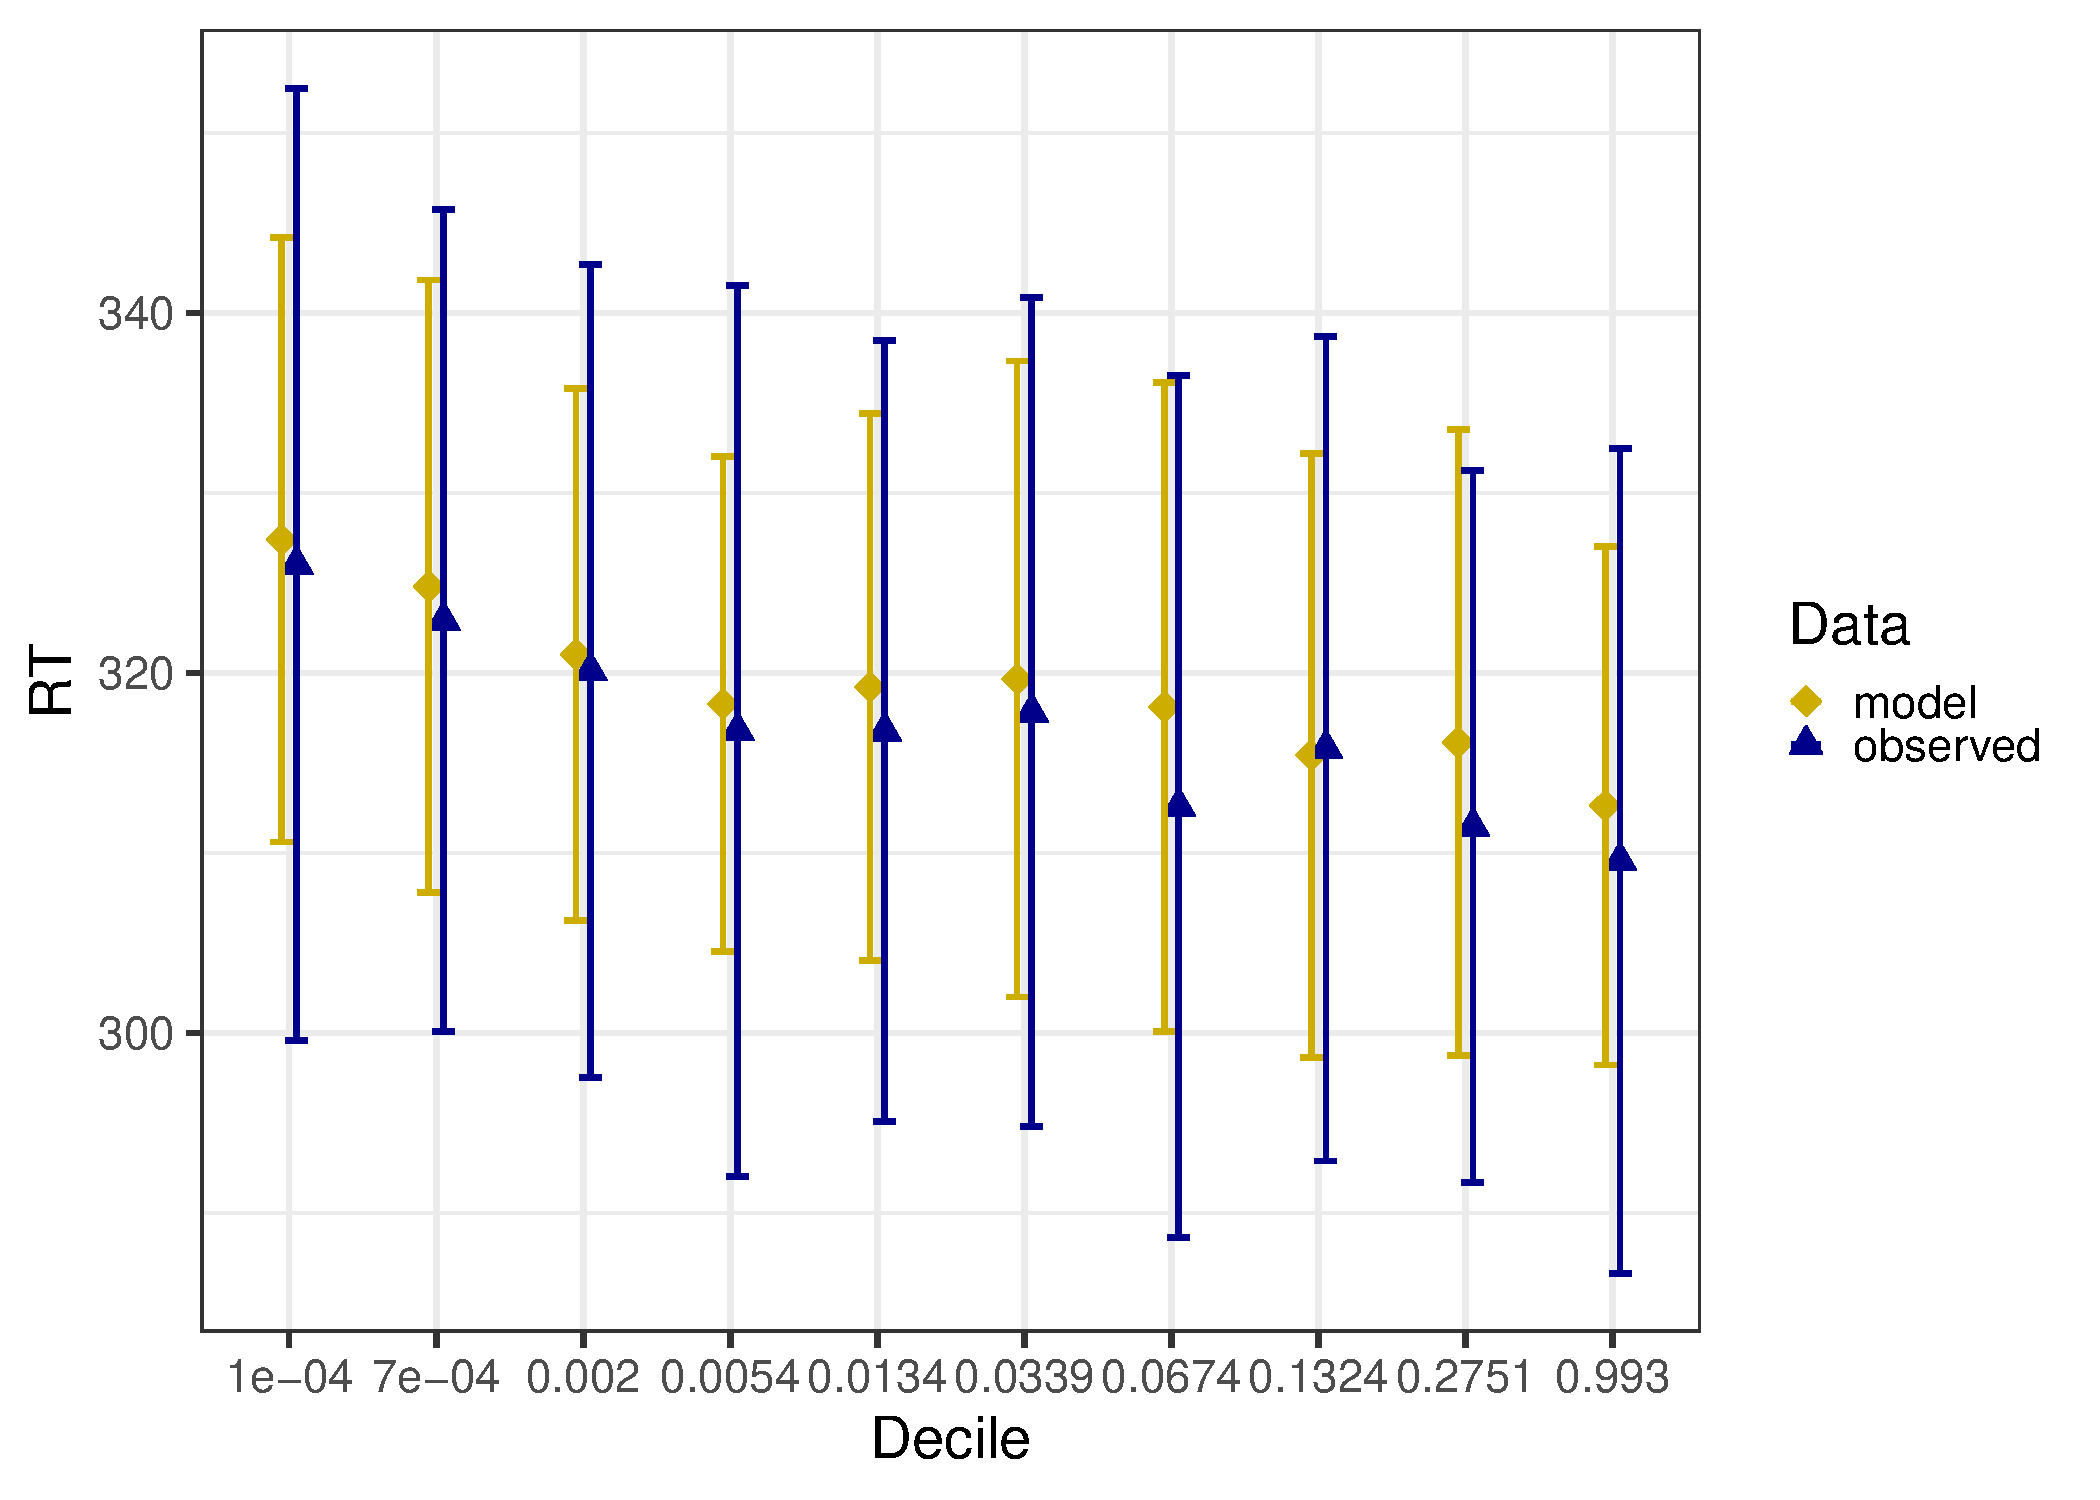
\includegraphics[width=\maxwidth]{figures/figure_ns_unnamed-chunk-11-1} 

\end{knitrout}

\begin{knitrout}
\definecolor{shadecolor}{rgb}{0.969, 0.969, 0.969}\color{fgcolor}\begin{kframe}
\begin{alltt}
\hlkwd{ggsave}\hlstd{(}\hlstr{"trigrams.png"}\hlstd{,} \hlkwc{width} \hlstd{=} \hlnum{19}\hlstd{,} \hlkwc{height} \hlstd{=} \hlnum{12}\hlstd{)}
\end{alltt}
\end{kframe}
\end{knitrout}

\begin{knitrout}
\definecolor{shadecolor}{rgb}{0.969, 0.969, 0.969}\color{fgcolor}\begin{kframe}
\begin{alltt}
\hlstd{cutoff} \hlkwb{<-} \hlkwd{quantile}\hlstd{(sumdata}\hlopt{$}\hlstd{Freq,} \hlkwd{seq}\hlstd{(}\hlnum{0}\hlstd{,} \hlnum{1}\hlstd{,} \hlnum{0.1}\hlstd{))}

\hlstd{cutoff}
\end{alltt}
\begin{verbatim}
##         0%        10%        20%        30%        40%        50% 
##      31747    1999559    8835068   32601982   91027817  242417228 
##        60%        70%        80%        90%       100% 
##  599554050 1140172617 4223327232 9819942513 9819942513
\end{verbatim}
\begin{alltt}
\hlkwd{subset}\hlstd{(sumdata, Freq} \hlopt{>=} \hlnum{9.81e+09}\hlstd{)}
\end{alltt}
\begin{verbatim}
## # A tibble: 133 x 13
##    Item  Region    RT Position   Freq Bigram Trigram Observed Sentence_no
##    <fct> <fct>  <dbl>    <int>  <dbl>  <dbl>   <dbl>    <dbl>       <dbl>
##  1 1     No_00~  305.        7 9.82e9 0.0907  0.0674     298.           1
##  2 1     No_00~  305.       16 9.82e9 0.129   0.184      321.           1
##  3 1     No_00~  305.        3 9.82e9 0.0521  0.0691     310.           2
##  4 1     No_00~  305.        8 9.82e9 0.0752  0.0583     294.           2
##  5 1     No_00~  305.       25 9.82e9 0.0907  0.0801     295.           2
##  6 1     No_00~  305.        2 9.82e9 0.236   0.244      331.           3
##  7 1     No_00~  305.        9 9.82e9 0.0767  0.0857     355.           3
##  8 1     No_00~  305.       12 9.82e9 0.250   0.120      307.           3
##  9 1     No_00~  305.       11 9.82e9 0.274   0.934      299.           4
## 10 1     No_00~  305.       15 9.82e9 0.0142  0.0388     302            4
## # ... with 123 more rows, and 4 more variables: Word <chr>, Nchar <int>,
## #   Absolute_position <dbl>, Trigramcat <fct>
\end{verbatim}
\begin{alltt}
\hlkwd{subset}\hlstd{(sumdata, Word} \hlopt{==} \hlstr{"the"}\hlstd{)}
\end{alltt}
\begin{verbatim}
## # A tibble: 133 x 13
##    Item  Region    RT Position   Freq Bigram Trigram Observed Sentence_no
##    <fct> <fct>  <dbl>    <int>  <dbl>  <dbl>   <dbl>    <dbl>       <dbl>
##  1 1     No_00~  305.        7 9.82e9 0.0907  0.0674     298.           1
##  2 1     No_00~  305.       16 9.82e9 0.129   0.184      321.           1
##  3 1     No_00~  305.        3 9.82e9 0.0521  0.0691     310.           2
##  4 1     No_00~  305.        8 9.82e9 0.0752  0.0583     294.           2
##  5 1     No_00~  305.       25 9.82e9 0.0907  0.0801     295.           2
##  6 1     No_00~  305.        2 9.82e9 0.236   0.244      331.           3
##  7 1     No_00~  305.        9 9.82e9 0.0767  0.0857     355.           3
##  8 1     No_00~  305.       12 9.82e9 0.250   0.120      307.           3
##  9 1     No_00~  305.       11 9.82e9 0.274   0.934      299.           4
## 10 1     No_00~  305.       15 9.82e9 0.0142  0.0388     302            4
## # ... with 123 more rows, and 4 more variables: Word <chr>, Nchar <int>,
## #   Absolute_position <dbl>, Trigramcat <fct>
\end{verbatim}
\begin{alltt}
\hlcom{# cutoff[10] <- cutoff[10]-1 #we do this because just one word (the)}
\hlcom{# occupies more than one quantile and if we did not do it, the last two}
\hlcom{# quantiles would be identical}

\hlkwd{str}\hlstd{(sumdata)}
\end{alltt}
\begin{verbatim}
## tibble [1,140 x 13] (S3: tbl_df/tbl/data.frame)
##  $ Item             : Factor w/ 2 levels "1","2": 1 1 1 1 1 1 1 1 1 1 ...
##  $ Region           : Factor w/ 1312 levels "No_0001","No_0002",..: 1 2 3 4 5 6 7 8 10 11 ...
##  $ RT               : num [1:1140] 307 339 351 307 317 ...
##  $ Position         : int [1:1140] 2 3 4 5 6 7 8 9 11 12 ...
##  $ Freq             : num [1:1140] 1.72e+08 1.75e+09 1.32e+06 2.06e+08 7.60e+06 ...
##  $ Bigram           : num [1:1140] 1.84e-02 6.00e-02 8.99e-05 5.30e-03 7.02e-04 ...
##  $ Trigram          : num [1:1140] 0.018117 0.152912 0.000334 0.009856 0.003151 ...
##  $ Observed         : num [1:1140] 313 307 338 308 311 ...
##  $ Sentence_no      : num [1:1140] 1 1 1 1 1 1 1 1 1 1 ...
##  $ Word             : chr [1:1140] "said" "that" "whoever" "could" ...
##  $ Nchar            : int [1:1140] 4 4 7 5 4 3 4 3 2 5 ...
##  $ Absolute_position: num [1:1140] 1 2 3 4 5 6 7 8 10 11 ...
##  $ Trigramcat       : Factor w/ 10 levels "0.1","0.2","0.3",..: 6 9 2 5 4 7 2 7 2 4 ...
\end{verbatim}
\begin{alltt}
\hlstd{sumdata}\hlopt{$}\hlstd{Freqcat} \hlkwb{<-} \hlkwd{cut}\hlstd{(sumdata}\hlopt{$}\hlstd{Freq,} \hlkwc{breaks} \hlstd{= cutoff[}\hlnum{1}\hlopt{:}\hlnum{10}\hlstd{],} \hlkwc{labels} \hlstd{=} \hlkwd{seq}\hlstd{(}\hlnum{0.1}\hlstd{,}
    \hlnum{1}\hlstd{,} \hlnum{0.1}\hlstd{)[}\hlnum{1}\hlopt{:}\hlnum{9}\hlstd{])}

\hlstd{sumdata} \hlkwb{<-} \hlkwd{subset}\hlstd{(sumdata,} \hlopt{!}\hlkwd{is.na}\hlstd{(Freqcat))}

\hlstd{summary.Freq} \hlkwb{<-} \hlstd{sumdata} \hlopt \hlkwd{group_by}\hlstd{(Freqcat)} \hlopt \hlkwd{summarise}\hlstd{(}\hlkwc{Predicted} \hlstd{=} \hlkwd{median}\hlstd{(RT),}
    \hlkwc{sdPredicted} \hlstd{=} \hlkwd{sd}\hlstd{(RT),} \hlkwc{Found} \hlstd{=} \hlkwd{median}\hlstd{(Observed),} \hlkwc{sdFound} \hlstd{=} \hlkwd{sd}\hlstd{(Observed),}
    \hlkwc{count} \hlstd{=} \hlkwd{length}\hlstd{(Observed))}

\hlstd{summary.Freq}
\end{alltt}
\begin{verbatim}
## # A tibble: 9 x 6
##   Freqcat Predicted sdPredicted Found sdFound count
## * <fct>       <dbl>       <dbl> <dbl>   <dbl> <int>
## 1 0.1          325.        15.9  324.    26.8   114
## 2 0.2          321.        14.1  319.    23.6   113
## 3 0.3          315.        11.5  317.    22.5   114
## 4 0.4          310.        13.7  313.    23.0   114
## 5 0.5          308.        12.2  309.    19.5   115
## 6 0.6          307.        22.1  317.    21.8   114
## 7 0.7          306.        15.2  315.    20.9   141
## 8 0.8          306.        19.6  309.    25.7   102
## 9 0.9          305.        15.5  308.    23.7   212
\end{verbatim}
\begin{alltt}
\hlstd{summary.Freq}\hlopt{$}\hlstd{Freqcat} \hlkwb{<-} \hlkwd{as.character}\hlstd{(summary.Freq}\hlopt{$}\hlstd{Freqcat)}

\hlstd{summary.Freq}\hlopt{$}\hlstd{Freqcat} \hlkwb{<-} \hlkwd{round}\hlstd{(}\hlkwd{log}\hlstd{(cutoff[}\hlnum{2}\hlopt{:}\hlnum{10}\hlstd{]),} \hlnum{3}\hlstd{)}

\hlstd{summary.Freq}\hlopt{$}\hlstd{Freqcat} \hlkwb{<-} \hlkwd{as.factor}\hlstd{(summary.Freq}\hlopt{$}\hlstd{Freqcat)}

\hlstd{data.to.plot} \hlkwb{<-} \hlkwd{data.frame}\hlstd{(}\hlkwc{Decile_values_in_log} \hlstd{=} \hlkwd{as.factor}\hlstd{(}\hlkwd{rep}\hlstd{(summary.Freq}\hlopt{$}\hlstd{Freqcat,}
    \hlnum{2}\hlstd{)),} \hlkwc{RT} \hlstd{=} \hlkwd{c}\hlstd{(summary.Freq}\hlopt{$}\hlstd{Predicted, summary.Freq}\hlopt{$}\hlstd{Found),} \hlkwc{std} \hlstd{=} \hlkwd{c}\hlstd{(summary.Freq}\hlopt{$}\hlstd{sdPredicted,}
    \hlstd{summary.Freq}\hlopt{$}\hlstd{sdFound),} \hlkwc{Data} \hlstd{=} \hlkwd{c}\hlstd{(}\hlkwd{rep}\hlstd{(}\hlstr{"model"}\hlstd{,} \hlnum{9}\hlstd{),} \hlkwd{rep}\hlstd{(}\hlstr{"observed"}\hlstd{,} \hlnum{9}\hlstd{)))}

\hlkwd{library}\hlstd{(ggplot2)}

\hlkwd{library}\hlstd{(dplyr)}

\hlstd{g1} \hlkwb{<-} \hlkwd{ggplot}\hlstd{(data.to.plot,} \hlkwd{aes}\hlstd{(Decile_values_in_log, RT,} \hlkwc{color} \hlstd{= Data,} \hlkwc{fill} \hlstd{= Data,}
    \hlkwc{pch} \hlstd{= Data))}
\hlstd{g1} \hlkwb{<-} \hlstd{g1} \hlopt{+} \hlkwd{geom_point}\hlstd{(}\hlkwc{position} \hlstd{= dodge,} \hlkwc{size} \hlstd{=} \hlkwd{I}\hlstd{(}\hlnum{5}\hlstd{))} \hlopt{+} \hlkwd{geom_errorbar}\hlstd{(}\hlkwd{aes}\hlstd{(}\hlkwc{ymin} \hlstd{= RT} \hlopt{-}
    \hlstd{std,} \hlkwc{ymax} \hlstd{= RT} \hlopt{+} \hlstd{std),} \hlkwc{position} \hlstd{= dodge,} \hlkwc{width} \hlstd{=} \hlnum{0.3}\hlstd{,} \hlkwc{size} \hlstd{=} \hlkwd{I}\hlstd{(}\hlnum{1.3}\hlstd{))} \hlopt{+}
    \hlkwd{scale_shape_manual}\hlstd{(}\hlkwc{values} \hlstd{=} \hlnum{23}\hlopt{:}\hlnum{24}\hlstd{)} \hlopt{+} \hlkwd{scale_color_manual}\hlstd{(}\hlkwc{values} \hlstd{=} \hlkwd{c}\hlstd{(}\hlstr{"gold3"}\hlstd{,}
    \hlstr{"blue4"}\hlstd{))} \hlopt{+} \hlkwd{scale_fill_manual}\hlstd{(}\hlkwc{values} \hlstd{=} \hlkwd{c}\hlstd{(}\hlstr{"gold3"}\hlstd{,} \hlstr{"blue4"}\hlstd{))} \hlopt{+} \hlkwd{theme_bw}\hlstd{(}\hlnum{28}\hlstd{)}
\end{alltt}
\end{kframe}
\end{knitrout}
\begin{knitrout}
\definecolor{shadecolor}{rgb}{0.969, 0.969, 0.969}\color{fgcolor}
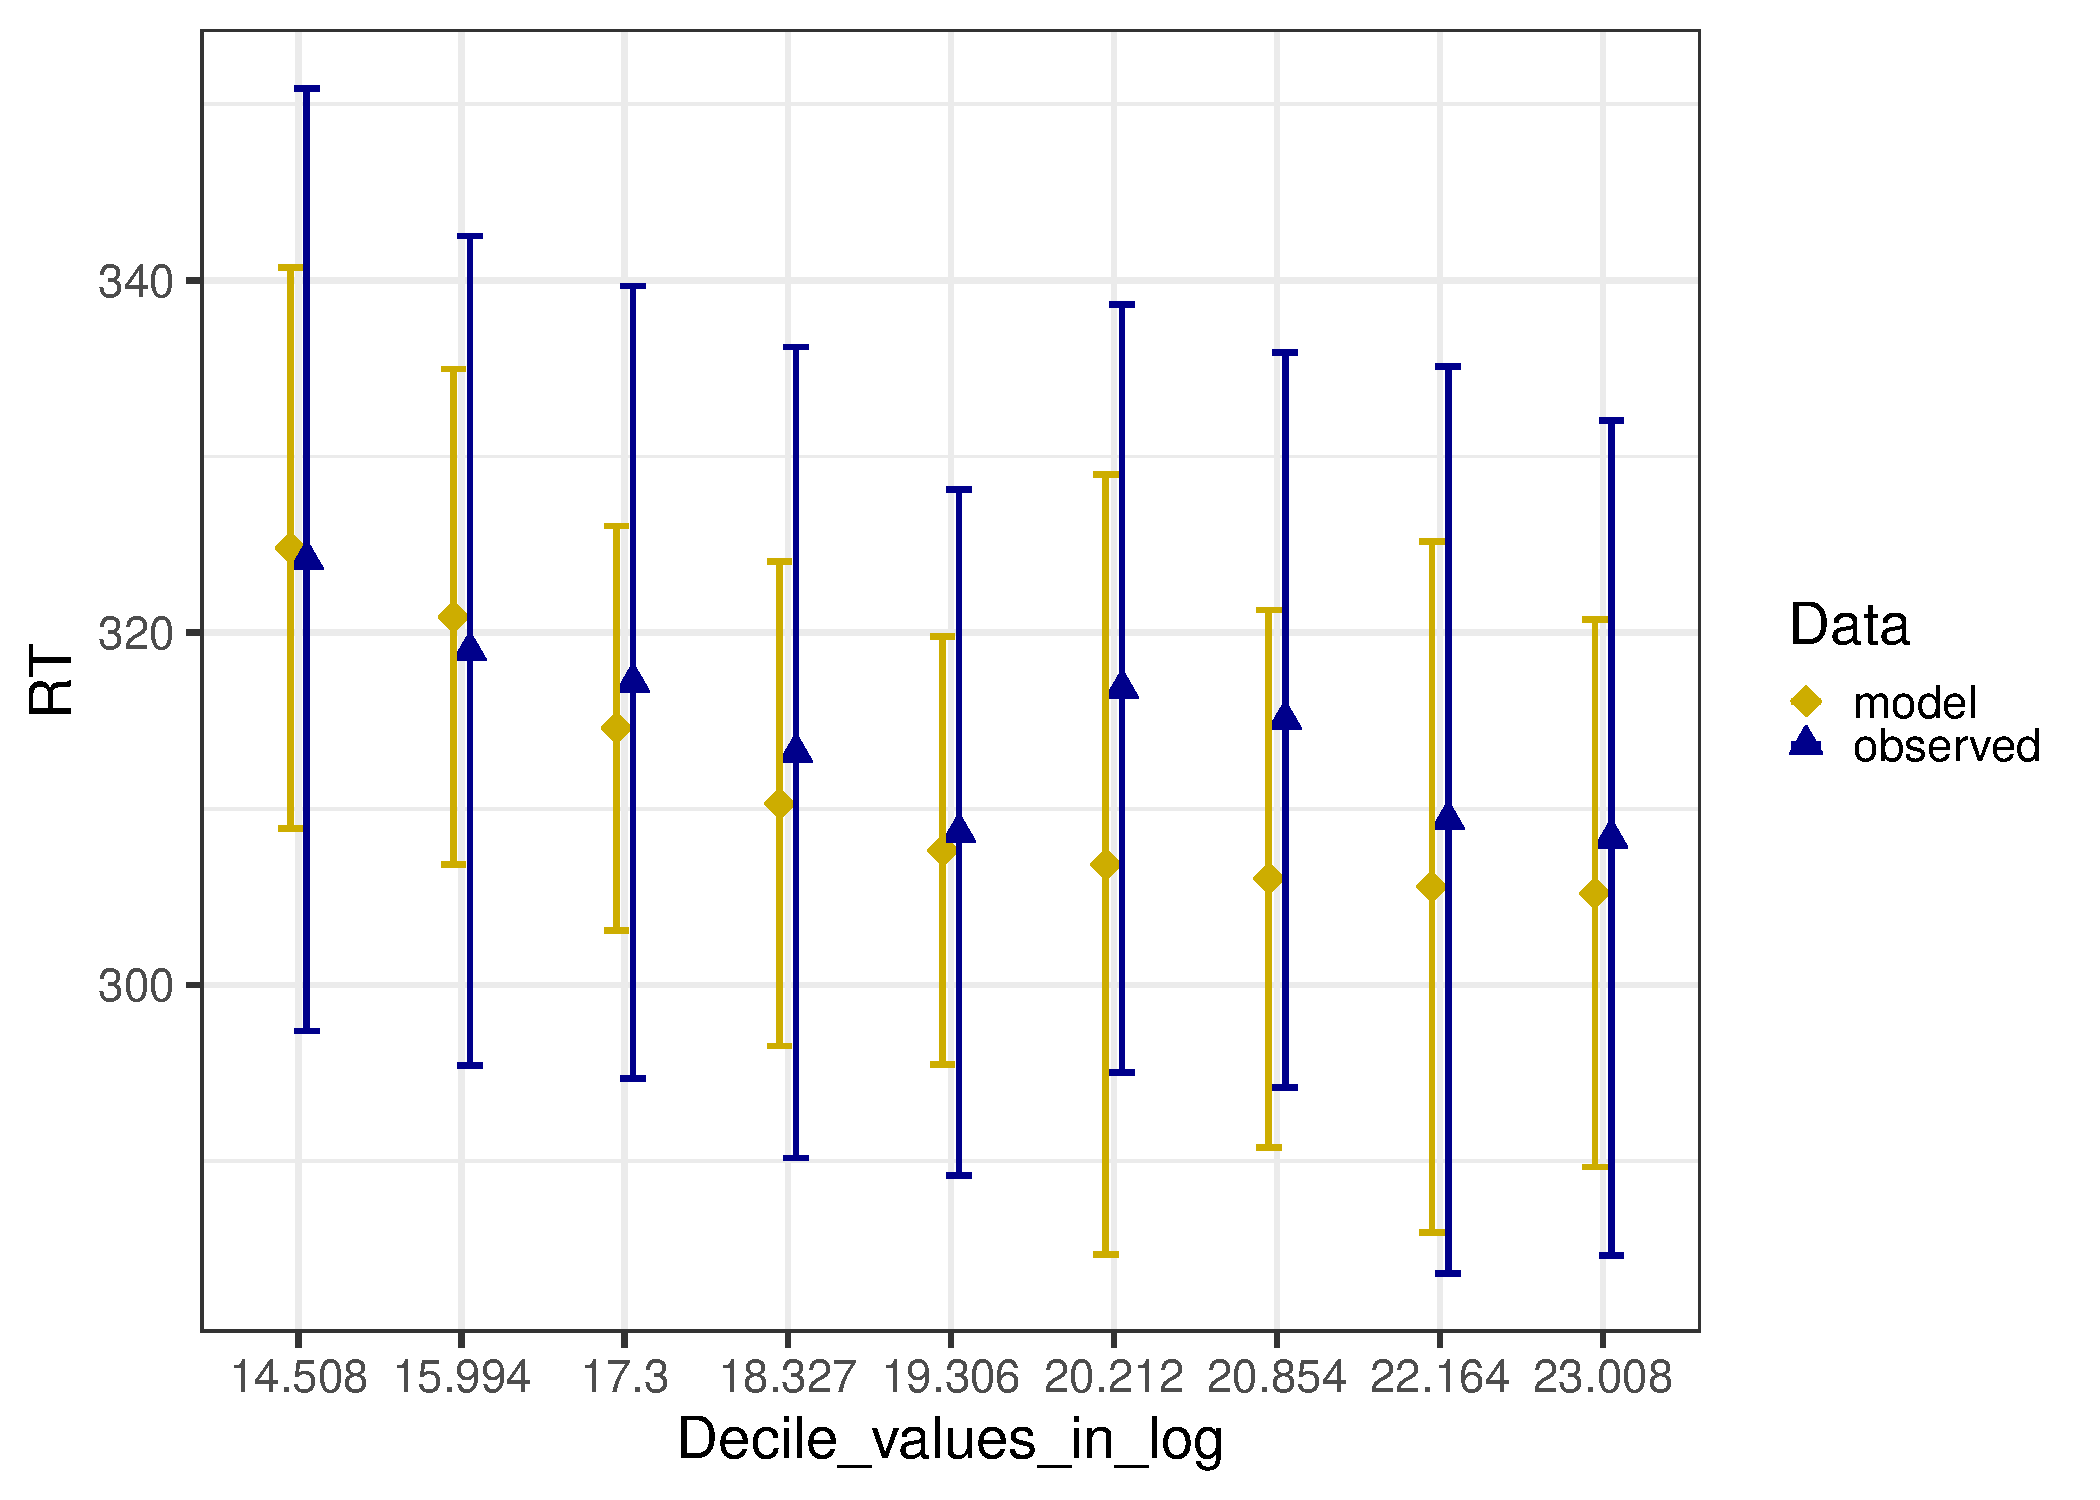
\includegraphics[width=\maxwidth]{figures/figure_ns_unnamed-chunk-14-1} 

\end{knitrout}

\begin{knitrout}
\definecolor{shadecolor}{rgb}{0.969, 0.969, 0.969}\color{fgcolor}\begin{kframe}
\begin{alltt}
\hlkwd{ggsave}\hlstd{(}\hlstr{"freqs.png"}\hlstd{,} \hlkwc{width} \hlstd{=} \hlnum{19}\hlstd{,} \hlkwc{height} \hlstd{=} \hlnum{12}\hlstd{)}
\end{alltt}
\end{kframe}
\end{knitrout}

\begin{knitrout}
\definecolor{shadecolor}{rgb}{0.969, 0.969, 0.969}\color{fgcolor}\begin{kframe}
\begin{alltt}
\hlstd{cutoff} \hlkwb{<-} \hlkwd{quantile}\hlstd{(sumdata}\hlopt{$}\hlstd{RT,} \hlkwd{seq}\hlstd{(}\hlnum{0}\hlstd{,} \hlnum{1}\hlstd{,} \hlnum{0.1}\hlstd{))}

\hlstd{cutoff}
\end{alltt}
\begin{verbatim}
##       0%      10%      20%      30%      40%      50%      60%      70% 
## 305.2119 305.2129 305.7162 306.1664 307.9639 311.6690 316.8998 323.8358 
##      80%      90%     100% 
## 338.3626 339.8425 397.1125
\end{verbatim}
\begin{alltt}
\hlstd{sumdata}\hlopt{$}\hlstd{RTcat} \hlkwb{<-} \hlkwd{cut}\hlstd{(sumdata}\hlopt{$}\hlstd{RT,} \hlkwc{breaks} \hlstd{= cutoff,} \hlkwc{labels} \hlstd{=} \hlkwd{seq}\hlstd{(}\hlnum{0.1}\hlstd{,} \hlnum{1}\hlstd{,} \hlnum{0.1}\hlstd{))}

\hlstd{sumdata} \hlkwb{<-} \hlkwd{subset}\hlstd{(sumdata,} \hlopt{!}\hlkwd{is.na}\hlstd{(RTcat))}

\hlstd{summary.RT} \hlkwb{<-} \hlstd{sumdata} \hlopt \hlkwd{group_by}\hlstd{(RTcat)} \hlopt \hlkwd{summarise}\hlstd{(}\hlkwc{Predicted} \hlstd{=} \hlkwd{mean}\hlstd{(RT),}
    \hlkwc{sdPredicted} \hlstd{=} \hlkwd{sd}\hlstd{(RT),} \hlkwc{Found} \hlstd{=} \hlkwd{mean}\hlstd{(Observed),} \hlkwc{sdFound} \hlstd{=} \hlkwd{sd}\hlstd{(Observed))}

\hlstd{summary.RT}
\end{alltt}
\begin{verbatim}
## # A tibble: 10 x 5
##    RTcat Predicted sdPredicted Found sdFound
##  * <fct>     <dbl>       <dbl> <dbl>   <dbl>
##  1 0.1        305.    0.000310  311.    22.6
##  2 0.2        305.    0.127     312.    24.2
##  3 0.3        306.    0.159     317.    21.9
##  4 0.4        307.    0.464     310.    18.7
##  5 0.5        310.    1.03      314.    21.1
##  6 0.6        314.    1.65      319.    23.5
##  7 0.7        320.    1.98      322.    22.8
##  8 0.8        332.    5.81      322.    25.9
##  9 0.9        339.    0.442     316.    23.5
## 10 1          353.   13.7       326.    25.8
\end{verbatim}
\begin{alltt}
\hlkwd{cor.test}\hlstd{(summary.RT}\hlopt{$}\hlstd{Predicted, summary.RT}\hlopt{$}\hlstd{Found)}
\end{alltt}
\begin{verbatim}
## 
## 	Pearson's product-moment correlation
## 
## data:  summary.RT$Predicted and summary.RT$Found
## t = 3.4725, df = 8, p-value = 0.008412
## alternative hypothesis: true correlation is not equal to 0
## 95 percent confidence interval:
##  0.2847095 0.9440889
## sample estimates:
##       cor 
## 0.7753467
\end{verbatim}
\begin{alltt}
\hlstd{data.to.plot} \hlkwb{<-} \hlkwd{data.frame}\hlstd{(}\hlkwc{Decile} \hlstd{=} \hlkwd{rep}\hlstd{(summary.RT}\hlopt{$}\hlstd{RTcat,} \hlnum{2}\hlstd{),} \hlkwc{RT} \hlstd{=} \hlkwd{c}\hlstd{(summary.RT}\hlopt{$}\hlstd{Predicted,}
    \hlstd{summary.RT}\hlopt{$}\hlstd{Found),} \hlkwc{std} \hlstd{=} \hlkwd{c}\hlstd{(summary.RT}\hlopt{$}\hlstd{sdPredicted, summary.RT}\hlopt{$}\hlstd{sdFound),}
    \hlkwc{Data} \hlstd{=} \hlkwd{c}\hlstd{(}\hlkwd{rep}\hlstd{(}\hlstr{"model"}\hlstd{,} \hlnum{10}\hlstd{),} \hlkwd{rep}\hlstd{(}\hlstr{"observed"}\hlstd{,} \hlnum{10}\hlstd{)))}

\hlkwd{library}\hlstd{(ggplot2)}

\hlkwd{library}\hlstd{(dplyr)}

\hlstd{g1} \hlkwb{<-} \hlkwd{ggplot}\hlstd{(data.to.plot,} \hlkwd{aes}\hlstd{(Decile, RT,} \hlkwc{color} \hlstd{= Data,} \hlkwc{fill} \hlstd{= Data,} \hlkwc{pch} \hlstd{= Data))}
\hlstd{g1} \hlkwb{<-} \hlstd{g1} \hlopt{+} \hlkwd{geom_point}\hlstd{(}\hlkwc{position} \hlstd{= dodge,} \hlkwc{size} \hlstd{=} \hlkwd{I}\hlstd{(}\hlnum{5}\hlstd{))} \hlopt{+} \hlkwd{geom_errorbar}\hlstd{(}\hlkwd{aes}\hlstd{(}\hlkwc{ymin} \hlstd{= RT} \hlopt{-}
    \hlstd{std,} \hlkwc{ymax} \hlstd{= RT} \hlopt{+} \hlstd{std),} \hlkwc{position} \hlstd{= dodge,} \hlkwc{width} \hlstd{=} \hlnum{0.3}\hlstd{,} \hlkwc{size} \hlstd{=} \hlkwd{I}\hlstd{(}\hlnum{1.3}\hlstd{))} \hlopt{+}
    \hlkwd{scale_shape_manual}\hlstd{(}\hlkwc{values} \hlstd{=} \hlnum{23}\hlopt{:}\hlnum{24}\hlstd{)} \hlopt{+} \hlkwd{scale_color_manual}\hlstd{(}\hlkwc{values} \hlstd{=} \hlkwd{c}\hlstd{(}\hlstr{"gold3"}\hlstd{,}
    \hlstr{"blue4"}\hlstd{))} \hlopt{+} \hlkwd{scale_fill_manual}\hlstd{(}\hlkwc{values} \hlstd{=} \hlkwd{c}\hlstd{(}\hlstr{"gold3"}\hlstd{,} \hlstr{"blue4"}\hlstd{))} \hlopt{+} \hlkwd{theme_bw}\hlstd{(}\hlnum{28}\hlstd{)}
\end{alltt}
\end{kframe}
\end{knitrout}
\begin{knitrout}
\definecolor{shadecolor}{rgb}{0.969, 0.969, 0.969}\color{fgcolor}
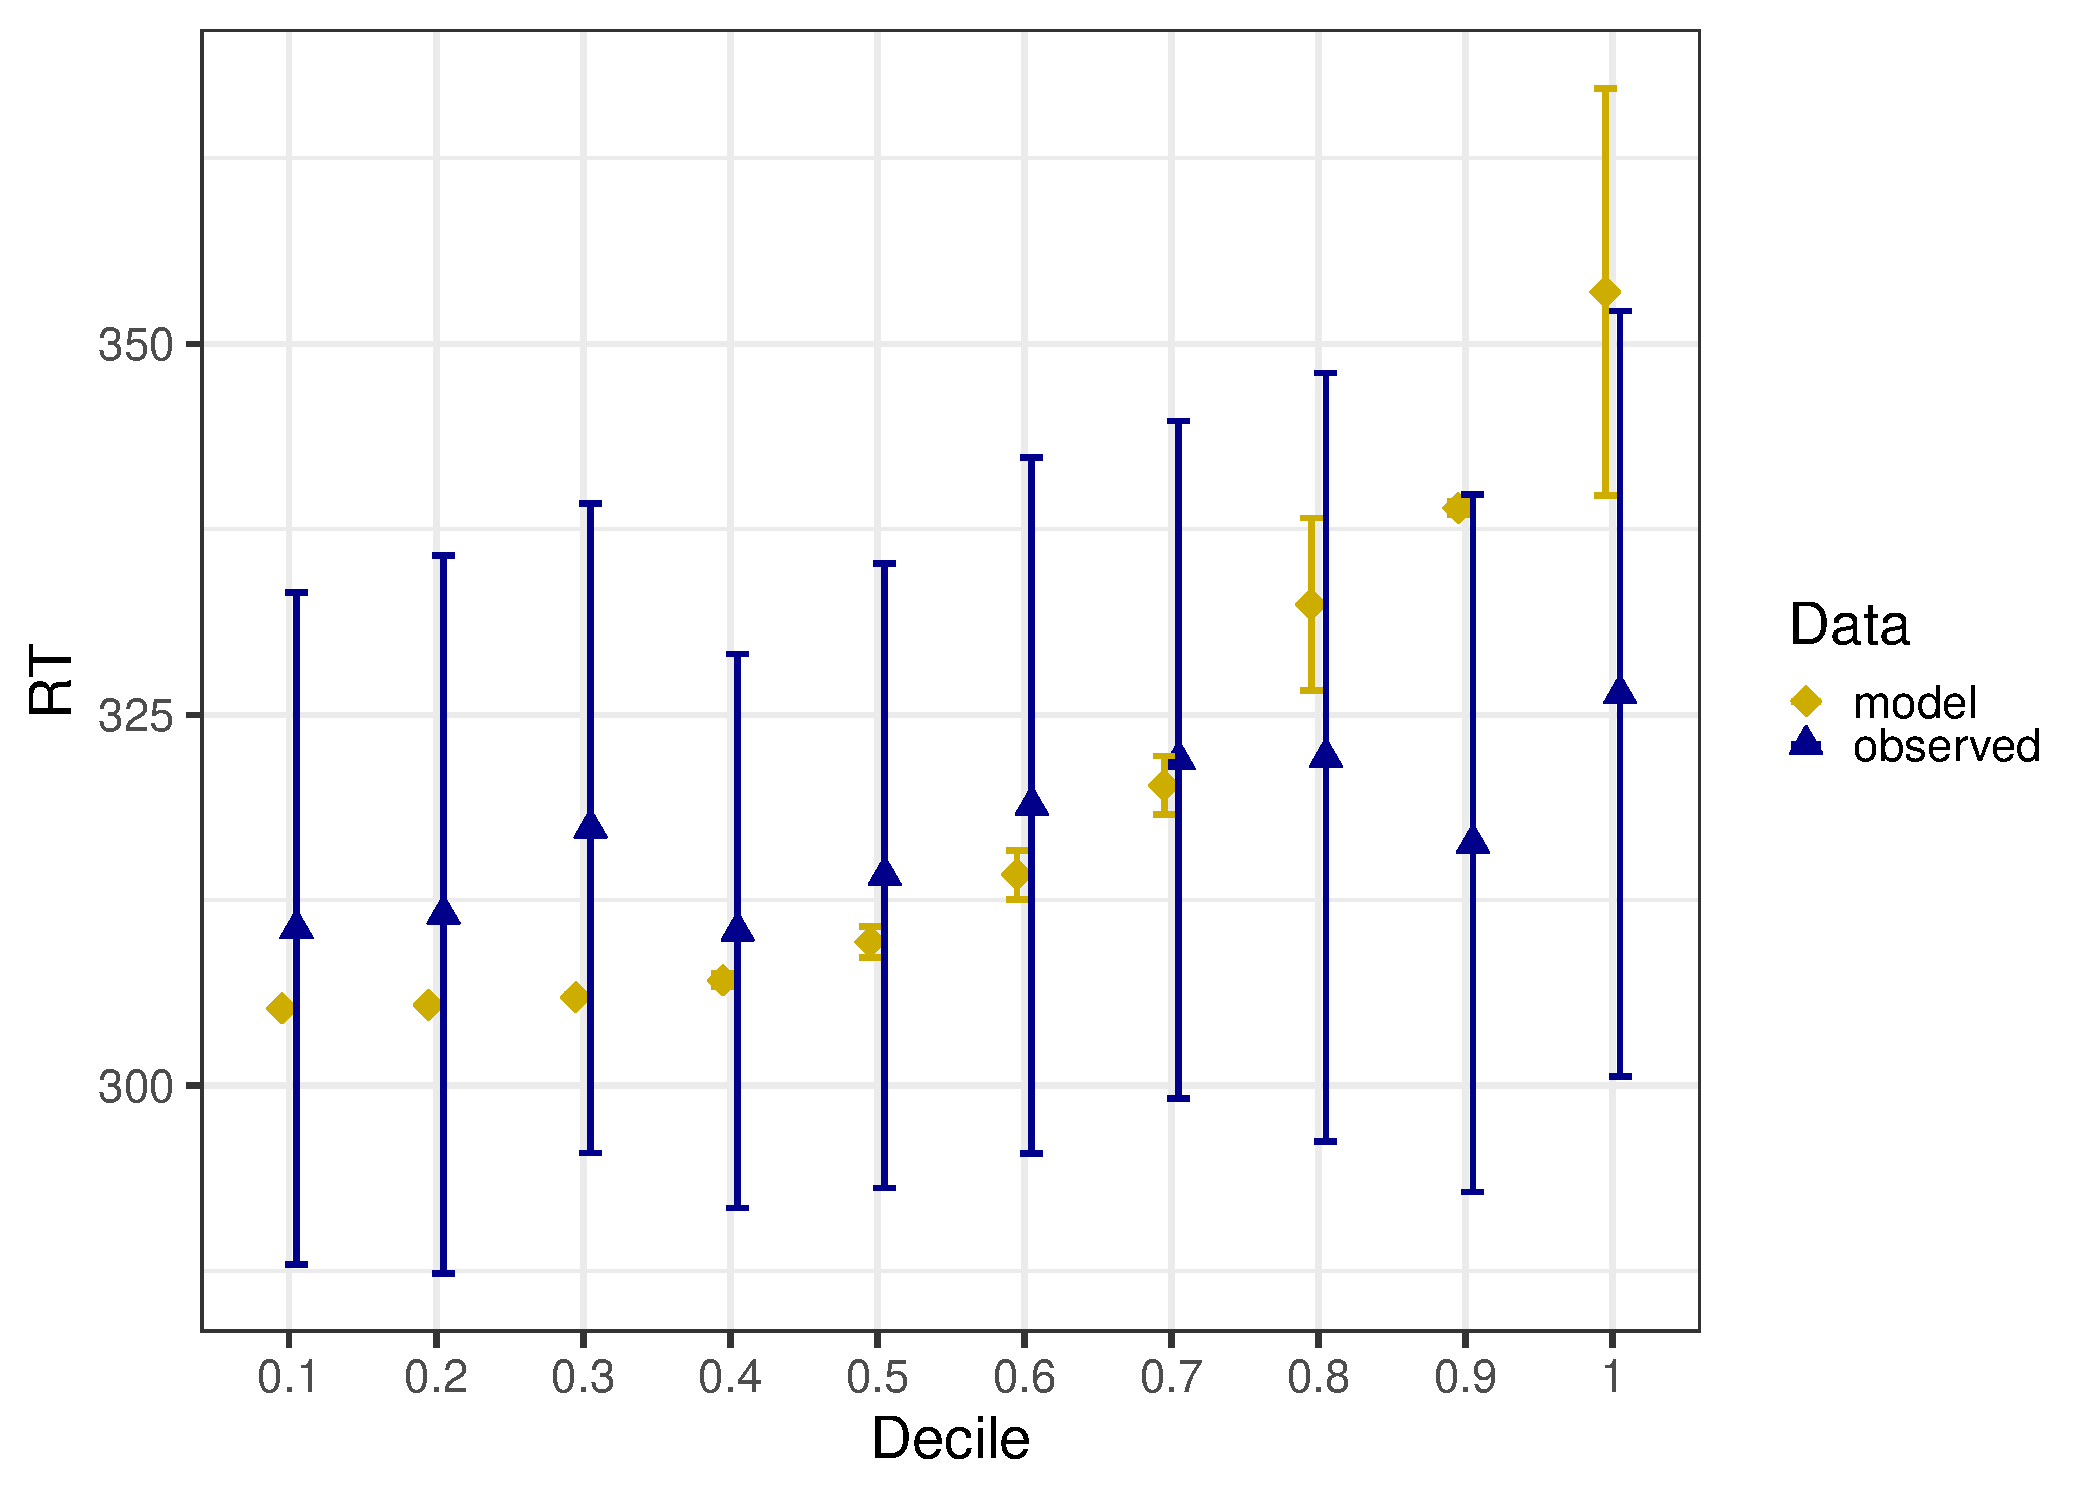
\includegraphics[width=\maxwidth]{figures/figure_ns_unnamed-chunk-17-1} 

\end{knitrout}

\begin{knitrout}
\definecolor{shadecolor}{rgb}{0.969, 0.969, 0.969}\color{fgcolor}\begin{kframe}
\begin{alltt}
\hlstd{cutoff} \hlkwb{<-} \hlkwd{quantile}\hlstd{(sumdata}\hlopt{$}\hlstd{Observed,} \hlkwd{seq}\hlstd{(}\hlnum{0}\hlstd{,} \hlnum{1}\hlstd{,} \hlnum{0.1}\hlstd{))}

\hlstd{sumdata}\hlopt{$}\hlstd{Observedcat} \hlkwb{<-} \hlkwd{cut}\hlstd{(sumdata}\hlopt{$}\hlstd{Observed,} \hlkwc{breaks} \hlstd{= cutoff,} \hlkwc{labels} \hlstd{=} \hlkwd{seq}\hlstd{(}\hlnum{0.1}\hlstd{,}
    \hlnum{1}\hlstd{,} \hlnum{0.1}\hlstd{))}

\hlstd{sumdata} \hlkwb{<-} \hlkwd{subset}\hlstd{(sumdata,} \hlopt{!}\hlkwd{is.na}\hlstd{(Observedcat))}

\hlstd{summary.Observed} \hlkwb{<-} \hlstd{sumdata} \hlopt \hlkwd{group_by}\hlstd{(Observedcat)} \hlopt \hlkwd{summarise}\hlstd{(}\hlkwc{Predicted} \hlstd{=} \hlkwd{mean}\hlstd{(RT),}
    \hlkwc{sdPredicted} \hlstd{=} \hlkwd{sd}\hlstd{(RT),} \hlkwc{Found} \hlstd{=} \hlkwd{mean}\hlstd{(Observed),} \hlkwc{sdFound} \hlstd{=} \hlkwd{sd}\hlstd{(Observed))}

\hlstd{summary.Observed}
\end{alltt}
\begin{verbatim}
## # A tibble: 10 x 5
##    Observedcat Predicted sdPredicted Found sdFound
##  * <fct>           <dbl>       <dbl> <dbl>   <dbl>
##  1 0.1              316.        14.3  284.    5.01
##  2 0.2              316.        15.1  294.    2.22
##  3 0.3              318.        16.3  300.    1.98
##  4 0.4              316.        16.0  307.    1.44
##  5 0.5              320.        16.9  311.    1.60
##  6 0.6              321.        17.5  317.    1.41
##  7 0.7              318.        17.3  322.    1.84
##  8 0.8              320.        15.1  330.    2.65
##  9 0.9              322.        17.4  340.    3.25
## 10 1                325.        18.8  365.   19.5
\end{verbatim}
\begin{alltt}
\hlkwd{cor.test}\hlstd{(summary.Observed}\hlopt{$}\hlstd{Predicted, summary.Observed}\hlopt{$}\hlstd{Found)}
\end{alltt}
\begin{verbatim}
## 
## 	Pearson's product-moment correlation
## 
## data:  summary.Observed$Predicted and summary.Observed$Found
## t = 5.7946, df = 8, p-value = 0.0004077
## alternative hypothesis: true correlation is not equal to 0
## 95 percent confidence interval:
##  0.6196320 0.9760291
## sample estimates:
##       cor 
## 0.8986587
\end{verbatim}
\begin{alltt}
\hlstd{m1} \hlkwb{<-} \hlkwd{lm}\hlstd{(summary.Observed}\hlopt{$}\hlstd{Predicted} \hlopt{~ -}\hlnum{1} \hlopt{+} \hlstd{summary.Observed}\hlopt{$}\hlstd{Found)}
\hlkwd{summary}\hlstd{(m1)}
\end{alltt}
\begin{verbatim}
## 
## Call:
## lm(formula = summary.Observed$Predicted ~ -1 + summary.Observed$Found)
## 
## Residuals:
##     Min      1Q  Median      3Q     Max 
## -40.560  -9.325   5.771  15.032  31.310 
## 
## Coefficients:
##                        Estimate Std. Error t value Pr(>|t|)    
## summary.Observed$Found   1.0026     0.0211   47.52 4.06e-12 ***
## ---
## Signif. codes:  0 '***' 0.001 '**' 0.01 '*' 0.05 '.' 0.1 ' ' 1
## 
## Residual standard error: 21.21 on 9 degrees of freedom
## Multiple R-squared:  0.996,	Adjusted R-squared:  0.9956 
## F-statistic:  2258 on 1 and 9 DF,  p-value: 4.058e-12
\end{verbatim}
\begin{alltt}
\hlstd{summary.Observed}\hlopt{$}\hlstd{Observedcat} \hlkwb{<-} \hlkwd{as.character}\hlstd{(summary.Observed}\hlopt{$}\hlstd{Observedcat)}

\hlstd{summary.Observed}\hlopt{$}\hlstd{Observedcat} \hlkwb{<-} \hlkwd{round}\hlstd{(cutoff[}\hlnum{2}\hlopt{:}\hlnum{11}\hlstd{])}

\hlstd{summary.Observed}\hlopt{$}\hlstd{Observedcat} \hlkwb{<-} \hlkwd{as.factor}\hlstd{(summary.Observed}\hlopt{$}\hlstd{Observedcat)}


\hlstd{data.to.plot} \hlkwb{<-} \hlkwd{data.frame}\hlstd{(}\hlkwc{Decile} \hlstd{=} \hlkwd{rep}\hlstd{(summary.Observed}\hlopt{$}\hlstd{Observedcat,} \hlnum{2}\hlstd{),} \hlkwc{RT} \hlstd{=} \hlkwd{c}\hlstd{(summary.Observed}\hlopt{$}\hlstd{Predicted,}
    \hlstd{summary.Observed}\hlopt{$}\hlstd{Found),} \hlkwc{std} \hlstd{=} \hlkwd{c}\hlstd{(summary.Observed}\hlopt{$}\hlstd{sdPredicted, summary.Observed}\hlopt{$}\hlstd{sdFound),}
    \hlkwc{Data} \hlstd{=} \hlkwd{c}\hlstd{(}\hlkwd{rep}\hlstd{(}\hlstr{"model"}\hlstd{,} \hlnum{10}\hlstd{),} \hlkwd{rep}\hlstd{(}\hlstr{"observed"}\hlstd{,} \hlnum{10}\hlstd{)))}

\hlstd{data.to.plot}
\end{alltt}
\begin{verbatim}
##    Decile       RT       std     Data
## 1     290 315.7072 14.259645    model
## 2     297 315.8985 15.111654    model
## 3     304 318.1744 16.327556    model
## 4     309 316.3260 16.045432    model
## 5     314 320.1699 16.935492    model
## 6     319 321.4270 17.458987    model
## 7     326 317.7947 17.258142    model
## 8     335 320.3360 15.076059    model
## 9     346 321.7311 17.391639    model
## 10    440 325.1657 18.816902    model
## 11    290 283.6501  5.007106 observed
## 12    297 293.7607  2.220551 observed
## 13    304 300.3326  1.976318 observed
## 14    309 306.5420  1.442146 observed
## 15    314 311.3826  1.603889 observed
## 16    319 317.0160  1.413500 observed
## 17    326 322.3407  1.837590 observed
## 18    335 330.1012  2.654728 observed
## 19    346 340.2313  3.251219 observed
## 20    440 364.7646 19.519875 observed
\end{verbatim}
\begin{alltt}
\hlkwd{library}\hlstd{(ggplot2)}

\hlkwd{library}\hlstd{(dplyr)}


\hlstd{g1} \hlkwb{<-} \hlkwd{ggplot}\hlstd{(data.to.plot,} \hlkwd{aes}\hlstd{(Decile, RT,} \hlkwc{color} \hlstd{= Data,} \hlkwc{fill} \hlstd{= Data,} \hlkwc{pch} \hlstd{= Data))}
\hlstd{g1} \hlkwb{<-} \hlstd{g1} \hlopt{+} \hlkwd{geom_point}\hlstd{(}\hlkwc{position} \hlstd{= dodge,} \hlkwc{size} \hlstd{=} \hlkwd{I}\hlstd{(}\hlnum{5}\hlstd{))} \hlopt{+} \hlkwd{geom_line}\hlstd{(}\hlkwc{method} \hlstd{=} \hlstr{"lm"}\hlstd{,}
    \hlkwc{formula} \hlstd{= RT} \hlopt{~} \hlstd{Decile)} \hlopt{+} \hlkwd{geom_errorbar}\hlstd{(}\hlkwd{aes}\hlstd{(}\hlkwc{ymin} \hlstd{= RT} \hlopt{-} \hlstd{std,} \hlkwc{ymax} \hlstd{= RT} \hlopt{+}
    \hlstd{std),} \hlkwc{position} \hlstd{= dodge,} \hlkwc{width} \hlstd{=} \hlnum{0.3}\hlstd{,} \hlkwc{size} \hlstd{=} \hlkwd{I}\hlstd{(}\hlnum{1.3}\hlstd{))} \hlopt{+} \hlkwd{scale_shape_manual}\hlstd{(}\hlkwc{values} \hlstd{=} \hlnum{23}\hlopt{:}\hlnum{24}\hlstd{)} \hlopt{+}
    \hlkwd{scale_color_manual}\hlstd{(}\hlkwc{values} \hlstd{=} \hlkwd{c}\hlstd{(}\hlstr{"gold3"}\hlstd{,} \hlstr{"blue4"}\hlstd{))} \hlopt{+} \hlkwd{scale_fill_manual}\hlstd{(}\hlkwc{values} \hlstd{=} \hlkwd{c}\hlstd{(}\hlstr{"gold3"}\hlstd{,}
    \hlstr{"blue4"}\hlstd{))} \hlopt{+} \hlkwd{theme_bw}\hlstd{(}\hlnum{28}\hlstd{)}
\end{alltt}


{\ttfamily\noindent\color{warningcolor}{\#\# Warning: Ignoring unknown parameters: method, formula}}\end{kframe}
\end{knitrout}
\begin{knitrout}
\definecolor{shadecolor}{rgb}{0.969, 0.969, 0.969}\color{fgcolor}\begin{kframe}


{\ttfamily\noindent\itshape\color{messagecolor}{\#\# geom\_path: Each group consists of only one observation. Do you need to\\\#\# adjust the group aesthetic?}}\end{kframe}
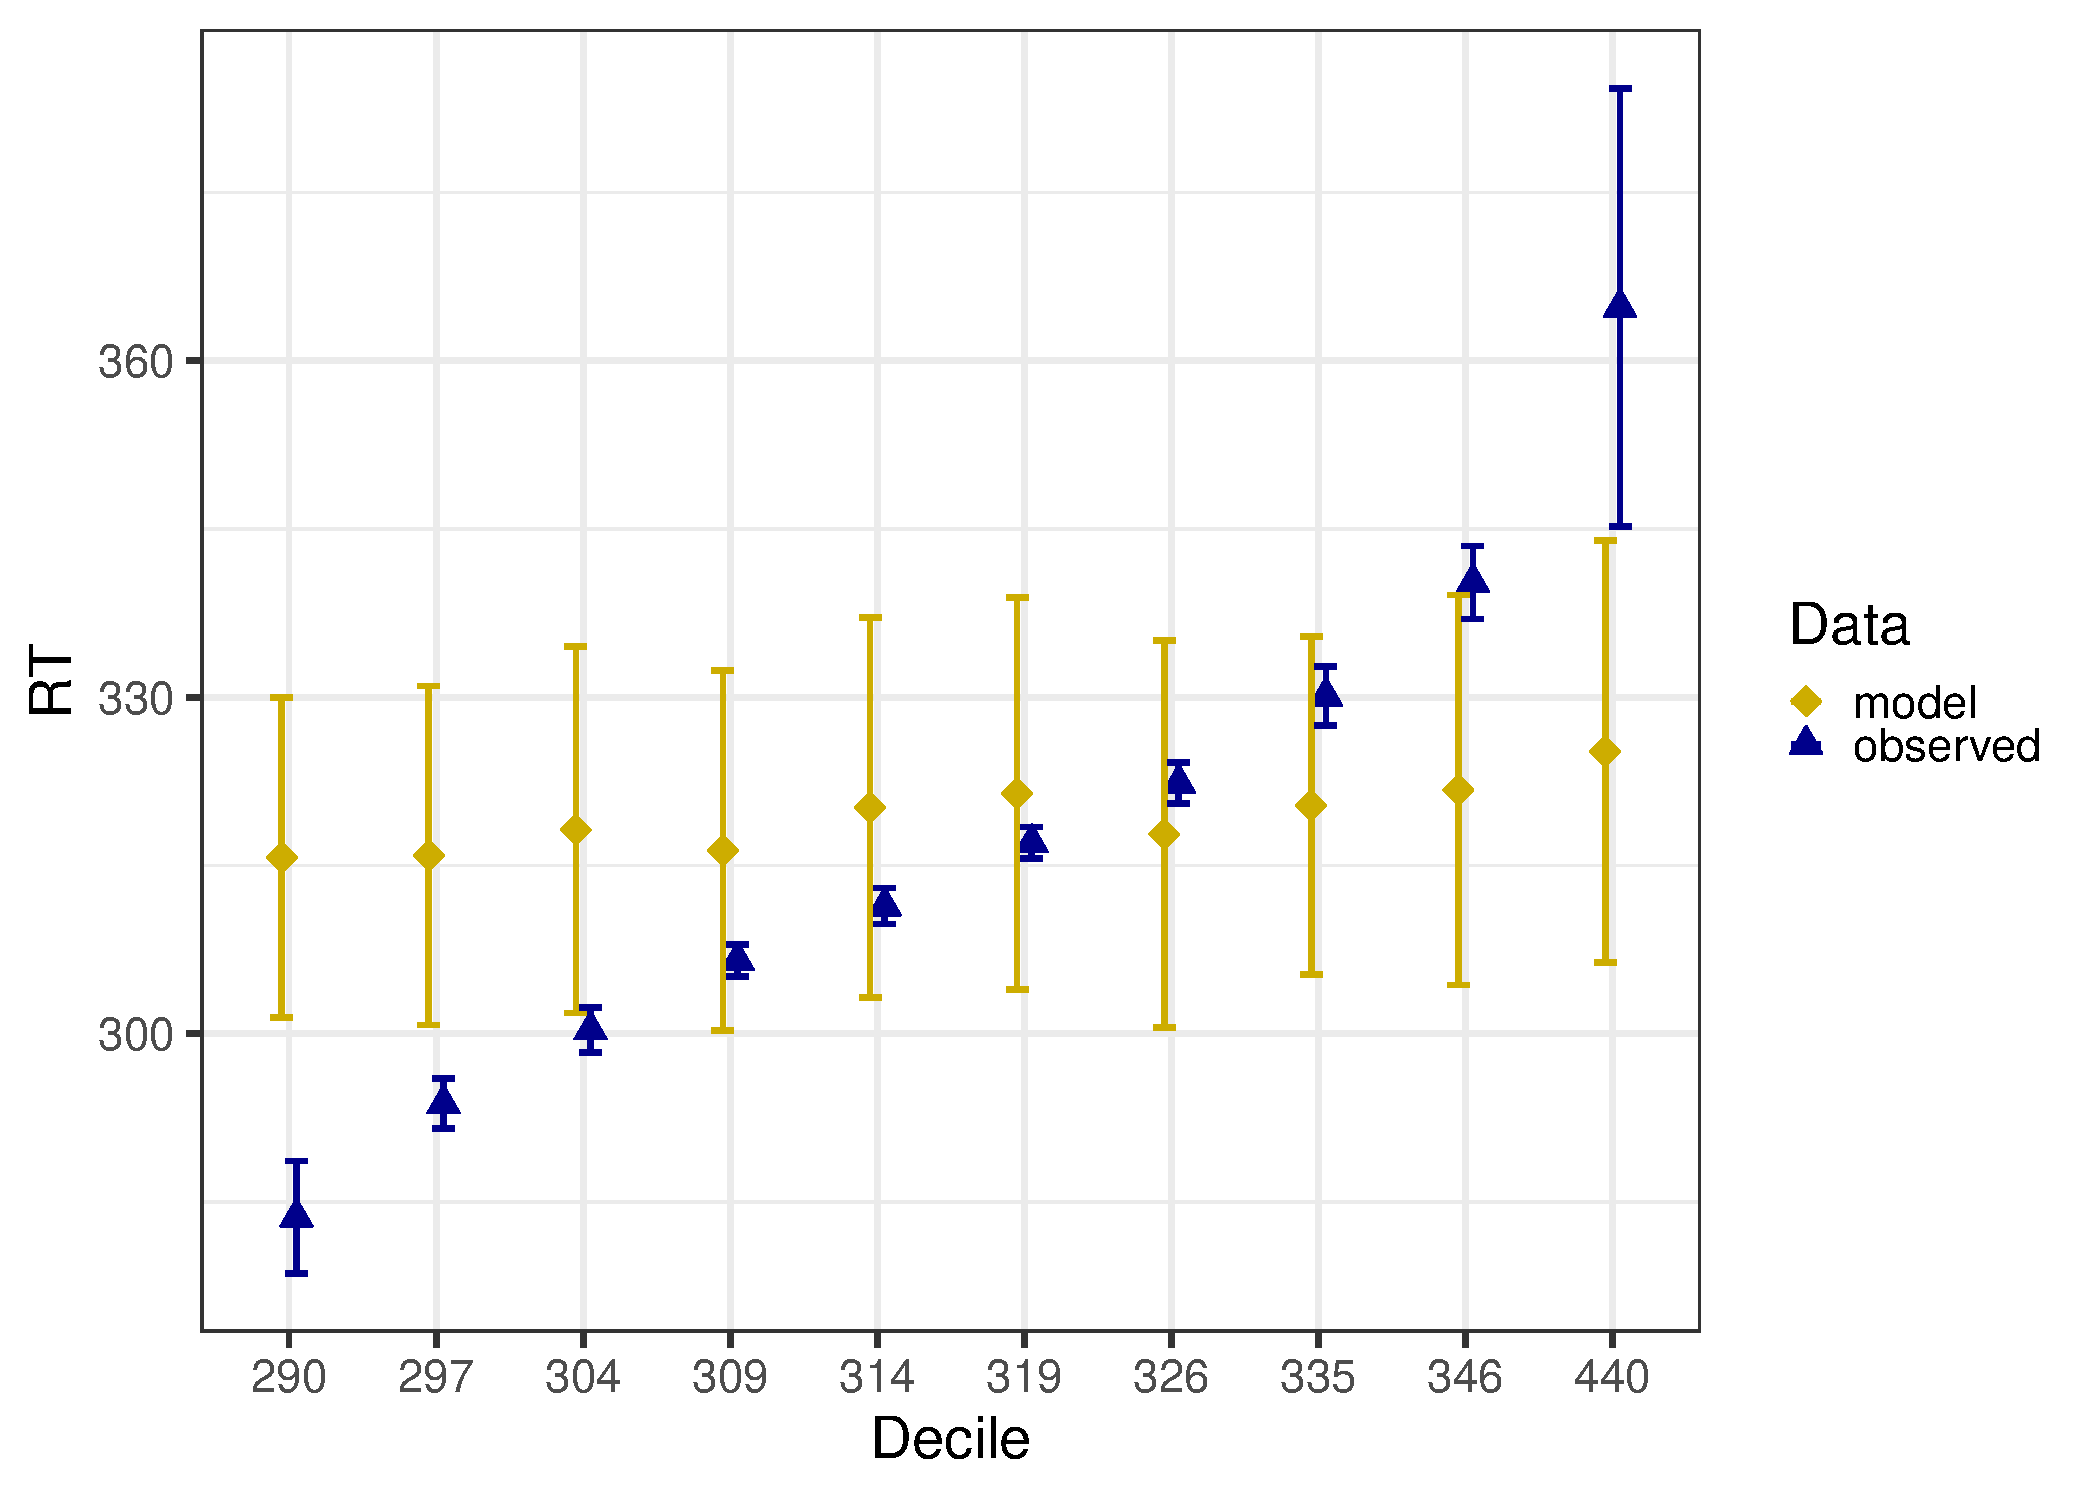
\includegraphics[width=\maxwidth]{figures/figure_ns_unnamed-chunk-19-1} 

\end{knitrout}

\begin{knitrout}
\definecolor{shadecolor}{rgb}{0.969, 0.969, 0.969}\color{fgcolor}\begin{kframe}
\begin{alltt}
\hlkwd{ggsave}\hlstd{(}\hlstr{"direct.png"}\hlstd{,} \hlkwc{width} \hlstd{=} \hlnum{19}\hlstd{,} \hlkwc{height} \hlstd{=} \hlnum{12}\hlstd{)}
\end{alltt}


{\ttfamily\noindent\itshape\color{messagecolor}{\#\# geom\_path: Each group consists of only one observation. Do you need to\\\#\# adjust the group aesthetic?}}\end{kframe}
\end{knitrout}

\begin{knitrout}
\definecolor{shadecolor}{rgb}{0.969, 0.969, 0.969}\color{fgcolor}\begin{kframe}
\begin{alltt}
\hlkwd{library}\hlstd{(ggplot2)}

\hlkwd{library}\hlstd{(dplyr)}

\hlstd{dodge} \hlkwb{<-} \hlkwd{position_dodge}\hlstd{(}\hlkwc{width} \hlstd{=} \hlnum{0.2}\hlstd{)}

\hlstd{data.to.plot} \hlkwb{<-} \hlstd{data.all} \hlopt \hlkwd{group_by}\hlstd{(Region)} \hlopt \hlkwd{summarise}\hlstd{(}\hlkwc{Region} \hlstd{=} \hlkwd{first}\hlstd{(Region),}
    \hlkwc{Word} \hlstd{=} \hlkwd{first}\hlstd{(Word),} \hlkwc{CF1} \hlstd{=} \hlkwd{quantile}\hlstd{(RT,} \hlkwc{probs} \hlstd{=} \hlkwd{c}\hlstd{(}\hlnum{0.05}\hlstd{,} \hlnum{0.95}\hlstd{))[}\hlnum{1}\hlstd{],} \hlkwc{CF2} \hlstd{=} \hlkwd{quantile}\hlstd{(RT,}
        \hlkwc{probs} \hlstd{=} \hlkwd{c}\hlstd{(}\hlnum{0.05}\hlstd{,} \hlnum{0.95}\hlstd{))[}\hlnum{2}\hlstd{],} \hlkwc{RT} \hlstd{=} \hlkwd{mean}\hlstd{(RT),} \hlkwc{Observed} \hlstd{=} \hlkwd{first}\hlstd{(Observed))}

\hlkwd{head}\hlstd{(}\hlkwd{as.data.frame}\hlstd{(data.to.plot),} \hlkwc{n} \hlstd{=} \hlnum{30}\hlstd{)}
\end{alltt}
\begin{verbatim}
##     Region     Word     CF1   CF2       RT Observed
## 1  No_0001     said 306.100 307.5 306.7965 313.4706
## 2  No_0002     that 338.300 339.0 338.6296 306.6118
## 3  No_0003  whoever 349.600 353.0 351.3075 338.4706
## 4  No_0004    could 306.300 307.9 307.0910 308.4535
## 5  No_0005     kill 315.665 318.8 317.1842 310.8372
## 6  No_0006      the 305.100 305.4 305.2129 297.8235
## 7  No_0007     boar 354.300 358.4 356.2165 303.6471
## 8  No_0008      and 338.200 338.6 338.3613 286.7294
## 9  No_0009    bring 312.000 314.8 313.3989 288.5294
## 10 No_0010       as 305.600 306.6 306.0363 331.6118
## 11 No_0011    proof 319.400 323.2 321.2384 340.7294
## 12 No_0012      its 339.400 341.0 340.1558 300.5529
## 13 No_0013     head 309.000 311.5 310.2748 300.0235
## 14 No_0014       to 338.200 338.7 338.3726 294.4471
## 15 No_0015      the 305.100 305.4 305.2122 320.7647
## 16 No_0016    manor 321.800 326.2 323.9535 316.9059
## 17 No_0017    house 341.300 343.6 342.4565 328.8810
## 18 No_0018    would 339.000 340.3 339.6278 317.3333
## 19 No_0019       be 305.500 306.4 305.8833 321.4286
## 20 No_0020 rewarded 358.100 363.6 360.7593 305.4941
## 21 No_0021     with 338.500 339.4 338.9029 314.0941
## 22 No_0022     land 311.100 313.8 312.4871 328.3214
## 23 No_0023      and 305.200 305.6 305.3602 335.9762
## 24 No_0024      was 305.400 306.1 305.7151 316.2706
## 25 No_0025      the 305.100 305.4 305.2122 309.5301
## 26 No_0026   people 306.700 308.4 307.5020 316.0723
## 27 No_0027       of 305.200 305.6 305.3409 328.9036
## 28 No_0028 bradford 318.400 322.0 320.1783 324.0000
## 29 No_0029      and 338.200 338.6 338.3613 331.0353
## 30 No_0030      the 305.100 305.4 305.2122 293.8214
\end{verbatim}
\begin{alltt}
\hlstd{g1} \hlkwb{<-} \hlkwd{ggplot}\hlstd{(data.to.plot,} \hlkwd{aes}\hlstd{(Region, RT))}
\hlstd{g1} \hlkwb{<-} \hlstd{g1} \hlopt{+} \hlkwd{geom_point}\hlstd{(}\hlkwc{position} \hlstd{= dodge,} \hlkwc{size} \hlstd{=} \hlkwd{I}\hlstd{(}\hlnum{5}\hlstd{))} \hlopt{+} \hlkwd{geom_errorbar}\hlstd{(}\hlkwd{aes}\hlstd{(}\hlkwc{ymin} \hlstd{= CF1,}
    \hlkwc{ymax} \hlstd{= CF2),} \hlkwc{position} \hlstd{= dodge,} \hlkwc{width} \hlstd{=} \hlnum{0.3}\hlstd{,} \hlkwc{size} \hlstd{=} \hlkwd{I}\hlstd{(}\hlnum{1.3}\hlstd{))} \hlopt{+} \hlkwd{scale_shape_manual}\hlstd{(}\hlkwc{values} \hlstd{=} \hlnum{21}\hlopt{:}\hlnum{24}\hlstd{)} \hlopt{+}
    \hlkwd{scale_color_manual}\hlstd{(}\hlkwc{values} \hlstd{=} \hlkwd{c}\hlstd{(}\hlstr{"gold3"}\hlstd{,} \hlstr{"blue4"}\hlstd{))} \hlopt{+} \hlkwd{scale_fill_manual}\hlstd{(}\hlkwc{values} \hlstd{=} \hlkwd{c}\hlstd{(}\hlstr{"gold3"}\hlstd{,}
    \hlstr{"blue4"}\hlstd{))} \hlopt{+} \hlkwd{theme_bw}\hlstd{(}\hlnum{28}\hlstd{)} \hlopt{+} \hlkwd{theme}\hlstd{(}\hlkwc{axis.text.x} \hlstd{=} \hlkwd{element_blank}\hlstd{())}
\hlstd{g1} \hlkwb{<-} \hlstd{g1} \hlopt{+} \hlkwd{geom_point}\hlstd{(}\hlkwd{aes}\hlstd{(}\hlkwc{x} \hlstd{= Region,} \hlkwc{y} \hlstd{= Observed),} \hlkwc{pch} \hlstd{=} \hlnum{24}\hlstd{,} \hlkwc{position} \hlstd{= dodge,}
    \hlkwc{size} \hlstd{=} \hlnum{4}\hlstd{)}
\end{alltt}
\end{kframe}
\end{knitrout}

\begin{knitrout}
\definecolor{shadecolor}{rgb}{0.969, 0.969, 0.969}\color{fgcolor}
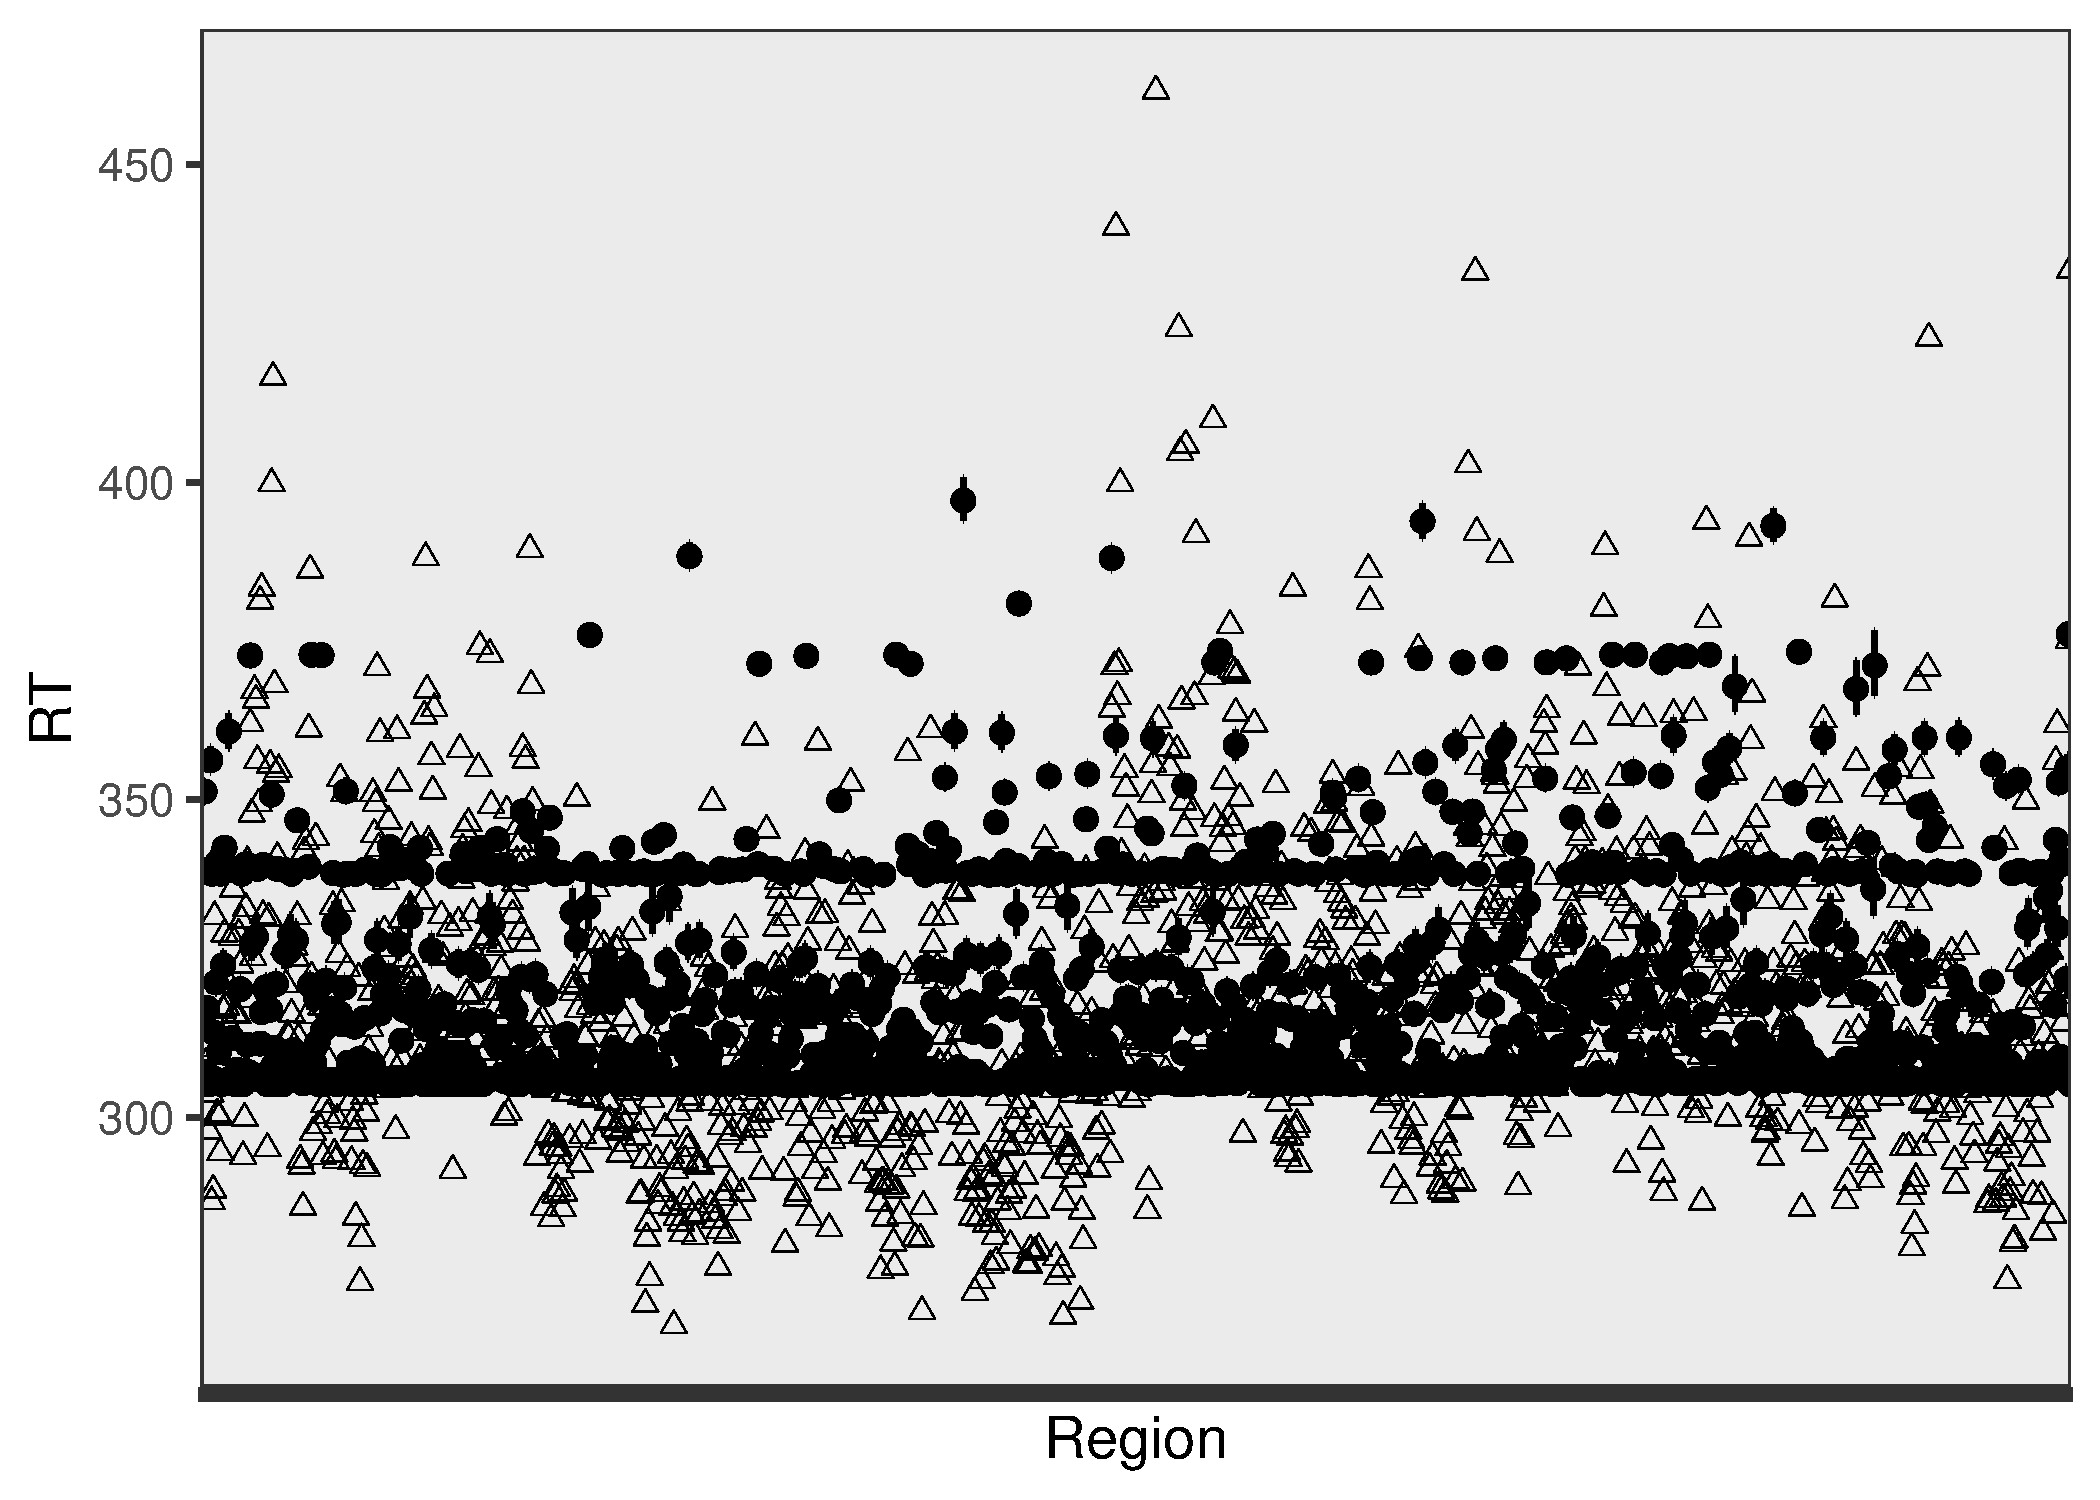
\includegraphics[width=\maxwidth]{figures/figure_ns_unnamed-chunk-22-1} 

\end{knitrout}

\begin{knitrout}
\definecolor{shadecolor}{rgb}{0.969, 0.969, 0.969}\color{fgcolor}\begin{kframe}
\begin{alltt}
\hlstd{g1} \hlkwb{<-} \hlkwd{ggplot}\hlstd{(data.to.plot,} \hlkwd{aes}\hlstd{(RT, Observed))}
\hlstd{g1} \hlkwb{<-} \hlstd{g1} \hlopt{+} \hlkwd{geom_point}\hlstd{(}\hlkwc{size} \hlstd{=} \hlkwd{I}\hlstd{(}\hlnum{2}\hlstd{),} \hlkwc{pch} \hlstd{=} \hlnum{24}\hlstd{)} \hlopt{+} \hlkwd{geom_errorbar}\hlstd{(}\hlkwd{aes}\hlstd{(}\hlkwc{ymin} \hlstd{= CF1,}
    \hlkwc{ymax} \hlstd{= CF2),} \hlkwc{position} \hlstd{= dodge,} \hlkwc{width} \hlstd{=} \hlnum{0.3}\hlstd{,} \hlkwc{size} \hlstd{=} \hlkwd{I}\hlstd{(}\hlnum{0.9}\hlstd{))} \hlopt{+} \hlkwd{scale_shape_manual}\hlstd{(}\hlkwc{values} \hlstd{=} \hlnum{21}\hlopt{:}\hlnum{24}\hlstd{)} \hlopt{+}
    \hlkwd{scale_color_manual}\hlstd{(}\hlkwc{values} \hlstd{=} \hlkwd{c}\hlstd{(}\hlstr{"gold3"}\hlstd{,} \hlstr{"blue4"}\hlstd{))} \hlopt{+} \hlkwd{scale_fill_manual}\hlstd{(}\hlkwc{values} \hlstd{=} \hlkwd{c}\hlstd{(}\hlstr{"gold3"}\hlstd{,}
    \hlstr{"blue4"}\hlstd{))} \hlopt{+} \hlkwd{theme_bw}\hlstd{(}\hlnum{28}\hlstd{)}
\hlstd{g1} \hlkwb{<-} \hlstd{g1} \hlopt{+} \hlkwd{geom_point}\hlstd{(}\hlkwd{aes}\hlstd{(}\hlkwc{x} \hlstd{= RT,} \hlkwc{y} \hlstd{= RT),} \hlkwc{pch} \hlstd{=} \hlnum{10}\hlstd{)}
\end{alltt}
\end{kframe}
\end{knitrout}

\begin{knitrout}
\definecolor{shadecolor}{rgb}{0.969, 0.969, 0.969}\color{fgcolor}\begin{kframe}


{\ttfamily\noindent\color{warningcolor}{\#\# Warning: position\_dodge requires non-overlapping x intervals}}\end{kframe}
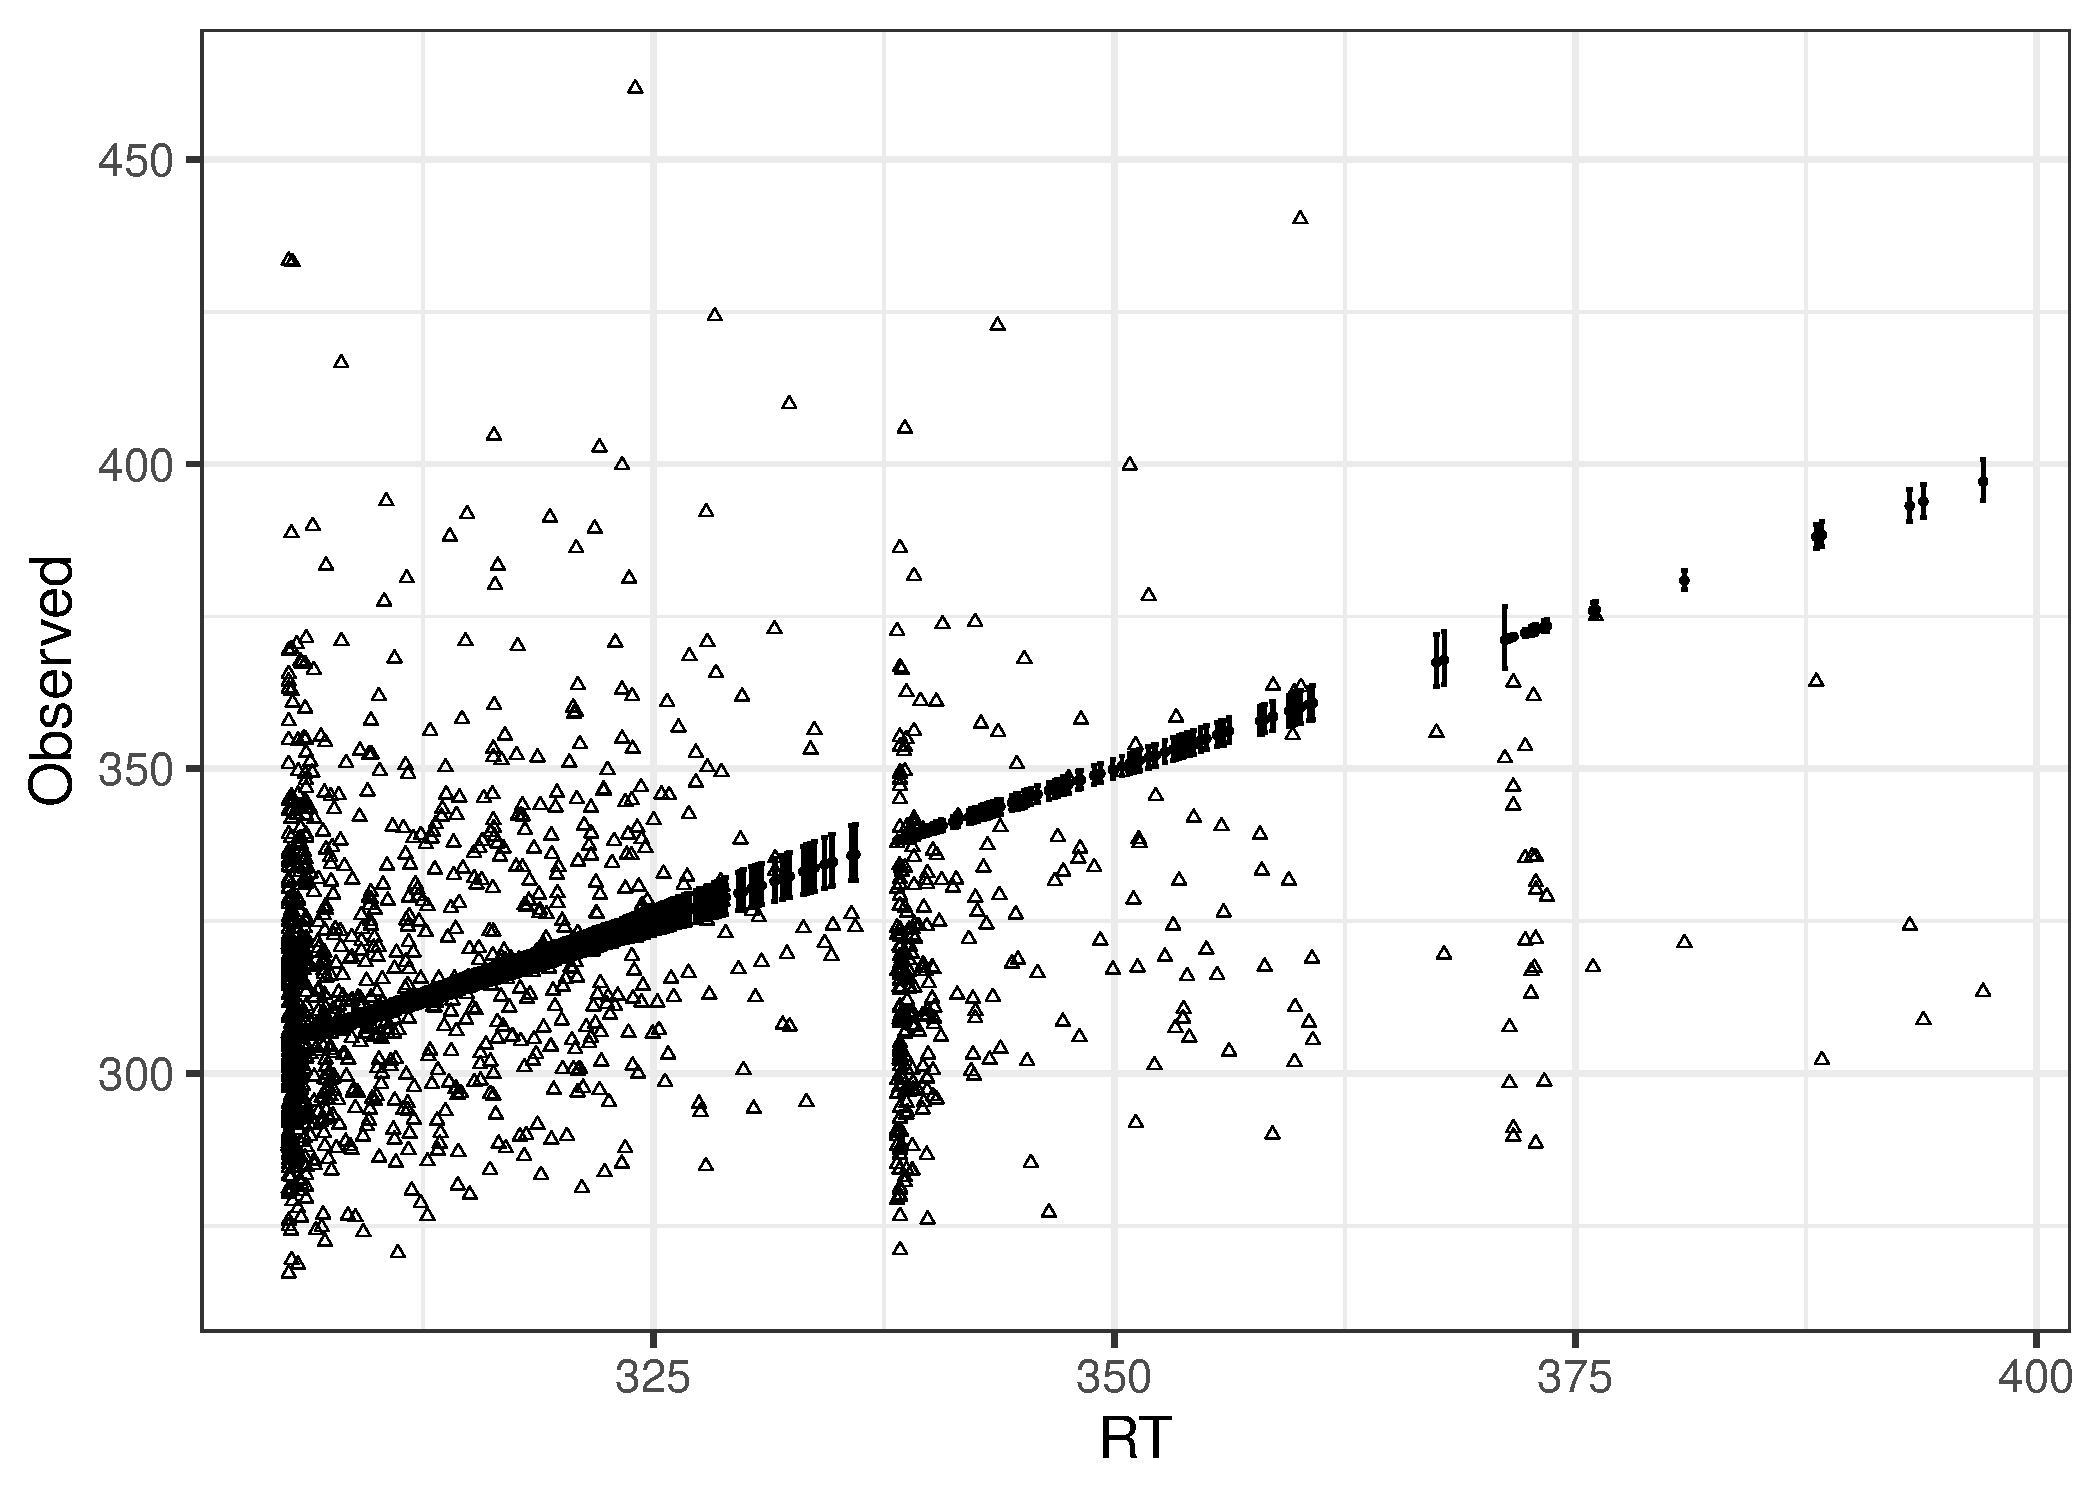
\includegraphics[width=\maxwidth]{figures/figure_ns_unnamed-chunk-24-1} 

\end{knitrout}


\begin{knitrout}
\definecolor{shadecolor}{rgb}{0.969, 0.969, 0.969}\color{fgcolor}\begin{kframe}
\begin{alltt}
\hlkwd{ggsave}\hlstd{(}\hlstr{"predictions-observed.png"}\hlstd{)}
\end{alltt}


{\ttfamily\noindent\itshape\color{messagecolor}{\#\# Saving 7 x 7 in image}}

{\ttfamily\noindent\color{warningcolor}{\#\# Warning: position\_dodge requires non-overlapping x intervals}}\end{kframe}
\end{knitrout}

\begin{knitrout}
\definecolor{shadecolor}{rgb}{0.969, 0.969, 0.969}\color{fgcolor}\begin{kframe}
\begin{alltt}
\hlstd{data.to.plot}\hlopt{$}\hlstd{RTadjusted} \hlkwb{<-} \hlstd{data.to.plot}\hlopt{$}\hlstd{RT} \hlopt{+} \hlstd{m2}\hlopt{$}\hlstd{coefficients[}\hlnum{3}\hlstd{]} \hlopt{*} \hlkwd{log}\hlstd{(}\hlkwd{as.numeric}\hlstd{(data.to.plot}\hlopt{$}\hlstd{Region))}
\hlstd{data.to.plot}\hlopt{$}\hlstd{Observedadjusted} \hlkwb{<-} \hlstd{data.to.plot}\hlopt{$}\hlstd{Observed} \hlopt{+} \hlstd{m2}\hlopt{$}\hlstd{coefficients[}\hlnum{3}\hlstd{]} \hlopt{*}
    \hlkwd{log}\hlstd{(}\hlkwd{as.numeric}\hlstd{(data.to.plot}\hlopt{$}\hlstd{Region))}
\hlstd{data.to.plot}\hlopt{$}\hlstd{CF1adjusted} \hlkwb{<-} \hlstd{data.to.plot}\hlopt{$}\hlstd{CF1} \hlopt{+} \hlstd{m2}\hlopt{$}\hlstd{coefficients[}\hlnum{3}\hlstd{]} \hlopt{*} \hlkwd{log}\hlstd{(}\hlkwd{as.numeric}\hlstd{(data.to.plot}\hlopt{$}\hlstd{Region))}
\hlstd{data.to.plot}\hlopt{$}\hlstd{CF2adjusted} \hlkwb{<-} \hlstd{data.to.plot}\hlopt{$}\hlstd{CF2} \hlopt{+} \hlstd{m2}\hlopt{$}\hlstd{coefficients[}\hlnum{3}\hlstd{]} \hlopt{*} \hlkwd{log}\hlstd{(}\hlkwd{as.numeric}\hlstd{(data.to.plot}\hlopt{$}\hlstd{Region))}

\hlstd{data.to.plot}
\end{alltt}
\begin{verbatim}
## # A tibble: 1,311 x 10
##    Region Word    CF1   CF2    RT Observed RTadjusted Observedadjusted
##    <fct>  <fct> <dbl> <dbl> <dbl>    <dbl>      <dbl>            <dbl>
##  1 No_00~ said   306.  308.  307.     313.       307.             313.
##  2 No_00~ that   338.  339.  339.     307.       350.             318.
##  3 No_00~ whoe~  350.  353   351.     338.       369.             356.
##  4 No_00~ could  306.  308.  307.     308.       329.             331.
##  5 No_00~ kill   316.  319.  317.     311.       343.             336.
##  6 No_00~ the    305.  305.  305.     298.       334.             326.
##  7 No_00~ boar   354.  358.  356.     304.       387.             335.
##  8 No_00~ and    338.  339.  338.     287.       371.             320.
##  9 No_00~ bring  312.  315.  313.     289.       348.             324.
## 10 No_00~ as     306.  307.  306.     332.       343.             368.
## # ... with 1,301 more rows, and 2 more variables: CF1adjusted <dbl>,
## #   CF2adjusted <dbl>
\end{verbatim}
\begin{alltt}
\hlstd{g1} \hlkwb{<-} \hlkwd{ggplot}\hlstd{(data.to.plot,} \hlkwd{aes}\hlstd{(RTadjusted, RTadjusted))}
\hlstd{g1} \hlkwb{<-} \hlstd{g1} \hlopt{+} \hlkwd{geom_point}\hlstd{(}\hlkwc{size} \hlstd{=} \hlkwd{I}\hlstd{(}\hlnum{2}\hlstd{))} \hlopt{+} \hlkwd{geom_errorbar}\hlstd{(}\hlkwd{aes}\hlstd{(}\hlkwc{ymin} \hlstd{= CF1adjusted,}
    \hlkwc{ymax} \hlstd{= CF2adjusted),} \hlkwc{width} \hlstd{=} \hlnum{0.3}\hlstd{,} \hlkwc{size} \hlstd{=} \hlkwd{I}\hlstd{(}\hlnum{0.9}\hlstd{))} \hlopt{+} \hlkwd{scale_shape_manual}\hlstd{(}\hlkwc{values} \hlstd{=} \hlnum{21}\hlopt{:}\hlnum{24}\hlstd{)} \hlopt{+}
    \hlkwd{scale_color_manual}\hlstd{(}\hlkwc{values} \hlstd{=} \hlkwd{c}\hlstd{(}\hlstr{"gold3"}\hlstd{,} \hlstr{"blue4"}\hlstd{))} \hlopt{+} \hlkwd{scale_fill_manual}\hlstd{(}\hlkwc{values} \hlstd{=} \hlkwd{c}\hlstd{(}\hlstr{"gold2"}\hlstd{,}
    \hlstr{"blue4"}\hlstd{))} \hlopt{+} \hlkwd{theme_bw}\hlstd{(}\hlnum{28}\hlstd{)}
\hlstd{g1} \hlkwb{<-} \hlstd{g1} \hlopt{+} \hlkwd{geom_point}\hlstd{(}\hlkwd{aes}\hlstd{(}\hlkwc{x} \hlstd{= RTadjusted,} \hlkwc{y} \hlstd{= Observedadjusted),} \hlkwc{pch} \hlstd{=} \hlnum{24}\hlstd{,}
    \hlkwc{size} \hlstd{=} \hlnum{4}\hlstd{)}
\end{alltt}
\end{kframe}
\end{knitrout}

\begin{knitrout}
\definecolor{shadecolor}{rgb}{0.969, 0.969, 0.969}\color{fgcolor}
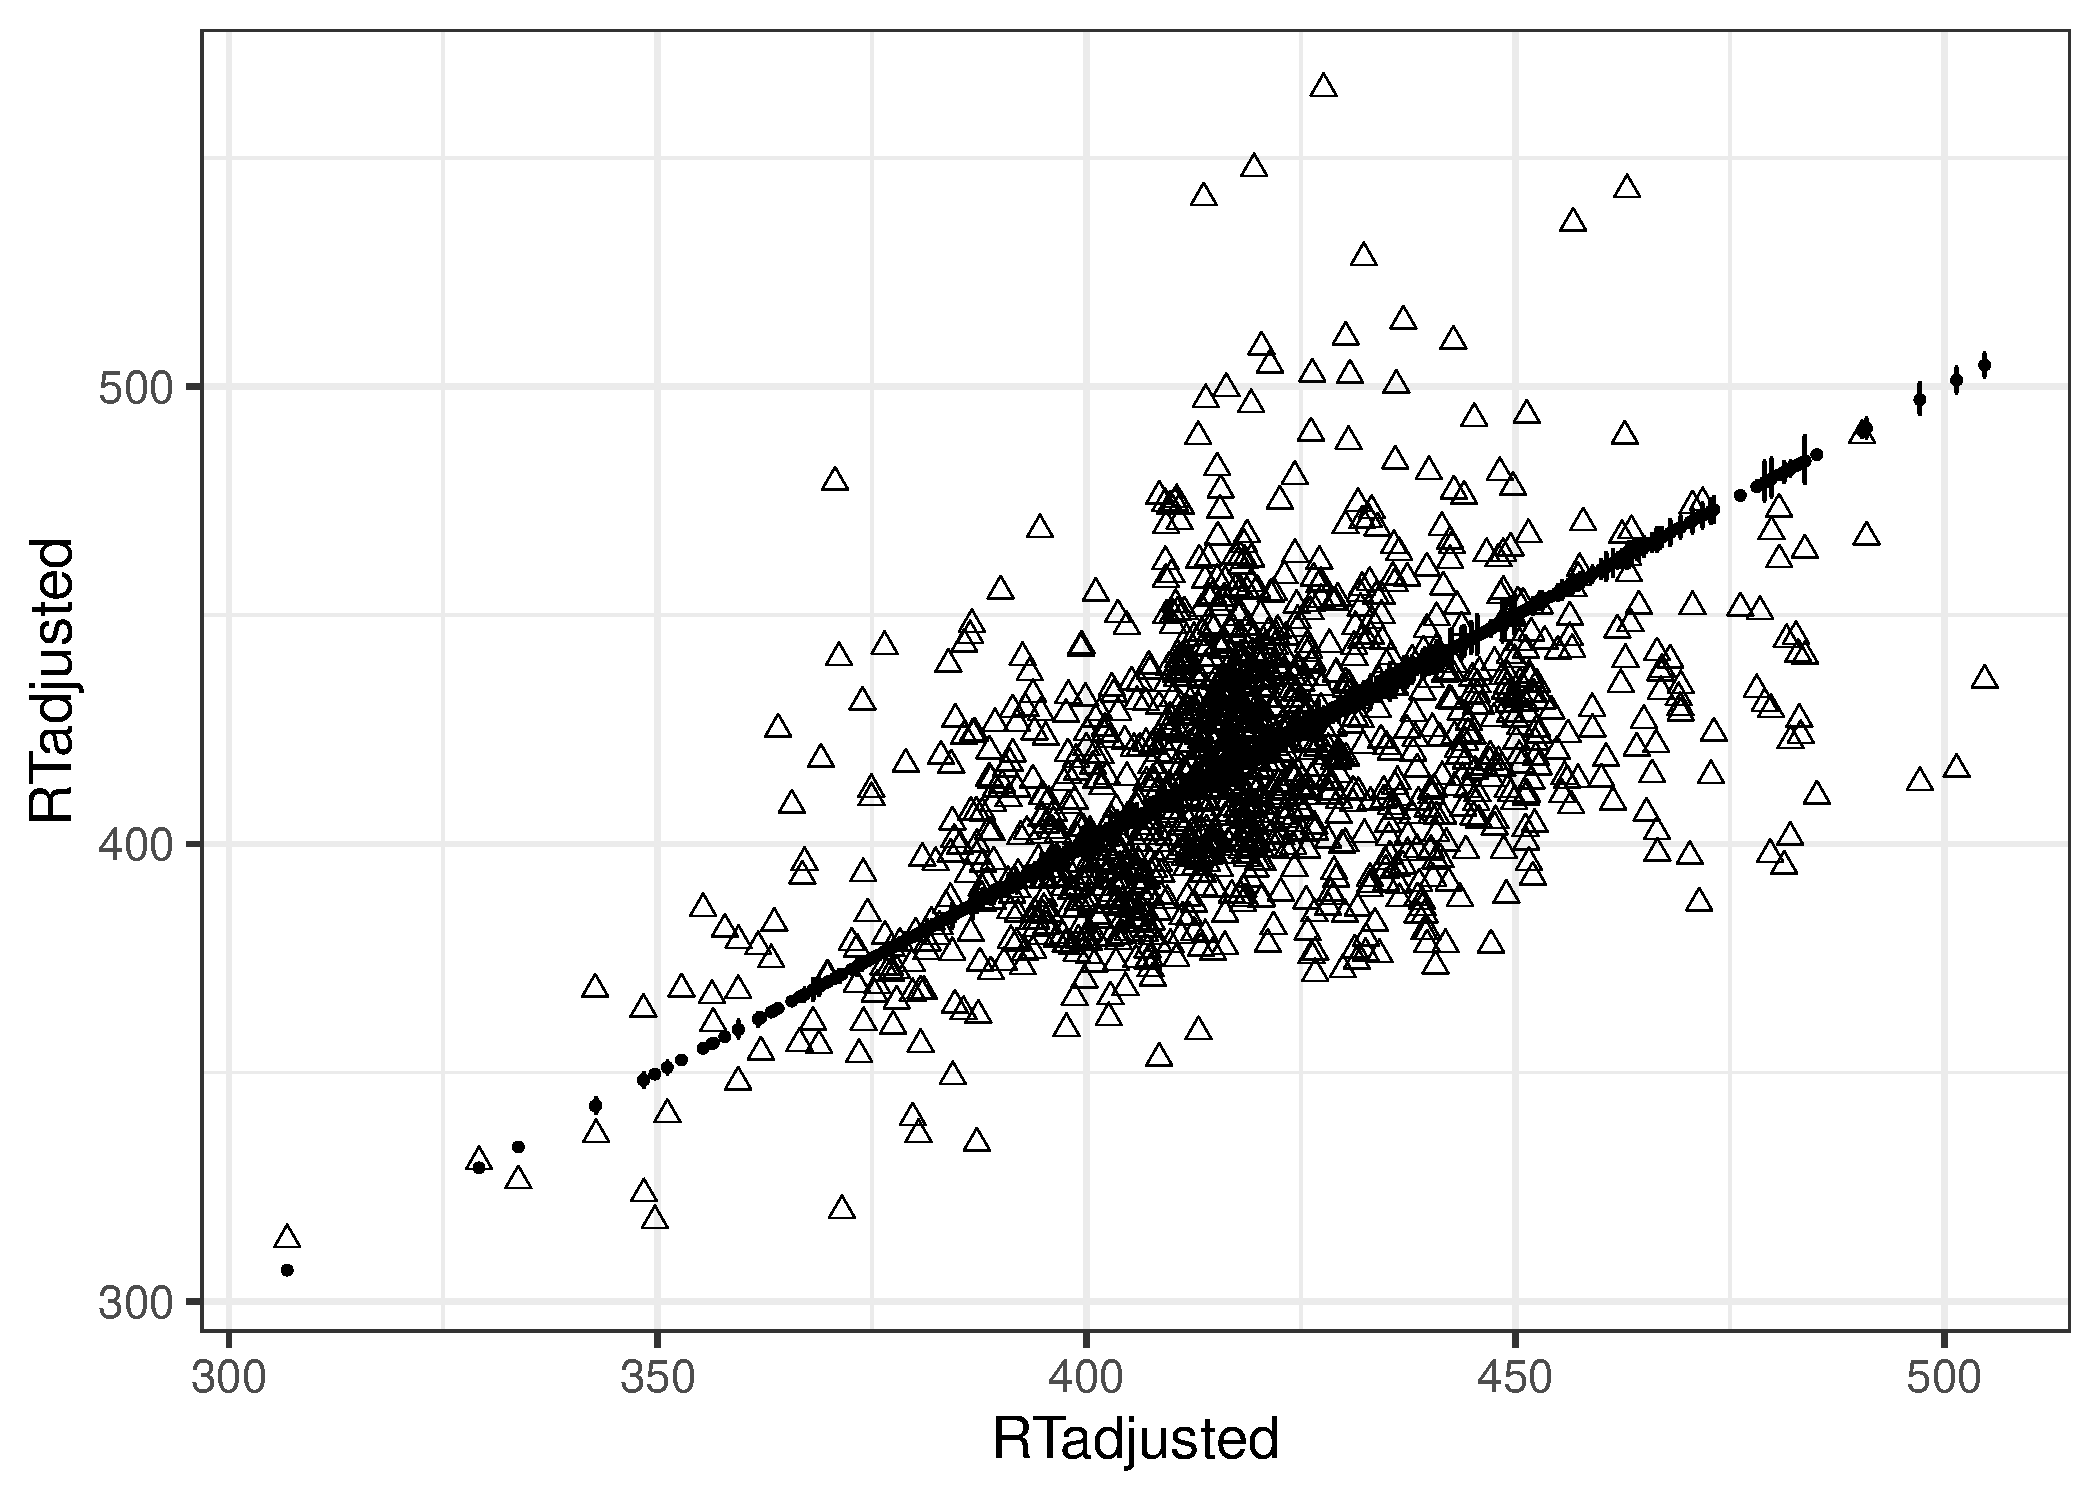
\includegraphics[width=\maxwidth]{figures/figure_ns_unnamed-chunk-27-1} 

\end{knitrout}

\begin{knitrout}
\definecolor{shadecolor}{rgb}{0.969, 0.969, 0.969}\color{fgcolor}\begin{kframe}
\begin{alltt}
\hlkwd{ggsave}\hlstd{(}\hlstr{"ns1.png"}\hlstd{)}
\end{alltt}


{\ttfamily\noindent\itshape\color{messagecolor}{\#\# Saving 7 x 7 in image}}\end{kframe}
\end{knitrout}


\section{Parameters}

This last part shows the values of parameters and Rhat values.



\subsection{LF}

\begin{knitrout}
\definecolor{shadecolor}{rgb}{0.969, 0.969, 0.969}\color{fgcolor}\begin{kframe}
\begin{alltt}
\hlcom{############# PARAMS###########}
\hlstd{draws} \hlkwb{<-} \hlkwd{createdraws}\hlstd{(}\hlstr{"lf"}\hlstd{)}

\hlkwd{str}\hlstd{(draws)}
\end{alltt}
\begin{verbatim}
##  num [1:807, 1:2] 0.0126 0.0126 0.0126 0.016 0.016 ...
\end{verbatim}
\begin{alltt}
\hlkwd{Rhat}\hlstd{(draws)}
\end{alltt}
\begin{verbatim}
## [1] 1.036216
\end{verbatim}
\end{kframe}
\end{knitrout}

Mean etc.

\begin{knitrout}
\definecolor{shadecolor}{rgb}{0.969, 0.969, 0.969}\color{fgcolor}\begin{kframe}
\begin{alltt}
\hlkwd{tail}\hlstd{(draws)}
\end{alltt}
\begin{verbatim}
##              [,1]       [,2]
## [802,] 0.01420765 0.01337264
## [803,] 0.01420765 0.01337264
## [804,] 0.01420765 0.01337264
## [805,] 0.01420765 0.01337264
## [806,] 0.01420765 0.01337264
## [807,] 0.01420765 0.01337264
\end{verbatim}
\begin{alltt}
\hlkwd{mean}\hlstd{(}\hlkwd{c}\hlstd{(draws[,} \hlnum{1}\hlopt{:}\hlnum{2}\hlstd{]))}
\end{alltt}
\begin{verbatim}
## [1] 0.01390178
\end{verbatim}
\begin{alltt}
\hlkwd{median}\hlstd{(}\hlkwd{c}\hlstd{(draws[,} \hlnum{1}\hlopt{:}\hlnum{2}\hlstd{]))}
\end{alltt}
\begin{verbatim}
## [1] 0.01394016
\end{verbatim}
\begin{alltt}
\hlkwd{sd}\hlstd{(}\hlkwd{c}\hlstd{(draws[,} \hlnum{1}\hlopt{:}\hlnum{2}\hlstd{]))}
\end{alltt}
\begin{verbatim}
## [1] 0.001022104
\end{verbatim}
\end{kframe}
\end{knitrout}

\subsection{LE}

\begin{knitrout}
\definecolor{shadecolor}{rgb}{0.969, 0.969, 0.969}\color{fgcolor}\begin{kframe}
\begin{alltt}
\hlcom{############# PARAMS###########}
\hlstd{draws} \hlkwb{<-} \hlkwd{createdraws}\hlstd{(}\hlstr{"le"}\hlstd{)}

\hlkwd{str}\hlstd{(draws)}
\end{alltt}
\begin{verbatim}
##  num [1:807, 1:2] 0.653 0.653 0.647 0.647 0.647 ...
\end{verbatim}
\begin{alltt}
\hlkwd{Rhat}\hlstd{(draws)}
\end{alltt}
\begin{verbatim}
## [1] 1.027879
\end{verbatim}
\end{kframe}
\end{knitrout}

Mean etc.

\begin{knitrout}
\definecolor{shadecolor}{rgb}{0.969, 0.969, 0.969}\color{fgcolor}\begin{kframe}
\begin{alltt}
\hlkwd{tail}\hlstd{(draws)}
\end{alltt}
\begin{verbatim}
##             [,1]      [,2]
## [802,] 0.6308769 0.6710766
## [803,] 0.6308769 0.6710766
## [804,] 0.6308769 0.6710766
## [805,] 0.6308769 0.6710766
## [806,] 0.6308769 0.6710766
## [807,] 0.6308769 0.6710766
\end{verbatim}
\begin{alltt}
\hlkwd{mean}\hlstd{(}\hlkwd{c}\hlstd{(draws[,} \hlnum{1}\hlopt{:}\hlnum{2}\hlstd{]))}
\end{alltt}
\begin{verbatim}
## [1] 0.6611395
\end{verbatim}
\begin{alltt}
\hlkwd{median}\hlstd{(}\hlkwd{c}\hlstd{(draws[,} \hlnum{1}\hlopt{:}\hlnum{2}\hlstd{]))}
\end{alltt}
\begin{verbatim}
## [1] 0.654711
\end{verbatim}
\begin{alltt}
\hlkwd{sd}\hlstd{(}\hlkwd{c}\hlstd{(draws[,} \hlnum{1}\hlopt{:}\hlnum{2}\hlstd{]))}
\end{alltt}
\begin{verbatim}
## [1] 0.0681144
\end{verbatim}
\end{kframe}
\end{knitrout}

\end{document}
